\documentclass[12pt,a4paper]{report}

%% ============================================================
%% PACKAGES
%% ============================================================
\usepackage[a4paper,top=30mm,bottom=25mm,left=30mm,right=30mm,headheight=15pt]{geometry}
\usepackage{fancyhdr}
\setlength{\headheight}{15pt}
\usepackage{amsmath,amssymb}
\usepackage{booktabs}
\usepackage{colortbl}
\usepackage{longtable}
\usepackage{array}
\usepackage{multirow}
\usepackage{xcolor}
\usepackage{tikz}
\usepackage{pgfplots}
\pgfplotsset{compat=1.18}
\usetikzlibrary{shapes.geometric,arrows.meta,positioning,calc,backgrounds,
                patterns,decorations.pathreplacing}
\usepackage[framemethod=tikz]{mdframed}
\usepackage{titlesec}
\usepackage{tocloft}
\usepackage{setspace}
\usepackage{caption}
\usepackage{subcaption}
\usepackage{enumitem}
\usepackage{hyperref}
\usepackage{cite}
\usepackage{float}
\usepackage{tabularx}
\usepackage[T1]{fontenc}
\usepackage{parskip}
\usepackage{pgfgantt}
\usepackage{eso-pic}
\usepackage{makecell}
\usepackage{ragged2e}
\usepackage{pdflscape}
\usepackage{lastpage}
\usepackage{siunitx}
\usepackage{graphicx}
\graphicspath{{figures/}{./}}
\usepackage{rotating}

\usepackage{pdfpages}
\sisetup{separate-uncertainty=true}

%% ============================================================
%% COLOURS
%% ============================================================
\definecolor{uqpurple}{RGB}{81,36,122}
\definecolor{uqgold}{RGB}{187,155,28}
\definecolor{accentblue}{RGB}{0,100,180}
\definecolor{tableheader}{RGB}{220,210,235}
\definecolor{rowgray}{RGB}{248,248,252}
\definecolor{resultgreen}{RGB}{0,120,60}
\definecolor{warnorange}{RGB}{180,80,0}
\definecolor{deepred}{RGB}{160,0,0}

%% ============================================================
%% PAGE BORDER
%% ============================================================
\newcommand\PageBorder{%
\begin{tikzpicture}[remember picture,overlay]
\draw[line width=1.8pt,color=uqpurple]
  ([xshift=13mm,yshift=-13mm]current page.north west)
  rectangle ([xshift=-13mm,yshift=13mm]current page.south east);
\end{tikzpicture}}
\AddToShipoutPictureBG{\PageBorder}

%% ============================================================
%% HEADER / FOOTER
%% ============================================================
\pagestyle{fancy}
\fancyhf{}
\fancyhead[L]{\small\color{uqpurple}\textit{Engineering Thesis: Final Report}}
\fancyhead[R]{\small\color{uqpurple}\textit{Performance of CO$_2$ Cycle --- Energy Transition}}
\fancyfoot[L]{\small\color{uqpurple}Vennkkata Reddi Cheemalapati \textbar\ 46555991}
\fancyfoot[C]{\small\color{uqpurple}Page \thepage\ of \pageref{LastPage}}
\fancyfoot[R]{\small\color{uqpurple}ENGG4600 \textbar\ UQ \textbar\ 2026}
\renewcommand{\headrulewidth}{0.8pt}
\renewcommand{\headrule}{\hbox to\headwidth{%
  \color{uqpurple}\leaders\hrule height\headrulewidth\hfill}}
\renewcommand{\footrulewidth}{0.6pt}
\renewcommand{\footrule}{\hbox to\headwidth{%
  \color{uqgold}\leaders\hrule height\footrulewidth\hfill}}
\fancypagestyle{plain}{%
  \fancyhf{}
  \fancyfoot[L]{\small\color{uqpurple}Vennkkata Reddi Cheemalapati}
  \fancyfoot[C]{\small\color{uqpurple}Page \thepage\ of \pageref{LastPage}}
  \fancyfoot[R]{\small\color{uqpurple}ENGG4600 \textbar\ UQ \textbar\ 2026}
  \renewcommand{\headrulewidth}{0pt}
  \renewcommand{\footrulewidth}{0.6pt}
  \renewcommand{\footrule}{\hbox to\headwidth{%
    \color{uqgold}\leaders\hrule height\footrulewidth\hfill}}
}

%% ============================================================
%% SECTION FORMATTING
%% ============================================================
\titleformat{\chapter}[block]
  {\normalfont\Large\bfseries\color{uqpurple}}{\thechapter.}{0.8em}{}
  [\vspace{-0.4em}\color{uqpurple}\rule{\linewidth}{0.8pt}]
\titlespacing*{\chapter}{0pt}{-20pt}{12pt}
\titleformat{\section}[block]
  {\normalfont\large\bfseries\color{uqpurple}}{\thesection}{0.8em}{}
\titleformat{\subsection}[block]
  {\normalfont\normalsize\bfseries\color{accentblue}}{\thesubsection}{0.8em}{}
\titleformat{\subsubsection}[block]
  {\normalfont\normalsize\itshape\color{accentblue}}{\thesubsubsection}{0.8em}{}

\hypersetup{
  colorlinks=true,linkcolor=uqpurple,citecolor=accentblue,urlcolor=accentblue,
  pdftitle={Final Thesis: Performance of CO2 Cycle in the Context of Energy Transition},
  pdfauthor={Vennkkata Reddi Cheemalapati, UQ}
}

\captionsetup{font=small,labelfont={bf,color=uqpurple},margin=8pt,width=\linewidth}
\setstretch{1.25}
\setlength{\LTcapwidth}{\textwidth}

%% ============================================================
%% CUSTOM ENVIRONMENTS
%% ============================================================
\newmdenv[linecolor=resultgreen,linewidth=1.5pt,backgroundcolor=resultgreen!5,
  roundcorner=4pt,innerleftmargin=12pt,innerrightmargin=12pt,
  innertopmargin=8pt,innerbottommargin=8pt]{findingbox}

\newmdenv[linecolor=uqpurple,linewidth=1.5pt,backgroundcolor=uqpurple!5,
  roundcorner=4pt,innerleftmargin=12pt,innerrightmargin=12pt,
  innertopmargin=8pt,innerbottommargin=8pt]{insightbox}

\newmdenv[linecolor=warnorange,linewidth=1.5pt,backgroundcolor=warnorange!5,
  roundcorner=4pt,innerleftmargin=12pt,innerrightmargin=12pt,
  innertopmargin=8pt,innerbottommargin=8pt]{limitbox}

\newcommand{\keyresult}[1]{\textbf{\color{resultgreen}#1}}
\newcommand{\keyfinding}[1]{\textbf{\color{uqpurple}#1}}

%% Figure helper: PNG if present, otherwise a labelled placeholder
\newcommand{\pinchdummy}[2]{%
  \begin{tikzpicture}
    \fill[gray!10,rounded corners=4pt](0,0) rectangle (\linewidth,#1);
    \node[anchor=center,text=gray!55,font=\small\itshape]
      at (0.5\linewidth,#1/2)
      {Figure placeholder --- place \texttt{#2} alongside this .tex file};
  \end{tikzpicture}}

%% ============================================================

\newcommand{\thesisfig}[3]{%
  \IfFileExists{figures/#1}{\includegraphics[width=#2\textwidth]{#1}}{%
  \IfFileExists{#1}{\includegraphics[width=#2\textwidth]{#1}}{\pinchdummy{#3}{#1}}}}
\begin{document}
\let\cleardoublepage\clearpage
\hbadness=99999
\hfuzz=30pt
%% ============================================================
%% TITLE PAGE
%% ============================================================
\begin{titlepage}
\begin{tikzpicture}[remember picture,overlay]
  \fill[uqpurple](current page.north west)
    rectangle ([yshift=-5.2cm]current page.north east);
  \fill[uqgold]([yshift=-5.2cm]current page.north west)
    rectangle ([yshift=-5.75cm]current page.north east);
  \fill[uqpurple!15](current page.south west)
    rectangle ([yshift=2.4cm]current page.south east);
  \draw[white,line width=1pt,opacity=0.10,dashed]
    ([xshift=-2.5cm,yshift=-4.5cm]current page.north east) circle (6cm);
  \draw[white,line width=0.6pt,opacity=0.07,dashed]
    ([xshift=-1cm,yshift=-2cm]current page.north east) circle (3.5cm);
\end{tikzpicture}
\vspace*{2.9cm}
{\centering
  {\color{white}\Large\bfseries SCHOOL OF MECHANICAL AND MINING ENGINEERING}\\[0.25cm]
  {\color{white}\normalsize The University of Queensland}\\[0.15cm]
  {\color{uqgold}\small\bfseries Brisbane, Australia}\\[2.0cm]
  {\color{uqpurple}\LARGE\bfseries Engineering Thesis: Final Report}\\[0.3cm]
  {\color{uqpurple}\small\bfseries ENGG4600 --- 2026}\\[0.9cm]
  \begin{mdframed}[linecolor=uqpurple,linewidth=2pt,backgroundcolor=white,
    innerleftmargin=16pt,innerrightmargin=16pt,
    innertopmargin=16pt,innerbottommargin=16pt,roundcorner=4pt]
  {\centering\Large\bfseries\color{uqpurple}
    Performance of CO$_2$ Cycle in the\\[0.4em]
    Context of Energy Transition\par}
  \end{mdframed}
  \vspace{1.8cm}
  \begin{tabular}{p{4.5cm} p{9.0cm}}
    \textbf{Name:}         & Vennkkata Reddi Cheemalapati \\[0.4cm]
    \textbf{Student No.:}  & 46555991 \\[0.4cm]
    \textbf{Course Code:}  & ENGG4600 \\[0.4cm]
    \textbf{Supervisor:}   & Dr Alexander Klimenko \\[0.4cm]
    \textbf{Date:}         & 22 October 2026 \\[0.4cm]
    \textbf{Word Count:}   & $\approx$ 16,000 words (Chapters 1--9) \\[0.4cm]
    \textbf{Thesis Title:} &
      \parbox[t]{9.0cm}{\raggedright\itshape
        Performance of CO$_2$ Cycle in the Context of Energy Transition}\\
  \end{tabular}
\par}
\end{titlepage}
%% ============================================================
%% FRONT MATTER
%% ============================================================
\pagestyle{plain}
\pagenumbering{roman}

%% ============================================================
%% ABSTRACT
%% ============================================================
\chapter*{Abstract}
\addcontentsline{toc}{chapter}{Abstract}

This thesis compares three power cycles for industrial waste heat recovery
(WHR) in an Australian context --- the Steam Rankine Cycle (SRC), the
Supercritical CO$_2$ (sCO$_2$) Brayton cycle and the Transcritical CO$_2$
(tCO$_2$) Rankine cycle --- under one consistent set of thermodynamic,
sizing, cost and economic assumptions, applied to three representative
sites: LNG gas processing in the Pilbara (200\,\textdegree C, 30\,kg/s),
cement preheater exhaust in Gladstone (350\,\textdegree C, 50\,kg/s) and
electric arc furnace off-gas in Sydney (500\,\textdegree C, 20\,kg/s). Four
research questions address thermodynamic performance (RQ1), equipment sizing
and capital cost (RQ2), techno-economic viability (RQ3) and off-design
flexibility (RQ4). All models are implemented in Python with CoolProp and
every result is regenerated by a single script.

Thirty findings are reported. With the recuperator energy balance limited by
both streams --- a second-law requirement that the interim analysis did not
satisfy --- the steam cycle has the highest thermal efficiency at every
turbine inlet temperature from 150 to 600\,\textdegree C (19.1--35.4\,\%
against 13.3--30.1\,\% for tCO$_2$ and 5.3--30.1\,\% for sCO$_2$), and no
crossover occurs within the WHR range. A 200-node integration of the tCO$_2$
heater against a waste-gas stream whose temperature is linear in heat duty
shows a double pinch at both terminals with the driving force widest in the
middle (42--65\,K), so that two-point LMTD sizing overestimates heater area
by 129--223\,\% when the pseudo-critical $c_p$ peak lies inside the heater.
The CO$_2$ cycles' decisive weakness in Australia is the heat sink: the
tCO$_2$ baseline condenses at 14.3\,\textdegree C, which a chiller could
supply only by consuming 63--134\,\% of the net output, and the sCO$_2$ cycle
loses 42\,\% of its 200\,\textdegree C efficiency if its compressor inlet
warms from 32 to 40\,\textdegree C.

Integrated with each site's stream through a 10\,K-approach heater, the
steam boiler must run at 0.16--3.7\,MPa rather than 10\,MPa, and the tCO$_2$
cycle recovers the most power at 200 and 350\,\textdegree C (723 and
3418\,kW against 412 and 2639\,kW for steam) because its cold heater inlet
cools the gas furthest; the recuperated sCO$_2$ cycle recovers the least at
every site. CO$_2$ turbines are 15--26 times more compact than the steam
turbine, but at equal output steam is the cheapest plant at every site
(AUD\,2{,}600--4{,}400/kW at 1\,MWe in 2026), tCO$_2$ costs 30--65\,\% more
and sCO$_2$ two to three times more. On a fixed-source basis steam gives the
lowest LCOE at all three sites (AUD\,96, 35 and 31/MWh) and the highest NPV
with 3--4-year discounted paybacks and 99.8--100\,\% Monte Carlo viability at
350 and 500\,\textdegree C; tCO$_2$ is the better investment at
200\,\textdegree C (NPV AUD\,1.71\,M against 1.12\,M) only where a natural
cold sink exists; sCO$_2$ is not viable at any site. The tCO$_2$ cycle is
the most flexible at part load (Marchionni score 0.78 against 0.73 for steam
and 0.71 for sCO$_2$).

The thesis concludes that the figure of merit for WHR cycle selection is the
net work recovered per kilogram of waste gas and its cost, not thermal
efficiency, and that at Australian sink temperatures the steam Rankine cycle
is the default choice above 300\,\textdegree C, with transcritical CO$_2$
reserved for low-temperature sources where cold water is available.

\bigskip\noindent\textbf{Keywords:} CO$_2$ power cycle; waste heat recovery;
supercritical CO$_2$; transcritical CO$_2$; steam Rankine cycle; exergy
analysis; pseudo-critical; pinch analysis; techno-economic analysis; LCOE;
Australia; energy transition.

\clearpage

%% ============================================================
%% EXECUTIVE SUMMARY
%% ============================================================
\chapter*{Executive Summary}
\addcontentsline{toc}{chapter}{Executive Summary}

This report evaluates the commercial viability of retrofitting waste heat
recovery (WHR) power cycles at three Australian industrial sites: a Pilbara
LNG train (200\,\textdegree C), a Gladstone cement preheater
(350\,\textdegree C) and a Sydney electric arc furnace (500\,\textdegree C).
Three cycles --- Steam Rankine (SRC), Supercritical CO$_2$ Brayton (sCO$_2$)
and Transcritical CO$_2$ Rankine (tCO$_2$) --- were modelled on one
consistent basis, each sized to what it can recover from the site's exhaust
stream and costed at that size in 2026 Australian dollars.

\textbf{Key findings for capital allocation:}
\begin{itemize}[leftmargin=1.5em,itemsep=6pt]
\item \textbf{High- and medium-temperature WHR (350--500\,\textdegree C):}
The steam Rankine cycle is the clear choice. It is the most efficient of the
three under Australian sink conditions, the cheapest to build
(AUD\,1{,}900--2{,}200/kW at the 2.3--2.6\,MWe site scale), and the most
bankable: LCOE of AUD\,31--35/MWh against site prices of 90--100/MWh,
discounted payback of 3.2--4.2 years, IRR of 28--36\,\%, and positive NPV in
99.8--100\,\% of 10,000 cost, price and utilisation scenarios.
\item \textbf{Low-temperature WHR (200\,\textdegree C):} Marginal for any
cycle. Steam and tCO$_2$ both return about 12\,\% IRR with a one-in-three
chance of loss, and depend on the Pilbara price premium. The tCO$_2$ cycle
recovers 75\,\% more electricity from the stream and has 53\,\% more NPV, but
only if a heat sink near 4\,\textdegree C is available; supplying it with a
chiller would consume more power than the plant makes.
\item \textbf{Supercritical CO$_2$:} Not investable in its simple recuperated
form at any of the three sites. With cooling water that cannot bring the
compressor inlet below 36\,\textdegree C, the cycle's back-work ratio is
31--64\,\%, its turbomachinery costs more than a whole steam plant, and its
recuperated heater leaves most of the exhaust heat unrecovered. NPV is
negative at two sites and marginal at the third.
\item \textbf{Flexibility:} Where the heat source fluctuates (batch
furnaces, intermittent trains), the tCO$_2$ cycle retains 56--67\,\% of its
efficiency at one-fifth load against 38--66\,\% for steam, and starts up most
simply.
\end{itemize}

\textbf{Investment recommendation:}\\
Target \textbf{steam Rankine} technology for Australian WHR sources at
350\,\textdegree C and above. Treat 200\,\textdegree C sources as
site-specific studies, with transcritical CO$_2$ preferred only where cold
water or a co-located refrigeration load exists. Do not pursue simple
supercritical CO$_2$ Brayton systems below 500\,\textdegree C in Australian
conditions. Evaluate every option on the electricity recovered from the
actual stream and its cost, not on thermal efficiency.

\clearpage

%% ============================================================
%% DECLARATION
%% ============================================================
\chapter*{Declaration by Author}
\addcontentsline{toc}{chapter}{Declaration by Author}
%% STUDENT: read every sentence of this declaration and edit it so that it
%% describes exactly what you did and what the AI tools did. Insert the model
%% name(s) exactly as shown in your Claude app. Sign only when it is true.
The work presented in this Final Thesis is my own except where I have stated
otherwise. The research questions, the choice of cycles, sites and modelling
assumptions, the interpretation of all results, and the engineering
conclusions and recommendations are mine, carried out under the supervision
of Dr Alexander Klimenko at the University of Queensland.

In completing this thesis I used two generative artificial intelligence (AI)
tools. Their use is disclosed in full here and in the AI Assistance log in
Appendix~\ref{app:ai}, in accordance with UQ's policy on the use of AI in
assessment~\cite{UQ2026AI}.

\bigskip
\noindent\textbf{Tool 1 --- Claude (Anthropic, 2026)~\cite{Anthropic2026}}

\noindent I used Claude for the following purposes:

\begin{itemize}[noitemsep,topsep=3pt]
  \item Drafting initial paragraphs for the background and literature review
    (Chapters~1 and~2), which I checked against the primary sources and
    revised.
  \item \LaTeX{} typesetting of the document, equations, tables and figure
    environments, and the Matplotlib styling of the figures.
  \item Reviewing the Python models I wrote for the Interim Report. This
    review identified three errors in my code: a recuperator energy balance
    that violated the second law, a heater gas-temperature profile that was
    linear in node index rather than in heat duty, and heater
    temperature-difference expressions in the cost model that produced
    unphysical values. It also identified that my turbine cost coefficients
    could not be traced to the source I had cited.
  \item Restructuring my model scripts into the \texttt{co2whr} package
    described in Appendix~\ref{app:code}, implementing the corrections above,
    adding the fixed-source site integration, the consistent cost basis of
    Table~\ref{tab:cost_basis}, discounted payback and the breakeven analysis.
    I ran the resulting code, checked the energy and exergy balances, traced
    every correlation to its source, and compared the outputs with my
    original results and with the literature.
  \item Drafting the text of Chapters~4--9, the abstract and the executive
    summary from the model outputs, which I then reviewed, corrected where
    necessary and approved. The findings, their numbering and their
    interpretation were settled by me.
\end{itemize}

\noindent The cycle models of the Interim Report (steam, sCO$_2$ and tCO$_2$
state-point models, exergy balances, pinch analysis, SP/VFR sizing, LCOE/NPV
and Monte Carlo, Stodola part-load model) were written by me and remain the
physical basis of the corrected package. Every number in this thesis was
produced by running that package, and I can reproduce and explain every
result and every line of the code independently of any AI tool.

\bigskip
\noindent\textbf{Tool 2 --- GitHub Copilot (Microsoft, 2026)~\cite{GitHubCopilot2026}}

\noindent I used GitHub Copilot for autocomplete assistance with Python
syntax while writing the original model files --- specifically CoolProp
\texttt{PropsSI} argument strings and NumPy and Matplotlib syntax. GitHub
Copilot did not generate any model logic, result or text appearing in this
thesis.

\bigskip
\noindent I have read and understood the University of Queensland's Student
Code of Conduct and the UQ policy on academic integrity and the use of AI in
assessment~\cite{UQ2026AI}. I confirm that this submission complies with
those policies and that I am able to demonstrate my learning, skills and
abilities regarding all content in this submission independently of any AI
tool.

\bigskip\bigskip\bigskip
\noindent\rule{7cm}{0.4pt}\\[0.2cm]
\textbf{Vennkkata Reddi Cheemalapati}\\
\textit{Student Number: 46555991}\\
\textit{Date: 22 October 2026}
\clearpage

%% ============================================================
%% ACKNOWLEDGEMENTS
%% ============================================================
\chapter*{Acknowledgements}
\addcontentsline{toc}{chapter}{Acknowledgements}
I am grateful to Dr Alexander Klimenko for his supervision throughout this
project. His direction to model transitional thermophysical effects in the
CO$_2$ heat exchanger, and his comments on the interim report and conference
presentation --- on the recuperator, on the economic basis and on the
Australian heat sink --- shaped the final analysis. I thank the School of
Mechanical and Mining Engineering for access to computational resources.

The open-source thermophysical property library CoolProp~\cite{Bell2014},
the Python scientific computing ecosystem (NumPy, SciPy, Matplotlib) and
NIST REFPROP data~\cite{Lemmon2018} were essential to the modelling work.

Two generative AI tools were used in preparing this thesis, in accordance
with UQ's policy on AI in assessment~\cite{UQ2026AI} and the UQ Library
guidance on acknowledging and referencing AI~\cite{UQLib2026}. Claude
(Anthropic, 2026)~\cite{Anthropic2026} assisted with drafting, typesetting,
code review and the restructuring of the model code, as set out in the
Declaration and in Appendix~\ref{app:ai}; GitHub Copilot (Microsoft,
2026)~\cite{GitHubCopilot2026} assisted with Python syntax. The research
design, the interpretation of results and the conclusions are my own.
\clearpage
%% ============================================================
%% LIST OF ABBREVIATIONS
%% ============================================================
\chapter*{List of Abbreviations}
\addcontentsline{toc}{chapter}{List of Abbreviations}

\begin{longtable}{p{3.2cm} p{10.5cm}}
\toprule
\textbf{Abbreviation} & \textbf{Full Term} \\
\midrule
\endfirsthead
\toprule
\textbf{Abbreviation} & \textbf{Full Term} \\
\midrule
\endhead
\bottomrule
\endlastfoot
A2EP    & Australian Alliance for Energy Productivity \\
AEMO    & Australian Energy Market Operator \\
ARENA   & Australian Renewable Energy Agency \\
ASHRAE  & American Society of Heating, Refrigerating and Air-Conditioning Engineers \\
BWR     & Back-Work Ratio \\
CEPCI   & Chemical Engineering Plant Cost Index \\
CRF     & Capital Recovery Factor \\
EAF     & Electric Arc Furnace \\
HEOS    & Helmholtz Energy Equation of State \\
HX      & Heat Exchanger \\
IRR     & Internal Rate of Return \\
LCOE    & Levelised Cost of Electricity \\
LNG     & Liquefied Natural Gas \\
MAUD, kAUD & Million / thousand Australian dollars (2026) \\
LMTD    & Log-Mean Temperature Difference \\
NETL    & National Energy Technology Laboratory (USA) \\
NIST    & National Institute of Standards and Technology \\
NPV     & Net Present Value \\
NTU     & Number of Transfer Units \\
PCHE    & Printed Circuit Heat Exchanger \\
PPTD    & Pinch Point Temperature Difference \\
REFPROP & Reference Fluid Thermodynamic and Transport Properties \\
RQ      & Research Question \\
sCO$_2$ & Supercritical Carbon Dioxide \\
SP      & Size Parameter (turbomachinery) \\
SRC     & Steam Rankine Cycle \\
tCO$_2$ & Transcritical Carbon Dioxide \\
T-H     & Temperature--Enthalpy (diagram) \\
TEC     & Total Erected Cost \\
TIT     & Turbine Inlet Temperature \\
VFR     & Volumetric Flow Ratio \\
WHR     & Waste Heat Recovery \\
\end{longtable}

\clearpage

%% ============================================================
%% LIST OF SYMBOLS
%% ============================================================
\chapter*{List of Symbols}
\addcontentsline{toc}{chapter}{List of Symbols}

\begin{longtable}{p{2.8cm} p{7.5cm} p{3.0cm}}
\toprule
\textbf{Symbol} & \textbf{Definition} & \textbf{Units} \\
\midrule
\endfirsthead
\toprule
\textbf{Symbol} & \textbf{Definition} & \textbf{Units} \\
\midrule
\endhead
\bottomrule
\endlastfoot
$a,\,b$              & Power-law cost correlation coefficients    & --- \\
$c_p$                & Specific heat at constant pressure         & kJ/(kg$\cdot$K) \\
$\dot{E}_{x}$        & Exergy rate                                & kW \\
$\dot{E}_{x,dest}$   & Exergy destruction rate                    & kW \\
$\dot{m}$            & Mass flow rate                             & kg/s \\
$\dot{Q}$            & Heat transfer rate                         & kW \\
$\dot{S}_{gen}$      & Entropy generation rate                    & kW/K \\
$\dot{W}$            & Power (work rate)                          & kW \\
$\varepsilon$        & Recuperator effectiveness                  & --- \\
$\eta_{ex}$          & Exergy efficiency                          & --- \\
$\eta_{is}$          & Isentropic efficiency                      & --- \\
$\eta_{th}$          & Thermal efficiency                         & --- \\
$f$                  & Part-load mass-flow fraction               & --- \\
$f_T$                & Heat exchanger temperature correction factor & --- \\
$h$                  & Specific enthalpy                          & kJ/kg \\
$h_0$                & Dead-state specific enthalpy               & kJ/kg \\
$P$                  & Pressure                                   & MPa \\
$P_c$                & Critical pressure of CO$_2$                & MPa \\
$P_0$                & Dead-state pressure                        & kPa \\
$s$                  & Specific entropy                           & kJ/(kg$\cdot$K) \\
$s_0$                & Dead-state specific entropy                & kJ/(kg$\cdot$K) \\
$T$                  & Temperature                                & \textdegree C or K \\
$T_0$                & Dead-state temperature                     & K \\
$T_c$                & Critical temperature of CO$_2$             & \textdegree C \\
$T_{pc}$             & Pseudo-critical temperature                & \textdegree C \\
$UA$                 & Overall heat transfer conductance          & W/K \\
$U$                  & Overall heat transfer coefficient          & W/(m$^2$$\cdot$K) \\
$v$                  & Specific volume                            & m$^3$/kg \\
$w_{net}$            & Net specific work output                   & kJ/kg \\
$w_{gas}$            & Net work per kilogram of waste gas         & kJ/kg \\
$c_{p,gas}$          & Specific heat of the waste gas (1.10)      & kJ/(kg$\cdot$K) \\
$T_{src}$            & Waste-gas source temperature               & \textdegree C \\
$T_{gas,out}$        & Waste-gas outlet temperature               & \textdegree C \\
$ex$                 & Specific flow exergy                       & kJ/kg \\
$C_{cap}$            & Capital cost                               & AUD \\
$C_{OM}$             & Annual O\&M cost                           & AUD/yr \\
$E_{gen}$            & Annual electricity generation              & MWh/yr \\
$\mathrm{CRF}$       & Capital recovery factor                    & --- \\
$\mathrm{SP}$        & Turbine size parameter                     & m$\cdot$(kJ/kg)$^{-0.25}$ \\
$\mathrm{VFR}$       & Volumetric flow ratio                      & --- \\
\end{longtable}

\clearpage

\pagestyle{fancy}
\tableofcontents
\clearpage
\listoffigures
\clearpage
\listoftables
\clearpage

\pagenumbering{arabic}
%% ============================================================
%% CHAPTER 1 — INTRODUCTION
%% ============================================================
\chapter{Introduction}
\label{ch:introduction}

\section{Background and Context}
\label{sec:background}

Somewhere between 20 and 50\,\% of the fuel burned in industrial facilities
never does useful work. It departs the process as hot exhaust gas, cooling
water, or radiated heat and is rejected to the
atmosphere~\cite{Johnson2008,Papapetrou2018}. Across manufacturing and
processing in aggregate --- cement kilns operating above 900\,\textdegree C,
electric arc steel furnaces, gas compression trains, refinery distillation
columns --- these losses are large enough that converting even a modest
fraction into electricity would materially reduce both operating costs and
carbon dioxide emissions without requiring new primary energy
infrastructure~\cite{Bonilla2015}.

Australia has particular reason to take industrial waste heat seriously. Cement
manufacture, liquefied natural gas (LNG) processing, and electric arc furnace
steelmaking rank among the country's most energy-intensive industries, all
operating at temperatures at which power cycle generation is thermodynamically
viable. The Australian Renewable Energy Agency's industrial transformation
programme identified waste heat recovery as one of the most cost-competitive
near-term decarbonisation options available to heavy
industry~\cite{ARENA2023}. The complication is that the majority of published
engineering analysis of WHR power cycles was conducted in the United States
or Europe, with economic boundary conditions --- electricity prices, ambient
temperatures, labour rates, and equipment supply chains --- that do not
translate directly to Australian conditions. This creates a gap, and the
present thesis is designed to partially close it.

Three power cycle technologies compete for this application. The \textit{Steam
Rankine Cycle} (SRC) is the mature baseline. Subcritical SRC plants typically
convert 33--38\,\% of heat input to electricity, with supercritical steam
pushing that toward 45--48\,\% at high turbine inlet
temperatures~\cite{Tian2022}. Below approximately 300\,\textdegree C,
efficiency declines steeply as the saturation pressure falls~\cite{Tchanche2011},
which is the thermodynamic opening for CO$_2$-based cycles.

Both CO$_2$ variants exploit the low critical point of carbon dioxide:
31.1\,\textdegree C and 7.38\,MPa. The \textit{Supercritical CO$_2$ (sCO$_2$)
Brayton cycle} maintains CO$_2$ above both values throughout the entire loop,
eliminating phase change entirely and enabling compact turbomachinery. The
cost is that compressing a gas always requires more work than pumping a
liquid; at lower source temperatures, the compressor consumes a prohibitive
share of turbine output. The \textit{Transcritical CO$_2$ (tCO$_2$) Rankine
cycle} handles this by condensing CO$_2$ to a liquid on the low-pressure side
and pumping it above the critical pressure, reducing back-work ratio
significantly. The operational constraint is that condensation requires a heat sink below 31.1\,\textdegree C, which is not always achievable in warmer Australian locations~\cite{Jiang2023,Lee2023}.

This thesis compares all three cycles simultaneously under consistent
Australian-specific assumptions, a combination not previously addressed in the
published literature. The outcome is a practical cycle selection framework for
Australian industrial operators considering WHR investment.

\section{Definitions}
\label{sec:definitions}

The following terms are defined here for unambiguous use throughout.

\begin{description}[leftmargin=2em,style=nextline]\sloppy

\item[\textbf{Rankine Cycle (RC):}]
A closed thermodynamic cycle in which the working fluid is pumped as a
liquid (1$\to$2), heated and evaporated at constant pressure (2$\to$3),
expanded through a turbine (3$\to$4), and condensed back to liquid
(4$\to$1). The SRC uses water operating subcritically~\cite{Moran2018}.

\item[\textbf{Supercritical CO$_2$ (sCO$_2$) Brayton Cycle:}]
A closed power cycle in which CO$_2$ remains above its critical pressure
(7.38\,MPa) and temperature (31.1\,\textdegree C) throughout. No phase
change occurs. Near-critical CO$_2$ is substantially less compressible than
an ideal gas, reducing compressor work relative to a conventional gas
turbine, but back-work ratio remains higher than for liquid-pump
cycles~\cite{Dostal2004,Crespi2017}.

\item[\textbf{Transcritical CO$_2$ (tCO$_2$) Rankine Cycle:}]
A cycle that crosses the CO$_2$ saturation boundary. CO$_2$ condenses to a
subcritical liquid on the low-pressure side, is pumped above critical
pressure, heated supercritically, and expanded. Liquid-phase compression
keeps pump work low (back-work ratio 12--23\,\% across the modelled range).
The requirement for a heat sink below 31.1\,\textdegree C is the main
operational constraint~\cite{Jiang2023,Lee2023}.

\item[\textbf{Pseudo-Critical Temperature ($T_{pc}$):}]
The temperature at which the isobaric specific heat $c_p$ reaches its local
maximum at a given supercritical pressure. CO$_2$ undergoes no phase
transition above $P_c$, but $c_p$ peaks sharply in a narrow band near the
saturation line extension, creating anomalously high heat capacity. At
12.8\,MPa, $T_{pc} \approx 57$\,\textdegree C with peak $c_p =
4.4$\,kJ/(kg$\cdot$K); at 20\,MPa, $T_{pc} \approx 76$\,\textdegree C
with peak $c_p = 2.6$\,kJ/(kg$\cdot$K). This non-uniform thermophysical
behaviour is the central transitional effect addressed in
Sections~\ref{sec:results_transitional} and~\ref{sec:rq2_hx_sizing}.

\item[\textbf{Waste Heat Recovery (WHR):}]
Capturing thermal energy from industrial exhaust or process cooling streams
that would otherwise be rejected to the environment, and converting it to
electricity or useful work~\cite{Papapetrou2018}.

\item[\textbf{Thermal Efficiency ($\eta_{th}$):}]
Net work output divided by total heat input: $\eta_{th} =
\dot{W}_{net}/\dot{Q}_{in}$. A first-law metric that quantifies energy
conversion but reveals nothing about the thermodynamic quality of the
losses.

\item[\textbf{Exergy Efficiency ($\eta_{ex}$):}]
Net work output divided by the exergy of the heat input: $\eta_{ex} =
\dot{W}_{net}/\dot{E}_{x,in}$. A second-law metric that accounts for the
thermodynamic quality of the energy supplied, not merely its magnitude.

\item[\textbf{Back-Work Ratio (BWR):}]
The fraction of gross turbine output consumed by the compression device:
$\mathrm{BWR} = \dot{W}_{pump}/\dot{W}_{turbine}$. For SRC: below 1.5\,\%.
For sCO$_2$ Brayton: 27--80\,\% across the modelled range. For tCO$_2$
Rankine: 12--23\,\% (higher than the literature-reported 2--5\,\% owing to
the $P_{low} = 5$\,MPa baseline; sensitivity analysed in
Section~\ref{sec:plow_sensitivity}).

\item[\textbf{Pinch Point Temperature Difference (PPTD):}]
The minimum local temperature difference between hot and cold streams at
any cross-section within a heat exchanger. PPTD governs the trade-off
between heat recovery and exchanger surface area~\cite{Moran2018}.

\item[\textbf{Levelised Cost of Electricity (LCOE):}]
A lifecycle-averaged cost in AUD/MWh representing the electricity price
at which a project breaks even over its operational life, after accounting
for capital cost, annual operating expenditure, capacity factor, and the
time value of money~\cite{Short1995}.

\item[\textbf{Specific Flow Exergy ($ex$):}]
The maximum work extractable from a fluid stream brought reversibly to
the dead state ($T_0 = 25$\,\textdegree C, $P_0 = 101.325$\,kPa):
$ex = (h - h_0) - T_0(s - s_0)$.

\item[\textbf{Size Parameter (SP):}]
A turbomachinery compactness metric: $\mathrm{SP} =
\dot{V}_{out}^{0.5}/\Delta h_{is}^{0.25}$. A smaller SP indicates a more
compact turbine for a given net power output~\cite{Macchi2017}.

\item[\textbf{Stodola Ellipse Law:}]
An empirical approximation describing how turbine mass flow and pressure
ratio evolve under off-design operation. Here applied in the simplified
form $\eta_{od} = \eta_0 \cdot [1 - 0.3(1-f)^2]$ where $f$ is the
mass-flow fraction~\cite{Marchionni2020}.

\end{description}

\section{Knowledge Gaps}
\label{sec:knowledge_gap}

Five specific gaps in the published literature motivated the design of this
study:

\bigskip
\noindent\textbf{Gap 1 --- No three-cycle benchmark under consistent assumptions.}
Existing studies compare at most two technologies simultaneously, under
different boundary conditions and cost assumptions, making cross-study
inference unreliable~\cite{Jiang2023,Kizilkan2020,Baglietto2023}.

\bigskip
\noindent\textbf{Gap 2 --- Combined exergy and pinch analysis is absent for tCO$_2$.}
The application of combined exergy-pinch methodology to the tCO$_2$ Rankine
cycle in a WHR context has not been reported in the accessible
literature~\cite{Sarkar2009,Nami2017}.

\bigskip
\noindent\textbf{Gap 3 --- Australian industrial conditions are unrepresented
in the techno-economic literature.}
All published LCOE and NPV analyses for CO$_2$ WHR cycles use US or European
economic parameters. Australian electricity prices, ambient temperatures, and
supply chain structures differ sufficiently to make direct transplanting of
overseas conclusions unreliable~\cite{Papapetrou2018,ARENA2023}.

\bigskip
\noindent\textbf{Gap 4 --- Transitional thermophysical effects in tCO$_2$ heat
exchangers are not modelled.}
The sharp $c_p$ peak near the pseudo-critical temperature creates a strongly
non-uniform temperature-difference profile along the heater. Two-state-point
energy balances and two-point LMTD sizing cannot represent this profile, so
the location of the pinch and the required heat exchanger area are
misestimated. This gap was specifically identified by the project supervisor.

\bigskip
\noindent\textbf{Gap 5 --- Off-design data for tCO$_2$ cycles are sparse.}
Characterisation of part-load performance and operational flexibility for
tCO$_2$ Rankine cycles remains limited, with Yang et al.~\cite{Yang2024}
representing one of few recent contributions.

\section{Research Questions and Aim}
\label{sec:rqs}

\begin{mdframed}[linecolor=uqpurple,linewidth=1.5pt,
  backgroundcolor=uqpurple!5,roundcorner=4pt,
  innerleftmargin=12pt,innerrightmargin=12pt,
  innertopmargin=10pt,innerbottommargin=10pt]
\textit{To compare the Supercritical CO$_2$ Brayton cycle and Transcritical
CO$_2$ Rankine cycle against the Steam Rankine Cycle for industrial waste heat
recovery, using thermodynamic modelling and techno-economic analysis, and to
determine under what conditions CO$_2$ cycles represent the better choice in
terms of efficiency, capital cost, and economic return within the Australian
energy transition context.}
\end{mdframed}

\bigskip
\begin{description}[leftmargin=1.5em,style=nextline]
\item[\textbf{RQ1 --- Thermodynamic Performance:}]
How do thermal efficiency, exergy efficiency, and back-work ratio compare
for SRC, sCO$_2$ Brayton, and tCO$_2$ Rankine across WHR source temperatures
of 150--600\,\textdegree C, including sensitivity to recuperator effectiveness
and condensing pressure?

\item[\textbf{RQ2 --- System Compactness and Capital Cost:}]
How compact are the three cycles, and what does this imply for capital cost
(AUD/kW) across the 100\,kW to 5\,MW range at the three Australian case
study conditions?

\item[\textbf{RQ3 --- Australian Techno-Economic Analysis:}]
For three representative Australian industrial sites, what are the LCOE, NPV,
payback period, and probability of economic viability for each cycle under
realistic uncertainty?

\item[\textbf{RQ4 --- Off-Design and Part-Load Performance:}]
When the heat source fluctuates, how does each cycle's efficiency degrade,
and what is the relative operational flexibility of the three technologies?
\end{description}

\section{Scope and Limitations}
\label{sec:scope}

The thermodynamic models are steady-state, single-fluid, zero-pressure-drop
representations of idealised cycles. Real-fluid properties are evaluated using
CoolProp~6.x~\cite{Bell2014} with the HEOS backend, which provides high
accuracy near the CO$_2$ critical point. The WHR heat source is modelled as a
dry ideal gas with constant specific heat; real flue gas composition effects
are not considered. All three cycles use fixed isentropic efficiencies
($\eta_{turbine} = 0.85$, $\eta_{pump/compressor} = 0.80$), a known
simplification explicitly quantified in Section~\ref{sec:discussion_limitations}. Capital
cost correlations from Weiland et al.~\cite{Weiland2019} and Turton et
al.~\cite{Turton2012} carry inherent uncertainty of order $\pm$30\,\% and are
applied below their validated size range; this is explicitly propagated
through Monte Carlo analysis. Off-design modelling
uses the simplified Stodola parabolic efficiency correction rather than
full turbomachinery characteristic maps.

\section{Thesis Structure}
\label{sec:structure}

Chapter~\ref{ch:litreview} reviews the literature on WHR power cycles,
transitional CO$_2$ thermophysics, and Australian industrial context.
Chapter~\ref{ch:method} describes the methodology for all four research
questions. Chapters~\ref{ch:results_rq1}--\ref{ch:results_rq4} report
results for RQ1--RQ4 respectively. Chapter~\ref{ch:discussion} synthesises
across research questions, situates the findings within the broader literature,
and explicitly addresses limitations. Chapter~\ref{ch:conclusions} states the
answers to each research question and identifies priority directions for future
work.

%% ============================================================
%% CHAPTER 2 — LITERATURE REVIEW
%% ============================================================
\chapter{Literature Review}
\label{ch:litreview}

\section{Industrial Waste Heat Recovery}
\label{sec:lit_whr}

The quantity of recoverable industrial waste heat is large. Papapetrou et
al.~\cite{Papapetrou2018} estimated the technically available resource across
European manufacturing at 300--900\,TWh per year, with roughly one-third
arising above 300\,\textdegree C. Johnson et al.~\cite{Johnson2008} placed US
industrial waste heat losses at 20--50\,\% of primary energy input, consistent
with the European estimate, with high-temperature sources arising primarily
from metallurgy and cement, medium-grade from refinery and glass, and
low-grade from compressed gas systems and cooling circuits.

For Australia, the Australian Renewable Energy Agency's (ARENA) industrial
transformation study identified WHR as one of the most cost-competitive
near-term options for decarbonising energy-intensive industry~\cite{ARENA2023}.
The Australian Alliance for Energy Productivity (A2EP)~\cite{A2EP2022}
compiled an industry-specific database confirming WHR opportunities at
Australian cement, LNG, and steel facilities at temperatures closely matching
the three case studies defined for this thesis. A distinguishing feature of
the Australian context is the co-existence of high industrial electricity
prices (particularly in the isolated Pilbara grid at AUD\,130/MWh or
above~\cite{AEMO2024}) with climatic conditions that constrain condenser
temperatures --- a combination that creates simultaneously attractive economics
and operational challenges for low-temperature cycle condensation.

\section{Steam Rankine Cycle}
\label{sec:lit_src}

The SRC has driven industrial power generation since the nineteenth century
and its design practice is codified across a wide capacity range. Tian et
al.~\cite{Tian2022} surveyed SRC across WHR temperatures, finding thermal
efficiencies of 33--38\,\% for subcritical configurations and approaching
48\,\% for supercritical steam above 550\,\textdegree C. The well-documented
limitation below 300\,\textdegree C~\cite{Tchanche2011} --- where falling
saturation pressure constrains maximum turbine inlet conditions --- is the
primary motivation for CO$_2$ cycle investigation in the medium-grade
WHR range.

From a second-law perspective, Moran and Shapiro~\cite{Moran2018} identify
the steam boiler as the dominant SRC loss mechanism. Water boils at a fixed
saturation temperature while the heat source is at a higher temperature, so
a sustained temperature difference is maintained throughout the two-phase
region, generating entropy continuously. CO$_2$ cycles address this by
heating supercritically and non-isothermally, tracking the source temperature
profile more closely. This thermodynamic advantage is the foundation of the
CO$_2$ case, though it must be weighed against differences in component cost
and operational behaviour.

Capital cost is the SRC's competitive strength. Turton et
al.~\cite{Turton2012} document established shell-and-tube boiler cost
correlations that benefit significantly from economies of scale. Baglietto et
al.~\cite{Baglietto2023} confirmed that at larger WHR scales, steam's mature
supply chain erodes the sCO$_2$ capital cost advantage, a finding corroborated
by the present study's RQ2 analysis.

\section{Supercritical CO$_2$ Brayton Cycle}
\label{sec:lit_sco2}

Dostal's 2004 MIT dissertation~\cite{Dostal2004} established the foundational
analysis of near-critical compression and demonstrated the compactness
advantage over steam through detailed cycle modelling. Crespi et
al.~\cite{Crespi2017} reviewed major sCO$_2$ configurations --- simple
recuperated, recompression, split-flow --- and documented thermal efficiencies
of 40--50\,\% at turbine inlet temperatures above 500\,\textdegree C. Ahn et
al.~\cite{Ahn2015} assessed technology readiness, identifying turbomachinery
as the critical engineering challenge and noting the absence of demonstrated
commercial-scale plant.

The WHR case for sCO$_2$ is best illustrated by Kizilkan~\cite{Kizilkan2020},
who found sCO$_2$ producing 9,363\,kW net versus 8,275\,kW for SRC at a
350\,\textdegree C cement WHR source --- a 13.1\,\% improvement at respective
thermal efficiencies of 27.6\,\% and 24.2\,\%. Baglietto et
al.~\cite{Baglietto2023} added the critical qualifier that the sCO$_2$ capital
cost advantage over steam erodes at larger scales due to the immaturity of
the PCHE supply chain.

Below approximately 350\,\textdegree C, sCO$_2$ compressor back-work rises
to 20--40\,\% and continues upward as temperature falls~\cite{Crespi2017}.
This is the primary thermodynamic motivation for the tCO$_2$ cycle.

\section{Transcritical CO$_2$ Rankine Cycle}
\label{sec:lit_tco2}

Replacing gas compression with liquid pumping reduces BWR to the 2--5\,\%
range reported in the literature at moderate-to-high temperatures, while
retaining the supercritical heat addition advantage over SRC. Jiang et
al.~\cite{Jiang2023} reported up to 4.98\,\% better thermal efficiency for a
recompression tCO$_2$ configuration over equivalent sCO$_2$ Brayton, which
informed the working hypothesis of this study. Lee and
Kim~\cite{Lee2023} provided experimental validation of a small-scale tCO$_2$
Rankine system, supporting the modelling assumptions of comparable simulation
work.

Yang et al.~\cite{Yang2024} examined off-design behaviour of tCO$_2$ cycles
for low-grade WHR, quantifying efficiency degradation at part-load that had
not previously been characterised --- directly relevant to RQ4 of this study.
Liu et al.~\cite{Liu2024} demonstrated that optimal high-side pressure
increases with turbine inlet temperature, a result incorporated into the
parametric sweep methodology described in Chapter~\ref{ch:method}. Wang et
al.~\cite{Wang2025} extended this to variable heat source conditions.

A practical constraint specific to Australian conditions deserves emphasis.
The tCO$_2$ cycle requires condensation below 31.1\,\textdegree C. In the
Pilbara in summer (ambient 35--42\,\textdegree C~\cite{BOM2024}) or coastal
Queensland, this requires supplementary mechanical or evaporative cooling,
adding capital cost and parasitic load not accounted for in European or
North American studies. This study treats this constraint explicitly in the
RQ3 economic analysis.

\section{Transitional Thermophysical Effects in CO$_2$ Heat Exchangers}
\label{sec:lit_transitional}

The thermodynamic consequences of the pseudo-critical $c_p$ peak in heat
exchanger design have attracted increasing attention since Dostal's original
analysis~\cite{Dostal2004}. Sarkar~\cite{Sarkar2009} identified the primary
heat exchanger as the dominant exergy destruction site in the sCO$_2$
recompression cycle, attributing this to the strongly non-uniform temperature
difference between source and working fluid along the exchanger length. Nami
et al.~\cite{Nami2017} demonstrated that combined exergy-economic optimisation
surfaces improvement opportunities invisible to first-law analysis.

For the tCO$_2$ cycle specifically, CO$_2$ enters the supercritical heater at
pump exit temperature (24--32\,\textdegree C at 12--20\,MPa), passes through
the pseudo-critical region with its pronounced $c_p$ peak, and emerges at
turbine inlet temperature. Because $c_p$ is largest near $T_{pc}$, a large
fraction of the total heat transfer is absorbed within a narrow temperature
band: the CO$_2$ temperature rises slowly through the pseudo-critical region
and then quickly beyond it. Against a waste-gas stream whose temperature falls
linearly with heat duty, this produces a temperature-difference profile that
is pinched at the terminals and widest in the middle of the exchanger --- the
opposite of the uniform driving force that a two-point LMTD calculation
assumes. The quantitative consequence for heat exchanger sizing, addressed in
Section~\ref{sec:rq2_hx_sizing}, had not been reported in the literature
accessed for this study, representing Gap~4 identified in
Section~\ref{sec:knowledge_gap}.

\section{Capital Cost Correlations for WHR Power Systems}
\label{sec:lit_cost}

The published cost literature for small-scale CO$_2$ power systems is limited
and predominantly US-based. The most complete public set of correlations is
that of Weiland, Lance and Pidaparti~\cite{Weiland2019}, derived from
US~DOE project vendor quotes (2017 USD). It gives the PCHE/recuperator cost as
$C_{HX} = 49.45 \cdot UA^{0.7544} \cdot f_T$, where $UA$ is in W/K and $f_T$
is a temperature penalty factor that exceeds unity above 550\,\textdegree C;
the radial sCO$_2$ turbine cost as $406{,}200 \cdot \dot{W}_{sh}^{0.8}$
($\dot{W}_{sh}$ in MW); and direct air coolers as $32.88 \cdot UA^{0.75}$.
Weiland et al. report uncertainty bands of $-31$\,\% to $+38$\,\% on the
recuperator correlation and $-32$\,\% to $+51$\,\% on the radial turbine
correlation, and the turbine data span 8--35\,MW, so application at the
sub-5\,MW scale of industrial WHR is an extrapolation. Weiland and
Thimsen~\cite{Weiland2016} set out the steady-state modelling assumptions and
constraints (compressor inlet conditions, recuperator limits) that underpin
such cycle models. No comparable public correlation exists for small steam
turbine-generators; the US~DOE industrial benchmark~\cite{DOE2012} of roughly
USD\,900/kW at 150\,kW falling to USD\,200/kW at 2\,MW (equipment only) is
the most widely cited small-scale reference.

Turton et al.~\cite{Turton2012} provide cost functions for conventional
equipment (centrifugal pumps and compressors, shell-and-tube heat exchangers)
in 2001 USD (CEPCI 397), which can be escalated via the Chemical Engineering
Plant Cost Index (CEPCI)~\cite{CEPCI2026}. The 2017 annual CEPCI of 567.5 and
the estimated 2026 value of approximately 830 imply an escalation factor of
$1.46\times$ for the Weiland correlations. Conversion of USD to AUD at the
April 2026 spot rate (1 USD = 1.395 AUD, RBA~\cite{RBA2026}) completes the
localisation.

\section{Off-Design Analysis Methods}
\label{sec:lit_offdesign}

The Stodola ellipse law provides a widely-used approximation for turbine
off-design mass flow as a function of inlet/outlet pressures~\cite{Marchionni2020}.
In its simplified form applicable to efficiency estimation, it approximates
part-load isentropic efficiency degradation as a parabolic function of
mass-flow fraction, consistent with the incidence-loss behaviour of radial
turbines. Marchionni et al.~\cite{Marchionni2020} reviewed off-design
performance of advanced thermodynamic cycles and proposed a multi-attribute
flexibility scoring framework that weights turndown ratio, part-load efficiency
retention, and startup complexity --- the framework adopted for RQ4 in this
study.

Yang et al.~\cite{Yang2024} examined off-design performance of tCO$_2$
cycles specifically and found efficiency degradation at part-load had not
previously been quantified. Their results inform the design-point calibration
of the Stodola correction used in Chapter~\ref{ch:results_rq4}.

\section{Summary and Gap Identification}
\label{sec:lit_summary}

The literature reviewed here is extensive but incomplete in five specific
respects identified in Section~\ref{sec:knowledge_gap}. The thermodynamic
promise of CO$_2$ WHR cycles is well established. What is missing is a single,
unified comparison of all three cycle architectures under consistent Australian-
specific assumptions, incorporating transitional thermophysical effects, full
capital cost estimation, and off-design analysis. The methodology described in
Chapter~\ref{ch:method} addresses all five gaps within a single undergraduate
thesis scope.
%% ============================================================
%% CHAPTER 3 — METHODOLOGY
%% ============================================================
\chapter{Methodology}
\label{ch:method}

\begin{figure}[H]
\centering
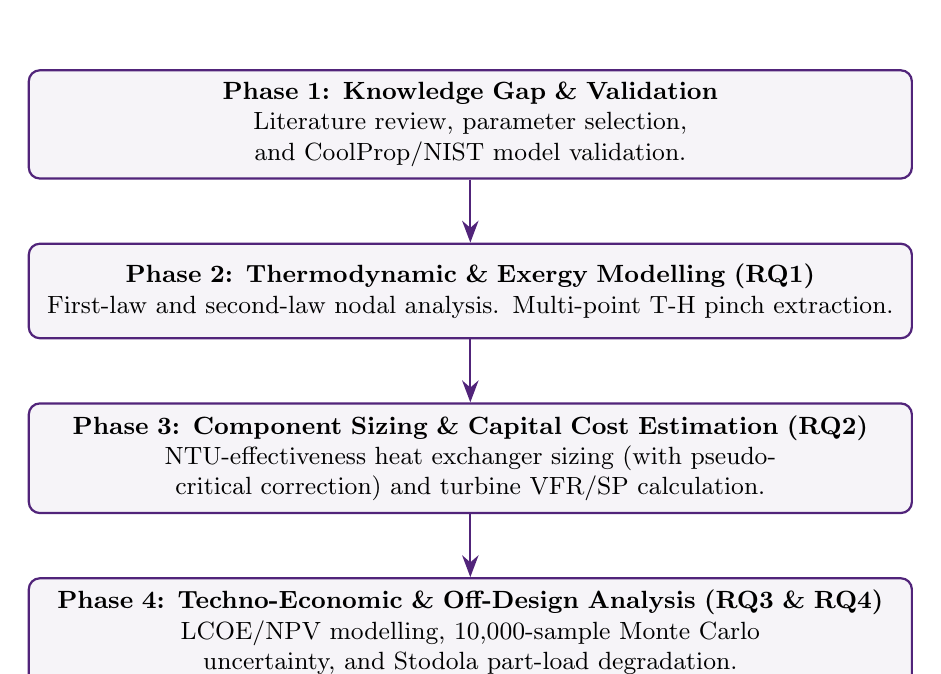
\begin{tikzpicture}[
    node distance=0.8cm,
    box/.style={rectangle, draw=uqpurple, fill=uqpurple!5, thick, rounded corners, text width=0.9\textwidth, minimum height=1.2cm, align=center, font=\small, inner sep=1ex},
    arrow/.style={-{Stealth[scale=1.2]}, thick, uqpurple}
]

\node[box] (lit) {\textbf{Phase 1: Knowledge Gap \& Validation} \\ Literature review, parameter selection, and CoolProp/NIST model validation.};

\node[box, below=of lit] (thermo) {\textbf{Phase 2: Thermodynamic \& Exergy Modelling (RQ1)} \\ First-law and second-law nodal analysis. Multi-point T-H pinch extraction.};

\node[box, below=of thermo] (sizing) {\textbf{Phase 3: Component Sizing \& Capital Cost Estimation (RQ2)} \\ NTU-effectiveness heat exchanger sizing (with pseudo-critical correction) and turbine VFR/SP calculation.};

\node[box, below=of sizing] (econ) {\textbf{Phase 4: Techno-Economic \& Off-Design Analysis (RQ3 \& RQ4)} \\ LCOE/NPV modelling, 10,000-sample Monte Carlo uncertainty, and Stodola part-load degradation.};

\draw[arrow] (lit) -- (thermo);
\draw[arrow] (thermo) -- (sizing);
\draw[arrow] (sizing) -- (econ);

\end{tikzpicture}
\caption{Overview of the interconnected four-phase methodology used to address RQ1--RQ4.}
\label{fig:methodology_flow}
\end{figure}

The research was structured in four phases corresponding to the four research
questions. The approach was set out in the thesis proposal, substantially
expanded in the Interim Report, and revised during the final modelling work
described here. Three revisions made after the Interim Report are material to
the results and are flagged where they arise: (i)~the recuperator energy
balance is limited by both streams (Section~\ref{sec:method_recup}), which
lowers the CO$_2$ cycle efficiencies reported at the interim stage;
(ii)~every primary heater is integrated with the waste-gas stream using a
duty-linear gas profile and a 10\,K approach (Section~\ref{sec:method_pinch});
and (iii)~the techno-economic comparison is made on a fixed-source basis
(Section~\ref{sec:method_rq3}).

\section{Phase 1 --- Literature Review}
\label{sec:method_lit}

A structured search was conducted across Scopus, Web of Science, and Google
Scholar following the PRISMA framework, covering WHR publications from 2005
to 2025 with five foundational pre-2005 sources included on merit (Dostal
2004; Short et al.\ 1995; Moran \& Shapiro 2018; Turton et al.\ 2012; Bell
et al.\ 2014). Coverage was organised around six themes: cycle thermodynamics
and variants; experimental and simulation performance data; transitional and
pseudo-critical CO$_2$ thermophysics; heat exchanger technology for
high-pressure CO$_2$; capital and operating cost data; and Australian
industrial waste heat availability. Thirty-two references were retained after
relevance screening; 29 are cited in the body of the thesis.

\section{Thermodynamic Modelling (RQ1)}
\label{sec:method_thermo}

\subsection{Cycle Architecture and State-Point Models}

Steady-state energy balance models for all three cycles were implemented in
Python\,3.9 using the CoolProp\,6.x library~\cite{Bell2014} for
thermodynamic property evaluation. The HEOS (Helmholtz Energy Equation of
State) backend was used throughout in preference to the default BICUBIC
interpolation because of its superior accuracy near the CO$_2$ critical
point, where the tCO$_2$ pump exit and the sCO$_2$ compressor inlet both
operate. At each state point four properties are extracted: specific enthalpy
($h$), specific entropy ($s$), density ($\rho$), and temperature ($T$).

Energy balances at each state point follow standard open-system forms. For
turbomachinery:
\begin{equation}
\dot{W} = \dot{m}(h_{in} - h_{out})
\label{eq:turbomachinery}
\end{equation}
For heat exchangers:
\begin{equation}
\dot{Q} = \dot{m}(h_{out} - h_{in})
\label{eq:hx}
\end{equation}
Isentropic efficiency is applied as:
\begin{equation}
h_{out} = h_{in} + \frac{h_{out,is} - h_{in}}{\eta_{is}}
\quad\text{(compression)}
\label{eq:compression}
\end{equation}
\begin{equation}
h_{out} = h_{in} - \eta_{is}(h_{in} - h_{out,is})
\quad\text{(expansion)}
\label{eq:expansion}
\end{equation}
Values of $\eta_{turbine} = 0.85$ and $\eta_{pump/compressor} = 0.80$ are
applied uniformly to all three cycles, ensuring genuine comparability. These
values are standard for preliminary analysis of small-to-medium scale
turbomachinery~\cite{Macchi2017} and represent a known simplification
addressed further in Section~\ref{sec:discussion_limitations}.

All heat exchangers and pipe runs are modelled as isobaric processes
($\Delta P = 0$) in the thermodynamic analysis phase. Real frictional pressure
drop --- particularly significant in CO$_2$ PCHEs --- is an identified
limitation acknowledged and quantified in Section~\ref{sec:discussion_limitations}.

\subsection{Cycle-Specific Parametric Assumptions}

The tCO$_2$ high-side pressure is scaled linearly from 12\,MPa at
150\,\textdegree C to 20\,MPa at 350\,\textdegree C and above, following
the optimal pressure relationship of Liu et al.~\cite{Liu2024}
($P_{high} = \min[20, \max(12,\, 8 + 0.048\,(T-100))]$\,MPa). Low-side
pressure is held at 5\,MPa for the baseline, corresponding to a condenser
temperature of 14.3\,\textdegree C. The recuperator effectiveness baseline is
$\varepsilon = 0.70$ for tCO$_2$ and $\varepsilon = 0.85$ for sCO$_2$.

\phantomsection\label{sec:method_recup}
The recuperator effectiveness is applied to the stream with the smaller
enthalpy capacity, so that neither stream can be driven past the inlet
temperature of the other:
\begin{equation}
Q_{recup} = \varepsilon \cdot \min\!\big[\,h_{cold}(T_{hot,in}) - h_{cold,in},\;
h_{hot,in} - h_{hot}(T_{cold,in})\,\big]
\label{eq:recup}
\end{equation}
This is the standard $\varepsilon$-NTU definition~\cite{Moran2018}. It
matters for CO$_2$ because $c_p$ differs strongly between the high- and
low-pressure sides near the critical point: at the CS2 condition the cold
(12.8\,MPa) side can absorb 251\,kJ/kg before reaching the turbine exhaust
temperature, whereas the hot (5\,MPa) side can release only 113\,kJ/kg before
reaching the pump exit temperature. Defining $\varepsilon$ on the cold side
alone, as was done in the Interim Report, transfers 176\,kJ/kg and drives the
hot stream to 14\,\textdegree C --- 10\,K \emph{below} the stream it is
heating --- which violates the second law. Equation~\eqref{eq:recup} is used
throughout this thesis, and the resulting efficiencies are lower than the
interim values (Section~\ref{sec:results_firstlaw}). The recuperator is also
discretised in 200 enthalpy steps to confirm that no internal temperature
crossover occurs (Section~\ref{sec:method_rq2}).

The sCO$_2$ cycle uses $P_{high} = 20$\,MPa and $P_{low} = 8$\,MPa, with
the compressor inlet set to $T_c + 5$\,K (35.98\,\textdegree C) to guarantee
operation in the supercritical region and maintain the near-critical
compressibility benefit.

In the parametric sweep the SRC uses $P_{high} = \min[10\,\text{MPa},\;
0.95 \times P_{sat}(T_{TIT})]$, i.e.\ the highest subcritical pressure that
leaves the turbine inlet slightly superheated, and $P_{low} = 10$\,kPa
(condenser temperature 45.8\,\textdegree C), a typical industrial condensing
pressure. This sweep characterises each cycle as a function of turbine inlet
temperature only; when the cycles are integrated with a real waste-gas stream
(Section~\ref{sec:method_rq2}) the steam pressure is instead chosen by the
boiler pinch constraint, which gives substantially lower pressures.

\subsection{Model Validation}

CoolProp outputs were cross-validated against NIST Webbook
data~\cite{Lemmon2018} at two SRC state points (Table~\ref{tab:validation}).
Both deviations lie well within the 1\,\% acceptance criterion. CoolProp
evaluates the CO$_2$ critical point as $T_c = 30.98$\,\textdegree C and
$P_c = 7.377$\,MPa, matching NIST REFPROP to within 0.04\,\%.

\begin{table}[H]
\centering
\caption{SRC model validation against NIST Webbook reference data.}
\label{tab:validation}
\renewcommand{\arraystretch}{1.2}
\begin{tabularx}{\textwidth}{>{\raggedright\arraybackslash}X
  >{\centering\arraybackslash}p{2.5cm}
  >{\centering\arraybackslash}p{2.5cm}
  >{\centering\arraybackslash}p{2.5cm}
  >{\centering\arraybackslash}p{2.0cm}}
\toprule
\rowcolor{tableheader}
\textbf{State point} & \textbf{NIST $h$} & \textbf{Model $h$} &
\textbf{NIST $s$} & \textbf{Deviation} \\
\rowcolor{tableheader}
& \textbf{(kJ/kg)} & \textbf{(kJ/kg)} & \textbf{(kJ/kg$\cdot$K)} & \\
\midrule
Saturated liquid, 10\,kPa & 191.83 & 191.81 & 0.6493 & 0.010\,\% \\
\rowcolor{rowgray}
Superheated steam, 400\,\textdegree C, 10\,MPa
& 3096.5 & 3097.45 & 6.2120 & 0.031\,\% \\
\bottomrule
\end{tabularx}
\end{table}

The global exergy balance (Eq.~\ref{eq:exergy_balance}) closes to machine
precision ($<10^{-12}$\,kJ/kg) for all three cycles, confirming internal
consistency of the second-law model.

\subsection{Parametric Sweep}

The primary sweep covers TIT from 150 to 600\,\textdegree C in
25\,\textdegree C steps. At each temperature, $\eta_{th}$, net specific
work, BWR, and exergy destruction by component are recorded. Separate sweeps
for recuperator effectiveness (Section~\ref{sec:method_sensitivity}) and
low-side pressure (Section~\ref{sec:method_sensitivity}) extend the analysis
beyond the single-parameter baseline.

\section{Exergy Analysis (RQ1)}
\label{sec:method_exergy}

An exergy balance is applied to every cycle component at a common turbine
inlet temperature of 400\,\textdegree C and at the three site design points
(Section~\ref{sec:method_rq2}). The dead state is $T_0 = 298.15$\,K,
$P_0 = 101.325$\,kPa (ASHRAE standard, confirmed with supervisor). Because
the three cycles circulate very different mass flows per unit of output,
component destruction is reported both per kilogram of working fluid and
per kilojoule of net work; only the latter is a like-for-like basis.

Specific flow exergy:
\begin{equation}
ex = (h - h_0) - T_0(s - s_0)
\label{eq:flow_exergy}
\end{equation}
For adiabatic turbomachinery:
\begin{equation}
\dot{E}_{x,dest} = T_0\,\dot{m}(s_{out} - s_{in})
\label{eq:adiabatic_exdest}
\end{equation}
For heat exchangers receiving heat from source at $T_{source}$:
\begin{align}
ex_{heat,in} &= Q_{in}\!\left(1 - \frac{T_0}{T_{source}}\right) \label{eq:exergy_heat}\\
\dot{E}_{x,dest,HX} &= ex_{heat,in} - (ex_{out} - ex_{in}) \label{eq:hx_exdest}
\end{align}
For condensers rejecting heat to environment:
\begin{equation}
\dot{E}_{x,dest,cond} = ex_{in} - ex_{out}
\label{eq:cond_exdest}
\end{equation}
Global balance closure check:
\begin{equation}
\dot{W}_{net} + \dot{E}_{x,dest,total} = ex_{heat,in}
\label{eq:exergy_balance}
\end{equation}

\section{Sensitivity Analysis (RQ1)}
\label{sec:method_sensitivity}

\subsection{Recuperator Effectiveness Sweep}

The tCO$_2$ cycle is evaluated at four recuperator effectiveness values
($\varepsilon = 0, 0.50, 0.70, 0.85$) at each of the three site design
points, with all other parameters held at baseline. For each $\varepsilon$
value the heater integration of Section~\ref{sec:method_pinch} is repeated to
determine how recuperation raises the heater inlet temperature and therefore
the lowest temperature to which the waste gas can be cooled. The quantity of
interest for waste heat recovery is not efficiency alone but the net work
obtained per kilogram of waste gas, $w_{gas} = \eta_{th}\,c_{p,gas}\,
(T_{src} - T_{gas,out})$, which combines both effects.

\subsection{Low-Side Pressure Sweep}

The tCO$_2$ cycle is evaluated at $P_{low} = 3.5, 4.0, 5.0, 6.0$ and
$7.0$\,MPa with $\varepsilon = 0.70$ fixed, at each site design point.
Condensing temperature, $\eta_{th}$, BWR, achievable gas outlet temperature
and $w_{gas}$ are recorded. The feasibility of each $P_{low}$ value is assessed
against the cooling-water temperatures available at the three Australian
sites, and the parasitic load of mechanical chilling, where it would be
required, is estimated from the condenser duty and a chiller coefficient of
performance of 4--6.
\section{Transitional Effects: Multi-Point T-H Heater Integration (RQ1/RQ2)}
\label{sec:method_pinch}

Following supervisor feedback to model transitional thermophysical effects,
the two-state-point energy balance of the primary heater is replaced by a
nodal integration along the exchanger. The working fluid is discretised in
200 equal enthalpy steps between the heater inlet and the turbine inlet, and
the temperature and $c_p$ are evaluated from real-fluid properties at every
node, which resolves the pseudo-critical peak. The same procedure is applied
to the steam boiler (where CoolProp returns the saturation temperature
through the two-phase region) and to the sCO$_2$ heater, so that all three
cycles are integrated with the waste-gas stream by one method.

The waste gas is treated as an ideal gas with constant $c_p$ in counter-flow.
Its temperature therefore falls \emph{linearly with heat duty}, not with
position or with node index:
\begin{equation}
T_{gas}(q) = T_{gas,out} + \left(T_{src} - T_{gas,out}\right)\frac{q}{Q}
\label{eq:gas_profile}
\end{equation}
where $q$ is the cumulative heat transferred from the cold end and $Q$ the
total heater duty per kilogram of working fluid. The distinction matters: a
profile that is linear in node index implicitly assumes the gas gives up equal
heat per node, which is false wherever the working fluid's $c_p$ varies. The
Interim Report used an index-linear profile, which produced a spurious
constant 10\,K difference along the whole heater; the corrected profile is
used here.

Two constraints close the problem. The turbine inlet is set 10\,K below the
source temperature (hot-end approach), and the gas outlet temperature is
found by bisection so that the minimum local temperature difference equals
the 10\,K approach:
\begin{equation}
\mathrm{PPTD} = \min_{i}\!\left[T_{gas,i} - T_{wf,i}\right] = 10\,\text{K}
\label{eq:pptd}
\end{equation}
This is the maximum heat that the stream can give up to that cycle. Because
the heater inlet temperature of the working fluid is the floor for the gas
outlet, a cycle whose heater inlet is hot (a recuperated sCO$_2$ cycle, for
example) can recover less of the stream than one whose heater inlet is cold.
The conductance is then accumulated segment by segment,
\begin{equation}
UA = \sum_{i} \frac{\Delta Q_i}{\mathrm{LMTD}_i}, \qquad
\mathrm{LMTD}_i = \frac{\Delta T_{i} - \Delta T_{i+1}}{\ln(\Delta T_{i}/\Delta T_{i+1})}
\label{eq:seg_UA}
\end{equation}
which is exact for counter-flow with piecewise-linear profiles. The two-point
LMTD result, $UA_{2pt} = Q/\mathrm{LMTD}(\Delta T_{cold},\Delta T_{hot})$, is
computed alongside for comparison (Section~\ref{sec:rq2_hx_sizing}).

\section{Equipment Sizing and Capital Cost (RQ2)}
\label{sec:method_rq2}

\subsection{Site Design Points}
\label{sec:method_sitedesign}

Each Australian site (Table~\ref{tab:casestudies}) is a fixed waste-gas
stream with source temperature $T_{src}$ and mass flow $\dot{m}_{gas}$. Each
cycle is integrated with the stream through the heater model of
Section~\ref{sec:method_pinch}. For the CO$_2$ cycles the pressures follow the
RQ1 rules. For the steam cycle the boiler pressure is a free design variable:
the evaporation temperature fixes an internal pinch at the start of boiling,
so a higher pressure raises cycle efficiency but prevents the gas from being
cooled as far. The pressure is therefore chosen by a golden-section search to
maximise the net work per kilogram of waste gas,
\begin{equation}
w_{gas} = \eta_{th}\; c_{p,gas}\,\left(T_{src} - T_{gas,out}\right),
\qquad \dot{W}_{site} = \dot{m}_{gas}\, w_{gas}
\label{eq:wgas}
\end{equation}
with $c_{p,gas} = 1.10$\,kJ/(kg$\cdot$K). Equation~\eqref{eq:wgas} is the
quantity a plant owner actually receives from a given stream; it rewards
both conversion efficiency and depth of heat recovery, and it is used
throughout RQ2--RQ4. The recuperator of each CO$_2$ cycle is discretised in
the same way as the heater (200 enthalpy steps with real properties on both
sides) to obtain its $UA$ and to check that no internal temperature crossover
occurs. The heat-rejection exchanger (condenser or gas cooler) is assigned a
mean temperature difference of 10\,K to the cooling medium for all three
cycles.

\subsection{Turbomachinery Compactness}

Turbine size parameter and volumetric flow ratio are calculated from
Macchi and Astolfi~\cite{Macchi2017}:
\begin{equation}
\mathrm{SP} = \frac{\dot{V}_{out}^{0.5}}{\Delta h_{is}^{0.25}}, \qquad
\mathrm{VFR} = \frac{v_{out}}{v_{in}}
\label{eq:sp_vfr}
\end{equation}
where $\dot{V}_{out}$ is the volumetric flow rate at turbine exhaust (m$^3$/s
per kg/s of working fluid) and $\Delta h_{is}$ is the isentropic enthalpy
drop (kJ/kg). A VFR below approximately 5 is taken as the threshold for
single-stage radial turbine feasibility~\cite{Macchi2017}. Both are evaluated
at the site design points.

\subsection{Heat Exchanger Area}

For the illustrative comparison of sizing methods, the tCO$_2$ heater area is
reported as $A = UA/U$ with the overall coefficient computed from the PCHE
resistance network
\begin{equation}
\frac{1}{U} = \frac{1}{h_{CO_2}} + \frac{t_{wall}}{k_{wall}} + \frac{1}{h_{gas}}
\label{eq:U_overall}
\end{equation}
with $h_{CO_2} = 2000$\,W/m$^2$K (supercritical CO$_2$ side, conservative
PCHE estimate from Dostal~\cite{Dostal2004}), $h_{gas} = 500$\,W/m$^2$K
(exhaust gas forced convection), $t_{wall} = 2$\,mm, and $k_{wall} =
15$\,W/mK (SS316), giving $U = 380$\,W/m$^2$K. The comparison is made at
$\varepsilon = 0$ (pump exit to turbine inlet), which places the
pseudo-critical $c_p$ peak inside the heater and maximises the divergence
between the segmented and two-point results. Capital costs are computed from
$UA$ directly, so the value of $U$ does not affect the economics.

\subsection{Capital Cost Estimation}
\label{sec:method_cost}

Every cycle is costed with the same method and the same correlations, applied
component by component to the site design point scaled to the required net
output (Table~\ref{tab:cost_basis}). CO$_2$ turbines and all heat exchangers
use the NETL correlations of Weiland, Lance and Pidaparti~\cite{Weiland2019};
the steam turbine uses a power law fitted to the US~DOE small-turbine
benchmarks~\cite{DOE2012}; pumps and the sCO$_2$ compressor use Turton et
al.~\cite{Turton2012}. Turbine cost is evaluated on \emph{shaft} power
($\dot{W}_{net}/(1-\mathrm{BWR})$), which penalises the high back-work ratio
of the sCO$_2$ cycle correctly. The condenser or cooler, omitted at the
interim stage, is included for all three cycles because low-efficiency WHR
plants reject three to six units of heat per unit of electricity.

\begin{table}[H]
\centering
\caption{Capital cost basis. All correlations escalated to 2026 by CEPCI
(2001: 397; 2012: 584.6; 2017: 567.5; 2026: $\approx$830~\cite{CEPCI2026})
and converted at 1\,USD = 1.395\,AUD~\cite{RBA2026}; +35\,\% installation on
all equipment~\cite{Turton2012}.}
\label{tab:cost_basis}
\renewcommand{\arraystretch}{1.3}
\small
\begin{tabularx}{\textwidth}{>{\raggedright\arraybackslash}p{3.0cm}
  >{\raggedright\arraybackslash}p{5.2cm}
  >{\raggedright\arraybackslash}p{2.6cm}
  >{\raggedright\arraybackslash}X}
\toprule
\rowcolor{tableheader}
\textbf{Component} & \textbf{Correlation (cost year)} & \textbf{Scaling variable} & \textbf{Validity / note} \\
\midrule
\rowcolor{rowgray}
Primary heater, recuperator & $49.45\,UA^{0.7544}\,f_T$ (2017)~\cite{Weiland2019} & $UA$ (W/K) & $1.6\times10^5$--$2.1\times10^8$\,W/K; $f_T=1$ below 550\,\textdegree C \\
Condenser / cooler & $32.88\,UA^{0.75}$ (2017)~\cite{Weiland2019} & $UA$ (W/K) & 10\,K mean $\Delta T$ assumed \\
\rowcolor{rowgray}
CO$_2$ turbine & $406{,}200\,\dot{W}_{sh}^{0.8}$ (2017)~\cite{Weiland2019} & shaft MW & 8--35\,MW; extrapolated below \\
Steam turbine & $a\,\dot{W}_{sh}^{\,b}$, fitted to USD\,900/kW at 150\,kW and USD\,200/kW at 2\,MW (2012)~\cite{DOE2012} & shaft kW & back-pressure benchmark; condensing units cost more \\
\rowcolor{rowgray}
sCO$_2$ compressor & Turton centrifugal compressor (2001)~\cite{Turton2012} & kW & 450--3000\,kW \\
Feed / CO$_2$ pump & Turton centrifugal pump (2001)~\cite{Turton2012} & kW & 1--300\,kW; no pressure factor \\
\rowcolor{rowgray}
Generator & $108{,}900\,\dot{W}_e^{0.5463}$ (2017)~\cite{Weiland2019} & MWe & 4--750\,MWe; extrapolated below \\
\bottomrule
\end{tabularx}
\end{table}

The Interim Report used ad hoc power-law coefficients for the turbines and
approximate terminal temperature differences for the heaters; those were
replaced because (i)~the coefficients could not be traced to the cited
source and (ii)~the terminal-difference approximation produced unphysical
driving forces for the steam boiler and the sCO$_2$ heater. Specific capital
cost (AUD/kW) is reported at 100\,kW, 500\,kW, 1\,MW and 5\,MW net output at
each site's design conditions, and the cost breakdown at 1\,MWe.

\section{Techno-Economic Analysis (RQ3)}
\label{sec:method_rq3}

\subsection{Case Study Definitions}

Three Australian industrial case studies are drawn from ARENA~\cite{ARENA2023}
and A2EP~\cite{A2EP2022} data (Table~\ref{tab:casestudies}).

\begin{table}[H]
\centering
\caption{Australian industrial case study definitions.}
\label{tab:casestudies}
\renewcommand{\arraystretch}{1.3}
\begin{tabularx}{\textwidth}{>{\raggedright\arraybackslash}p{1.3cm}
  >{\raggedright\arraybackslash}p{3.9cm}
  >{\centering\arraybackslash}p{1.6cm}
  >{\centering\arraybackslash}p{1.5cm}
  >{\centering\arraybackslash}p{1.9cm}
  >{\raggedright\arraybackslash}X}
\toprule
\rowcolor{tableheader}
\textbf{Case} & \textbf{Industry / Site} & \textbf{$T_{src}$ (\textdegree C)} &
\textbf{$\dot{m}_{gas}$ (kg/s)} & \textbf{Price (AUD/MWh)} & \textbf{Rationale} \\
\midrule
\rowcolor{rowgray}
CS2 & Gas processing intercooler (Pilbara, WA) & 200 & 30 & 130 &
  Representative LNG train; isolated-grid price premium~\cite{AEMO2024} \\
CS1 & Cement preheater exhaust (Gladstone, QLD) & 350 & 50 & 90 &
  Dominant WHR opportunity in Australian cement \\
\rowcolor{rowgray}
CS3 & Electric arc furnace flue gas (Sydney, NSW) & 500 & 20 & 100 &
  High-temperature WHR in NEM-connected steelmaking \\
\bottomrule
\end{tabularx}
\end{table}

\subsection{Fixed-Source Basis}

The comparison is made on a \emph{fixed-source} basis: each cycle is sized to
the net output it can recover from the site's stream
(Eq.~\ref{eq:wgas}), and its capital cost follows from the cost model at that
size. This is the decision an operator faces --- the stream is given, the
plant is not. A fixed-output comparison (all cycles at 1\,MWe) is reported in
RQ2 for the capital cost; on that basis, because waste heat is free and the
plant life and capacity factor are common, LCOE is simply proportional to the
specific capital cost, $\mathrm{LCOE} = (\mathrm{CRF} + 0.025)\,
\mathrm{TEC}/(8760\,\mathrm{CF})$, and adds no information beyond RQ2.

\subsection{LCOE, NPV, Payback and IRR}

Levelised Cost of Electricity is calculated following Short et
al.~\cite{Short1995}:
\begin{equation}
\mathrm{LCOE} = \frac{C_{cap} \cdot \mathrm{CRF} + C_{OM}}{E_{gen}}
\label{eq:lcoe}
\end{equation}
where $C_{cap}$ is the total erected cost (AUD), $C_{OM}$ is annual
operations and maintenance (2.5\,\% of capital per year, consistent with WHR
industry practice~\cite{Baglietto2023}), $E_{gen}$ is annual electricity
generation (MWh/yr at 85\,\% capacity factor), and CRF is the capital
recovery factor at a 7\,\% real discount rate over a 20-year project life:
\begin{equation}
\mathrm{CRF} = \frac{r(1+r)^n}{(1+r)^n - 1} = 0.0944
\label{eq:crf}
\end{equation}
Net present value is the sum of discounted annual net revenue (electricity
revenue minus O\&M) over the project life less the initial capital. Payback
is reported as \emph{discounted} payback --- the year in which cumulative
discounted net cash flow first exceeds the capital, interpolated within the
year --- so that it is consistent with NPV and LCOE; the simple payback is
also recorded. Internal rate of return is the discount rate at which NPV is
zero. Electricity prices are drawn from AEMO spot market data and WA
wholesale tariffs~\cite{AEMO2024} (Table~\ref{tab:casestudies}). Waste heat
is free, no carbon price is applied, and the cost of mechanical chilling for
the tCO$_2$ condenser is not included (Section~\ref{sec:plow_sensitivity}
quantifies it separately).

\subsection{Monte Carlo Uncertainty Analysis}

Uncertainty is quantified by 10,000-sample Monte Carlo, varying three
parameters simultaneously with uniform distributions: capital cost
($\pm 30$\,\%, matching the stated uncertainty of the cost correlations),
electricity price ($\pm 40$\,\%) and capacity factor (60--95\,\%). The
primary output is $P(\mathrm{NPV} > 0)$, with P10/P50/P90 values of NPV and
LCOE. A breakeven analysis also reports the reduction in heat exchanger cost
(primary heater plus recuperator) at which each CO$_2$ cycle would match the
best cycle's LCOE at the same site.

\section{Off-Design Analysis (RQ4)}
\label{sec:method_rq4}

Part-load performance is evaluated at five load levels --- 100, 80, 60, 40,
and 20\,\% of design mass flow --- using a simplified Stodola efficiency
correction:
\begin{equation}
\eta_{od} = \eta_0 \cdot [1 - 0.3(1-f)^2]
\label{eq:stodola}
\end{equation}
where $f$ is the part-load mass-flow fraction and the parabolic coefficient
$0.3$ is calibrated to Yang et al.'s~\cite{Yang2024} tCO$_2$ part-load data.
The correction is applied to the turbine of every cycle and additionally to
the sCO$_2$ compressor. Sliding-pressure control is applied: $P_{high} =
P_{design}\,f$ for the SRC, $P_{high} = 20\,(0.5 + 0.5f)$\,MPa for sCO$_2$
and $P_{high} = P_{design}\,(0.6 + 0.4f)$ for tCO$_2$, with low-side
pressures and turbine inlet temperature held at their site design values.
The heater integration is not re-solved at part load.

Operational flexibility is scored using the Marchionni et
al.~\cite{Marchionni2020} framework with four criteria: turndown ratio (weight
0.30), efficiency retention at 60\,\% load (0.30), efficiency retention at
40\,\% load (0.25), and startup complexity (0.15). Retention values are
averaged over the three sites. Startup complexity scores are assigned
qualitatively based on the literature: SRC 0.55 (steam drum pressurisation,
blow-down, long warm-up required); sCO$_2$ 0.75 (no phase change, faster
startup, critical control near compressor operating point); tCO$_2$ 0.80
(simplest startup, liquid pump, no near-critical compressor
management~\cite{Marchionni2020}).

\section{Implementation and Reproducibility}
\label{sec:method_code}

All models are implemented in a single Python package (\texttt{co2whr}) with
one script per research question and a driver (\texttt{run\_all.py}) that
regenerates every figure and every number in this thesis in under two minutes
(Appendix~\ref{app:code}). Results are written to a machine-readable file
(\texttt{results.json}) from which the tables in Chapters~\ref{ch:results_rq1}
to~\ref{ch:results_rq4} were transcribed.
%% ============================================================
%% CHAPTER 4 — RQ1: THERMODYNAMIC RESULTS
%% ============================================================
\chapter{Thermodynamic Performance Results (RQ1)}
\label{ch:results_rq1}

This chapter presents all results addressing RQ1. Section~\ref{sec:results_firstlaw}
covers first-law parametric performance; Section~\ref{sec:results_exergy} the
second-law exergy analysis; Section~\ref{sec:results_transitional} the
pseudo-critical heater integration; and Sections~\ref{sec:recup_sensitivity}
and~\ref{sec:plow_sensitivity} the recuperator and condensing-pressure
sensitivity sweeps, together with the warm-climate sensitivity of the sCO$_2$
compressor inlet. The thirteen findings of this chapter differ in several
respects from the Interim Report because of the recuperator correction
described in Section~\ref{sec:method_recup}; the differences are stated
explicitly where they arise.

\section{Model Validation}
\label{sec:results_validation}

SRC validation against NIST Webbook gave a maximum enthalpy deviation of
0.031\,\% (Table~\ref{tab:validation}), well inside the 1\,\% criterion.
CoolProp's CO$_2$ critical point ($T_c = 30.98$\,\textdegree C, $P_c =
7.377$\,MPa) matches NIST REFPROP to within 0.04\,\%. Physical
self-consistency checks at the SRC baseline (400\,\textdegree C TIT,
10\,MPa, 10\,kPa condenser) gave condenser temperature 45.8\,\textdegree C,
BWR 1.31\,\% and $\eta_{th}$ 32.79\,\%, all within expected ranges for
subcritical steam at this condition. The global exergy balance
(Eq.~\ref{eq:exergy_balance}) closes to machine precision for all three
cycles, and the discretised recuperator shows a positive temperature
difference at every node for every case reported (the smallest, 2.7\,K, is
the sCO$_2$ recuperator at the 200\,\textdegree C site, discussed in
Section~\ref{sec:rq2_sitedesign}).

\section{First-Law Parametric Performance}
\label{sec:results_firstlaw}

Figure~\ref{fig:threecycle} shows thermal efficiency and back-work ratio
across 150--600\,\textdegree C turbine inlet temperature for all three cycles
under the sweep rules of Section~\ref{sec:method_thermo}, and
Table~\ref{tab:rq1_results} extracts the values at the three Australian case
study temperatures.

\begin{figure}[H]
\centering
\thesisfig{RQ1_THREE_CYCLE.png}{0.92}{10cm}
\caption{Three-cycle thermal efficiency (top) and back-work ratio (bottom)
versus turbine inlet temperature, 150--600\,\textdegree C. Dashed lines mark
the Australian case study temperatures. Parameters: $\eta_{turbine} = 0.85$,
$\eta_{pump/comp} = 0.80$; SRC: $\le$10\,MPa, 10\,kPa condenser; sCO$_2$:
20/8\,MPa, $\varepsilon = 0.85$, compressor inlet 36\,\textdegree C; tCO$_2$:
$P_{high}(T)$, $P_{low} = 5$\,MPa, $\varepsilon = 0.70$. Recuperators limited
by both streams (Eq.~\ref{eq:recup}).}
\label{fig:threecycle}
\end{figure}

\begin{findingbox}
\textbf{Finding 1 --- Under the modelled assumptions the steam Rankine cycle
has the highest thermal efficiency at every turbine inlet temperature from
150 to 600\,\textdegree C.}
SRC rises from 19.06\,\% to 35.38\,\%; tCO$_2$ from 13.28\,\% to 30.12\,\%;
sCO$_2$ from 5.29\,\% to 30.09\,\%. The two CO$_2$ cycles converge on each
other at 600\,\textdegree C (\keyresult{30.1\,\% for both}) but remain
5.3~percentage points below steam. No crossover occurs within the WHR range.
This reverses the Interim Report's Findings~1 and~2 (sCO$_2$/SRC crossover at
362\,\textdegree C; tCO$_2$ ahead of SRC everywhere), both of which rested on
recuperators that transferred more heat than the hot stream could supply
(Section~\ref{sec:method_recup}). The steam figures are unchanged.
\end{findingbox}

\begin{findingbox}
\textbf{Finding 2 --- sCO$_2$ back-work ratio is prohibitive below
$\approx$300\,\textdegree C.}
At 150\,\textdegree C the compressor absorbs \keyresult{79.8\,\% of turbine
output}; at 200\,\textdegree C, 61.7\,\%; at 300\,\textdegree C, 45.0\,\%;
and still 26.9\,\% at 600\,\textdegree C. The tCO$_2$ pump absorbs 23.1\,\%
at 150\,\textdegree C (higher than the literature-reported 2--5\,\% owing to
$P_{low} = 5$\,MPa), falling to 12.4\,\% at 600\,\textdegree C. The SRC feed
pump stays below 1.5\,\% throughout. BWR, not turbine work, is why the
CO$_2$ cycles trail steam: the gross specific turbine work of the CO$_2$
cycles is comparable to steam per unit of heat input, but a quarter to
three-quarters of it is returned to the compressor.
\end{findingbox}

\begin{findingbox}
\textbf{Finding 3 --- The recuperator gain is bounded by the hot stream.}
With the effectiveness applied to the limiting stream, recuperation at
$\varepsilon = 0.70$ raises the tCO$_2$ efficiency by \keyresult{+3.4, +7.0
and +10.1 percentage points} at the 200, 350 and 500\,\textdegree C site
conditions (12.2$\to$15.7\,\%, 18.0$\to$25.0\,\%, 18.4$\to$28.5\,\%), compared
with the +12.3, +16.8 and +20.3 points obtained at the interim stage with a
cold-side-only effectiveness. The hot-side limit binds because the 5\,MPa
exhaust has a much smaller enthalpy capacity than the near-critical
high-pressure stream it heats.
\end{findingbox}

\begin{table}[H]
\centering
\caption{Thermal efficiency and back-work ratio at the Australian case study
turbine inlet temperatures (parametric sweep rules;
$\varepsilon_{sCO_2} = 0.85$, $\varepsilon_{tCO_2} = 0.70$, $P_{low,tCO_2} = 5$\,MPa).}
\label{tab:rq1_results}
\renewcommand{\arraystretch}{1.35}
\begin{tabularx}{\textwidth}{>{\raggedright\arraybackslash}p{3.8cm}
  >{\centering\arraybackslash}X >{\centering\arraybackslash}X >{\centering\arraybackslash}X}
\toprule
\rowcolor{tableheader}
\textbf{Parameter} &
\textbf{200\,\textdegree C (CS2)} &
\textbf{350\,\textdegree C (CS1)} &
\textbf{500\,\textdegree C (CS3)} \\
\midrule
\rowcolor{rowgray}
SRC $\eta_{th}$ (\%)     & 24.45 & 32.13 & 34.06 \\
sCO$_2$ $\eta_{th}$ (\%) & 12.53 & 22.70 & 27.84 \\
\rowcolor{rowgray}
tCO$_2$ $\eta_{th}$ (\%) & 16.09 & 25.28 & 28.66 \\
\midrule
SRC BWR (\%)              & 0.29  & 1.42  & 1.15 \\
\rowcolor{rowgray}
sCO$_2$ BWR (\%)         & 61.74 & 40.14 & 30.85 \\
tCO$_2$ BWR (\%)         & 19.98 & 18.56 & 14.22 \\
\midrule
\rowcolor{rowgray}
Best cycle ($\eta_{th}$) & SRC & SRC & SRC \\
\bottomrule
\end{tabularx}
\end{table}

\section{Second-Law Analysis}
\label{sec:results_exergy}

\subsection{Basis of Comparison}

Exergy destruction is conventionally tabulated per kilogram of working fluid.
For a comparison of cycles that is misleading, because at a common turbine
inlet temperature the three cycles circulate very different mass flows per
kilowatt: at 400\,\textdegree C the net specific work is 948\,kJ/kg for steam,
108\,kJ/kg for tCO$_2$ and 57\,kJ/kg for sCO$_2$. A kilogram of CO$_2$
destroys far less exergy than a kilogram of steam simply because it does far
less work. Figure~\ref{fig:exergy} therefore shows both bases, and
Table~\ref{tab:exergy} reports destruction per kilojoule of net work, which
is the like-for-like quantity. The Interim Report's statement that sCO$_2$
destroys 95\,\% less exergy than steam compared the per-kilogram totals and
is withdrawn.

\begin{figure}[H]
\centering
\thesisfig{RQ1_EXERGY.png}{1.0}{8cm}
\caption{Component exergy destruction at a common turbine inlet temperature of
400\,\textdegree C (dead state 25\,\textdegree C, 101.325\,kPa), per kilogram
of working fluid (left) and per kilojoule of net work (right). The right-hand
panel is the comparable basis.}
\label{fig:exergy}
\end{figure}

\begin{table}[H]
\centering
\caption{Exergy destruction at 400\,\textdegree C turbine inlet temperature,
in kJ per kJ of net work (per-kilogram totals in the last column).}
\label{tab:exergy}
\renewcommand{\arraystretch}{1.3}
\footnotesize
\begin{tabularx}{\textwidth}{>{\raggedright\arraybackslash}p{1.5cm}
  >{\centering\arraybackslash}X >{\centering\arraybackslash}X >{\centering\arraybackslash}X
  >{\centering\arraybackslash}X >{\centering\arraybackslash}X >{\centering\arraybackslash}p{1.3cm}
  >{\centering\arraybackslash}p{1.3cm} >{\centering\arraybackslash}p{1.7cm}}
\toprule
\rowcolor{tableheader}
\textbf{Cycle} & \textbf{Pump/ comp.} & \textbf{Heater} & \textbf{Turbine} &
\textbf{Cond./ cooler} & \textbf{Recup.} & \textbf{Total} & \textbf{$\eta_{ex}$ (\%)} & \textbf{Total (kJ/kg)} \\
\midrule
\rowcolor{rowgray}
SRC     & 0.002 & 0.396 & 0.167 & 0.134 & ---   & \textbf{0.699} & 58.9 & 663.2 \\
sCO$_2$ & 0.094 & 0.306 & 0.144 & 0.357 & 0.351 & \textbf{1.252} & 44.4 & 71.5 \\
\rowcolor{rowgray}
tCO$_2$ & 0.040 & 0.569 & 0.120 & 0.013 & 0.351 & \textbf{1.092} & 47.8 & 117.7 \\
\bottomrule
\end{tabularx}
\end{table}

\begin{findingbox}
\textbf{Finding 4 --- The steam boiler is the single largest loss in any
cycle, but per unit of work steam remains the most exergy-efficient cycle
at 400\,\textdegree C.}
The boiler destroys \keyresult{375\,kJ/kg, 56.6\,\% of all SRC losses},
because water evaporates at a fixed temperature well below the source. Yet
the SRC destroys only 0.70\,kJ of exergy per kJ of net work against 1.09 for
tCO$_2$ and 1.25 for sCO$_2$, with exergy efficiencies of 58.9, 47.8 and
44.4\,\%. The CO$_2$ cycles' non-isothermal heating does reduce heater
destruction per unit of work (0.31 for sCO$_2$ versus 0.40 for steam), but
the saving is more than consumed by their recuperators (0.35 each) and, for
sCO$_2$, by the compressor and gas cooler (0.09 and 0.36).
\end{findingbox}

\begin{findingbox}
\textbf{Finding 5 --- For the CO$_2$ cycles the recuperator, not the heater,
is the dominant internal irreversibility.}
At 400\,\textdegree C the recuperator accounts for 28\,\% of sCO$_2$
destruction and 32\,\% of tCO$_2$ destruction, as large as the heater in the
sCO$_2$ case. The large temperature differences that a fixed-effectiveness
recuperator tolerates when the two streams have very different $c_p$ are a
genuine second-law cost, and they grow with source temperature
(Section~\ref{sec:recup_sensitivity}).
\end{findingbox}

\subsection{Exergy at the Site Design Points}

Table~\ref{tab:exergy_sites} repeats the analysis at the three site design
points of Section~\ref{sec:rq2_sitedesign}, where the steam cycle operates at
the pinch-limited boiler pressure rather than at 10\,MPa. Two features stand
out. First, with a realistic boiler pressure the tCO$_2$ cycle is the most
exergy-efficient option at 200 and 350\,\textdegree C (42.4 and 47.9\,\%
against 39.0 and 45.4\,\% for steam), and steam leads only at 500\,\textdegree C.
Second, the tCO$_2$ condenser term is \emph{negative} at 200 and
350\,\textdegree C. The condenser rejects heat at 14.3\,\textdegree C, below
the 25\,\textdegree C dead state, so the condensate leaving it carries more
exergy (``cold exergy'') than the vapour entering. The balance closes only
because the model does not charge the cycle for the refrigeration needed to
supply a 14\,\textdegree C sink; that charge is quantified in
Section~\ref{sec:plow_sensitivity}.

\begin{table}[H]
\centering
\caption{Exergy destruction at the site design points (per kJ net work) with
the heat source treated as a reservoir at $T_{src}$.}
\label{tab:exergy_sites}
\renewcommand{\arraystretch}{1.3}
\footnotesize
\begin{tabularx}{\textwidth}{>{\raggedright\arraybackslash}p{1.0cm}>{\raggedright\arraybackslash}p{1.1cm}
  >{\centering\arraybackslash}X >{\centering\arraybackslash}X >{\centering\arraybackslash}X
  >{\centering\arraybackslash}X >{\centering\arraybackslash}X >{\centering\arraybackslash}X
  >{\centering\arraybackslash}p{1.2cm} >{\centering\arraybackslash}p{1.2cm}}
\toprule
\rowcolor{tableheader}
\textbf{Site} & \textbf{Cycle} & \textbf{Pump/ comp.} & \textbf{Heater} & \textbf{Turbine} &
\textbf{Cond./ cooler} & \textbf{Recup.} & \textbf{Total} & \textbf{$\eta_{th}$ (\%)} & \textbf{$\eta_{ex}$ (\%)} \\
\midrule
\rowcolor{rowgray} CS2 & SRC     & 0.000 & 1.010 & 0.165 & 0.387 & --- & 1.562 & 14.4 & 39.0 \\
                   CS2 & sCO$_2$ & 0.298 & 0.807 & 0.390 & 0.724 & 0.016 & 2.235 & 11.4 & 30.9 \\
\rowcolor{rowgray} CS2 & tCO$_2$ & 0.052 & 1.085 & 0.175 & $-$0.140 & 0.187 & 1.360 & 15.7 & 42.4 \\
\midrule
                   CS1 & SRC     & 0.000 & 0.828 & 0.165 & 0.210 & --- & 1.204 & 23.7 & 45.4 \\
\rowcolor{rowgray} CS1 & sCO$_2$ & 0.114 & 0.400 & 0.172 & 0.386 & 0.272 & 1.345 & 22.2 & 42.6 \\
                   CS1 & tCO$_2$ & 0.046 & 0.658 & 0.137 & $-$0.017 & 0.265 & 1.089 & 25.0 & 47.9 \\
\midrule
\rowcolor{rowgray} CS3 & SRC     & 0.001 & 0.681 & 0.166 & 0.146 & --- & 0.994 & 30.8 & 50.2 \\
                   CS3 & sCO$_2$ & 0.075 & 0.261 & 0.117 & 0.335 & 0.440 & 1.228 & 27.6 & 44.9 \\
\rowcolor{rowgray} CS3 & tCO$_2$ & 0.033 & 0.504 & 0.101 & 0.055 & 0.463 & 1.157 & 28.5 & 46.4 \\
\bottomrule
\end{tabularx}
\end{table}

\section{Transitional Effects: Pseudo-Critical Heater Integration}
\label{sec:results_transitional}

Figures~\ref{fig:pinch_200}--\ref{fig:pinch_500} show the tCO$_2$ heater T-h
diagrams at the three site conditions with $\varepsilon = 0$, so that the
pseudo-critical $c_p$ peak lies inside the heater, and
Table~\ref{tab:pinch} summarises the integration.

\begin{figure}[H]
\centering
\thesisfig{tco2_pinch_200C.png}{0.9}{9cm}
\caption{tCO$_2$ heater T-h diagram and $c_p$ profile for CS2 gas processing
(200\,\textdegree C source, 12.8\,MPa, $\varepsilon = 0$). Upper panel: CO$_2$
temperature (gold) and waste-gas temperature (red dashed, linear in heat
duty) versus cumulative heat transferred from the cold end. The approach of
10\,K is reached at \emph{both} terminals; the gap widens to 41.6\,K at a
CO$_2$ temperature of 88\,\textdegree C, just beyond the pseudo-critical
temperature of 57.1\,\textdegree C. Lower panel: $c_p$ along the heater, peak
4.42\,kJ/(kg$\cdot$K).}
\label{fig:pinch_200}
\end{figure}

\begin{figure}[H]
\centering
\thesisfig{tco2_pinch_350C.png}{0.9}{9cm}
\caption{tCO$_2$ heater T-h diagram and $c_p$ profile for CS1 cement
(350\,\textdegree C source, 20.0\,MPa, $\varepsilon = 0$). At 20\,MPa the $c_p$
peak is broader and lower (2.62\,kJ/(kg$\cdot$K) at 76\,\textdegree C); the
pump exit temperature rises to 32.1\,\textdegree C, so the gas cannot be
cooled below 42.1\,\textdegree C. Largest gap 49.0\,K at 145\,\textdegree C.}
\label{fig:pinch_350}
\end{figure}

\begin{figure}[H]
\centering
\thesisfig{tco2_pinch_500C.png}{0.9}{9cm}
\caption{tCO$_2$ heater T-h diagram and $c_p$ profile for CS3 steel
(500\,\textdegree C source, 20.0\,MPa, $\varepsilon = 0$). The large
source-to-sink span drives total heater duty to 701\,kJ/kg; largest gap
64.7\,K at 166\,\textdegree C.}
\label{fig:pinch_500}
\end{figure}

\begin{table}[H]
\centering
\caption{tCO$_2$ heater integration at $\varepsilon = 0$ (10\,K approach,
turbine inlet $T_{src} - 10$\,K) and the corresponding design values at
$\varepsilon = 0.70$.}
\label{tab:pinch}
\renewcommand{\arraystretch}{1.3}
\begin{tabularx}{\textwidth}{>{\raggedright\arraybackslash}p{6.2cm}
  >{\centering\arraybackslash}X >{\centering\arraybackslash}X >{\centering\arraybackslash}X}
\toprule
\rowcolor{tableheader}
\textbf{Parameter} & \textbf{CS2 (200\,\textdegree C)} & \textbf{CS1 (350\,\textdegree C)} & \textbf{CS3 (500\,\textdegree C)} \\
\midrule
\rowcolor{rowgray}
$P_{high}$ (MPa)                                 & 12.8  & 20.0  & 20.0 \\
Pump exit temperature (\textdegree C)            & 24.3  & 32.1  & 32.1 \\
\rowcolor{rowgray}
$T_{pc}$ (\textdegree C) / peak $c_p$ (kJ/kg$\cdot$K) & 57.1 / 4.42 & 76.2 / 2.62 & 75.8 / 2.62 \\
Gas outlet temperature, $\varepsilon = 0$ (\textdegree C) & 34.3 & 42.1 & 42.1 \\
\rowcolor{rowgray}
Heater duty, $\varepsilon = 0$ (kJ/kg)           & 360.5 & 517.3 & 701.3 \\
Minimum $\Delta T$ (K) and location              & 10.0, both ends & 10.0, both ends & 10.0, both ends \\
\rowcolor{rowgray}
Maximum $\Delta T$ (K) at $T_{CO_2}$ (\textdegree C) & 41.6 at 88 & 49.0 at 145 & 64.7 at 166 \\
Effective LMTD, segmented (K)                    & 22.9  & 27.1  & 32.3 \\
\midrule
\rowcolor{rowgray}
Heater inlet, $\varepsilon = 0.70$ (\textdegree C) & 50.2 & 91.1 & 141.1 \\
Gas outlet, $\varepsilon = 0.70$ (\textdegree C)  & 60.2 & 101.1 & 151.1 \\
\rowcolor{rowgray}
Effective LMTD, $\varepsilon = 0.70$ (K)          & 23.2 & 21.3 & 16.1 \\
\bottomrule
\end{tabularx}
\end{table}

\begin{findingbox}
\textbf{Finding 6 --- The tCO$_2$ heater is pinched at both terminals, and the
pseudo-critical $c_p$ peak opens the driving force in the middle rather than
closing it.}
With the gas profile linear in heat duty, the 10\,K approach is reached at
the cold end and at the hot end simultaneously, and the temperature
difference bulges to \keyresult{41.6, 49.0 and 64.7\,K} at CO$_2$ temperatures
of 88, 145 and 166\,\textdegree C, downstream of $T_{pc}$. The mechanism is
that CO$_2$ absorbs a large share of the duty while its temperature is still
low (high $c_p$), so its curve falls below the straight line joining its end
points while the gas, with constant $c_p$, follows that straight line. The
Interim Report's Finding~7 (``the pinch sits mid-exchanger at
129\,\textdegree C'') was an artefact of an index-linear gas profile that
produced a constant 10\,K gap everywhere, and is withdrawn.
\end{findingbox}

\begin{findingbox}
\textbf{Finding 7 --- The heater inlet temperature sets a hard floor on waste
heat recovery, and recuperation raises that floor.}
At $\varepsilon = 0$ the floor is the pump exit: the gas cannot leave below
\keyresult{34.3\,\textdegree C} at 12.8\,MPa or 42.1\,\textdegree C at
20\,MPa. At the design effectiveness of 0.70 the heater inlet rises to 50,
91 and 141\,\textdegree C and the gas can only be cooled to 60, 101 and
151\,\textdegree C. Recuperation therefore trades depth of heat recovery for
cycle efficiency, a trade quantified in Section~\ref{sec:recup_sensitivity}.
\end{findingbox}

\begin{findingbox}
\textbf{Finding 8 --- The pseudo-critical peak sharpens as pressure falls.}
At 12.8\,MPa, $T_{pc} = 57.1$\,\textdegree C with peak $c_p =
4.42$\,kJ/(kg$\cdot$K); at 20\,MPa, $T_{pc} = 76$\,\textdegree C with peak
$c_p = 2.62$\,kJ/(kg$\cdot$K). Lower pressure produces the more non-uniform
profile and therefore the larger departure between segmented and two-point
sizing, but the pump exit temperature is also lower, which deepens heat
recovery. The high-side pressure is thus a trade-off between heater
non-uniformity and recovery depth, in addition to its effect on efficiency.
\end{findingbox}

\section{Recuperator Sensitivity}
\label{sec:recup_sensitivity}

Figure~\ref{fig:recup_sensitivity} and Table~\ref{tab:recup} show the tCO$_2$
cycle at $\varepsilon = 0$, 0.50, 0.70 and 0.85 at each site design point.

\begin{figure}[H]
\centering
\thesisfig{RQ1_RECUPERATOR_SENSITIVITY.png}{1.0}{9cm}
\caption{tCO$_2$ recuperator effectiveness sensitivity at the three site design
points: thermal efficiency, net work per kilogram of waste gas, recuperator
duty and the achievable gas outlet temperature.}
\label{fig:recup_sensitivity}
\end{figure}

\begin{table}[H]
\centering
\caption{tCO$_2$ recuperator sensitivity ($P_{low} = 5$\,MPa, 10\,K approach).
$w_{gas}$ is the net work per kilogram of waste gas (Eq.~\ref{eq:wgas}).}
\label{tab:recup}
\renewcommand{\arraystretch}{1.25}
\footnotesize
\begin{tabularx}{\textwidth}{>{\raggedright\arraybackslash}p{1.0cm}>{\centering\arraybackslash}p{0.9cm}
  >{\centering\arraybackslash}X >{\centering\arraybackslash}X >{\centering\arraybackslash}X
  >{\centering\arraybackslash}X >{\centering\arraybackslash}X >{\centering\arraybackslash}X
  >{\centering\arraybackslash}p{1.6cm}}
\toprule
\rowcolor{tableheader}
\textbf{Site} & $\varepsilon$ & $\eta_{th}$ (\%) & BWR (\%) & $q_{in}$ (kJ/kg) & $Q_{recup}$ (kJ/kg) &
Heater inlet (\textdegree C) & Gas out (\textdegree C) & $w_{gas}$ (kJ/kg gas) \\
\midrule
\rowcolor{rowgray} CS2 & 0    & 12.23 & 20.69 & 360.5 & 0.0   & 24.3  & 34.3  & 22.30 \\
                   CS2 & 0.50 & 14.51 & 20.69 & 304.0 & 56.5  & 44.1  & 54.1  & 23.28 \\
\rowcolor{rowgray} CS2 & 0.70 & 15.67 & 20.69 & 281.4 & 79.1  & 50.2  & 60.2  & 24.10 \\
                   CS2 & 0.85 & 16.68 & 20.69 & 264.5 & 96.0  & 54.2  & 64.2  & 24.91 \\
\midrule
\rowcolor{rowgray} CS1 & 0    & 17.97 & 18.97 & 517.3 & 0.0   & 32.1  & 42.1  & 60.85 \\
                   CS1 & 0.50 & 22.47 & 18.97 & 413.7 & 103.6 & 75.0  & 85.0  & 65.49 \\
\rowcolor{rowgray} CS1 & 0.70 & 24.97 & 18.97 & 372.3 & 145.1 & 91.1  & 101.1 & 68.36 \\
                   CS1 & 0.85 & 27.25 & 18.97 & 341.2 & 176.2 & 104.2 & 114.2 & 70.68 \\
\midrule
\rowcolor{rowgray} CS3 & 0    & 18.39 & 14.44 & 701.3 & 0.0   & 32.1  & 42.1  & 92.60 \\
                   CS3 & 0.50 & 24.62 & 14.44 & 523.7 & 177.6 & 104.8 & 114.8 & 104.33 \\
\rowcolor{rowgray} CS3 & 0.70 & 28.49 & 14.44 & 452.7 & 248.7 & 141.1 & 151.1 & 109.32 \\
                   CS3 & 0.85 & 32.29 & 14.44 & 399.4 & 302.0 & 174.7 & 184.7 & 111.99 \\
\bottomrule
\end{tabularx}
\end{table}

\begin{findingbox}
\textbf{Finding 9 --- Recuperation improves efficiency far more than it
improves recovered work, because every increment of $\varepsilon$ raises the
gas outlet temperature.}
From $\varepsilon = 0$ to 0.85, $\eta_{th}$ rises by 4.5, 9.3 and
13.9~points at CS2, CS1 and CS3, but $w_{gas}$ rises by only
\keyresult{+12\,\%, +16\,\% and +21\,\%}, because the gas outlet temperature
climbs from 34--42\,\textdegree C to 64--185\,\textdegree C. The marginal
benefit also diminishes: the step 0.70$\to$0.85 adds 0.8--2.7\,kJ per
kilogram of gas while roughly doubling the recuperator conductance. BWR is
independent of $\varepsilon$ (20.7, 19.0 and 14.4\,\%), confirming that
recuperation reduces external heat input only and does not alter the pump or
turbine work.
\end{findingbox}

\begin{findingbox}
\textbf{Finding 10 --- At high effectiveness the recuperator approaches the
primary heater in duty, and at low source temperature it approaches the
10\,K approach limit.}
At $\varepsilon = 0.85$ the recuperator transfers 302\,kJ/kg at CS3, 76\,\%
of the external heat input (399\,kJ/kg). At CS2 the same effectiveness leaves
a minimum internal temperature difference of only \keyresult{9.8\,K},
essentially at the design approach, so $\varepsilon = 0.85$ is the practical
ceiling for a 200\,\textdegree C source at 12.8\,MPa. The baseline of 0.70
retains 21--86\,K of internal margin at all three sites.
\end{findingbox}

\section{Low-Side Pressure and Heat-Sink Sensitivity}
\label{sec:plow_sensitivity}

Figure~\ref{fig:plow_sensitivity} and Table~\ref{tab:plow} show the tCO$_2$
cycle at low-side pressures from 3.5 to 7.0\,MPa with $\varepsilon = 0.70$.

\begin{figure}[H]
\centering
\thesisfig{RQ1_PLOW_SENSITIVITY.png}{1.0}{7cm}
\caption{tCO$_2$ low-side pressure sensitivity ($\varepsilon = 0.70$):
condensing temperature, thermal efficiency and back-work ratio. The shaded
band marks the cooling-tower water temperatures typical of the three
Australian sites.}
\label{fig:plow_sensitivity}
\end{figure}

\begin{table}[H]
\centering
\caption{tCO$_2$ low-side pressure sensitivity ($\varepsilon = 0.70$, 10\,K
approach).}
\label{tab:plow}
\renewcommand{\arraystretch}{1.25}
\footnotesize
\begin{tabularx}{\textwidth}{>{\raggedright\arraybackslash}p{1.0cm}>{\centering\arraybackslash}p{1.3cm}
  >{\centering\arraybackslash}X >{\centering\arraybackslash}X >{\centering\arraybackslash}X
  >{\centering\arraybackslash}X >{\centering\arraybackslash}X >{\centering\arraybackslash}p{1.7cm}}
\toprule
\rowcolor{tableheader}
\textbf{Site} & $P_{low}$ (MPa) & $T_{cond}$ (\textdegree C) & $\eta_{th}$ (\%) & BWR (\%) & $w_{net}$ (kJ/kg) & Gas out (\textdegree C) & $w_{gas}$ (kJ/kg gas) \\
\midrule
\rowcolor{rowgray} CS2 & 3.5 & 0.2  & 18.47 & 16.72 & 61.6  & 44.7  & 31.56 \\
                   CS2 & 4.0 & 5.3  & 17.49 & 17.98 & 55.1  & 50.7  & 28.72 \\
\rowcolor{rowgray} CS2 & 5.0 & 14.3 & 15.67 & 20.69 & 44.1  & 60.2  & 24.10 \\
                   CS2 & 6.0 & 22.0 & 13.99 & 23.93 & 34.8  & 67.8  & 20.33 \\
\rowcolor{rowgray} CS2 & 7.0 & 28.7 & 12.36 & 28.88 & 26.3  & 76.5  & 16.80 \\
\midrule
                   CS1 & 3.5 & 0.2  & 27.59 & 15.59 & 117.5 & 80.4  & 81.82 \\
\rowcolor{rowgray} CS1 & 4.0 & 5.3  & 26.67 & 16.68 & 108.5 & 87.6  & 76.96 \\
                   CS1 & 5.0 & 14.3 & 24.97 & 18.97 & 93.0  & 101.1 & 68.36 \\
\rowcolor{rowgray} CS1 & 6.0 & 22.0 & 23.41 & 21.64 & 79.5  & 114.8 & 60.57 \\
                   CS1 & 7.0 & 28.7 & 21.91 & 25.55 & 67.0  & 131.0 & 52.79 \\
\midrule
\rowcolor{rowgray} CS3 & 3.5 & 0.2  & 31.56 & 11.84 & 161.5 & 120.2 & 131.86 \\
                   CS3 & 4.0 & 5.3  & 30.48 & 12.68 & 149.6 & 130.4 & 123.92 \\
\rowcolor{rowgray} CS3 & 5.0 & 14.3 & 28.49 & 14.44 & 129.0 & 151.1 & 109.32 \\
                   CS3 & 6.0 & 22.0 & 26.67 & 16.49 & 111.2 & 172.9 & 95.93 \\
\rowcolor{rowgray} CS3 & 7.0 & 28.7 & 24.95 & 19.49 & 94.9  & 197.7 & 82.97 \\
\bottomrule
\end{tabularx}
\end{table}

\begin{findingbox}
\textbf{Finding 11 --- The thermodynamically attractive condensing pressures
are climatically infeasible in Australia, and the 5\,MPa baseline is itself
marginal.}
$P_{low} = 3.5$\,MPa condenses at 0.2\,\textdegree C and 4.0\,MPa at
5.3\,\textdegree C --- unattainable at any of the three sites. The baseline
5\,MPa condenses at \keyresult{14.3\,\textdegree C}, which requires a sink
near 4\,\textdegree C for a 10\,K approach: colder than cooling-tower water
anywhere in Australia (typically 20--32\,\textdegree C~\cite{BOM2024}) and
achievable only with mechanical chilling. Only $P_{low} \ge 6.5$\,MPa
(condensing above 25\,\textdegree C) is compatible with evaporative cooling
at Gladstone or Sydney outside summer, and no subcritical pressure is
compatible with Pilbara summer conditions.
\end{findingbox}

\begin{findingbox}
\textbf{Finding 12 --- The cost of a cold sink would exceed the benefit of
the cycle at low source temperatures.}
If the 14.3\,\textdegree C condenser at 5\,MPa were served by an electric
chiller, the parasitic load would be $q_{out}/\mathrm{COP}$. With
$q_{out} = 237$, 279 and 324\,kJ/kg and $w_{net} = 44$, 93 and 129\,kJ/kg,
a chiller of COP~4 would consume \keyresult{134\,\%, 75\,\% and 63\,\%} of
the net output at CS2, CS1 and CS3 (90, 50 and 42\,\% at COP~6). Raising
$P_{low}$ to 7\,MPa (28.7\,\textdegree C) removes the need for chilling at
the cost of 3.1--3.5 efficiency points and 23--30\,\% of $w_{gas}$; at CS1
the resulting 52.8\,kJ per kilogram of gas equals that of the pinch-limited
steam cycle (Section~\ref{sec:rq2_sitedesign}).
\end{findingbox}

\begin{findingbox}
\textbf{Finding 13 --- The warm-climate penalty on sCO$_2$ is concentrated at
low source temperatures.}
Raising the compressor inlet from 32 to 40\,\textdegree C (8\,MPa) reduces
sCO$_2$ efficiency from \keyresult{15.7 to 9.2\,\%} at a 200\,\textdegree C
turbine inlet (a 42\,\% relative loss), from 23.6 to 21.3\,\% at
350\,\textdegree C, and from 28.0 to 27.1\,\% at 500\,\textdegree C. The
baseline of 36\,\textdegree C, chosen as 5\,K above the critical temperature
to guarantee single-phase compression with Australian cooling water, gives
12.5, 22.7 and 27.8\,\%. Near-critical compression is the source of the
sCO$_2$ cycle's advantage in the literature and it is exactly what a warm heat
sink takes away.
\end{findingbox}

\section{Comparison with Published Results}
\label{sec:lit_comparison}

Kizilkan~\cite{Kizilkan2020} reported 27.6\,\% for sCO$_2$ and 24.2\,\% for
steam at a 350\,\textdegree C cement source. The present steam value at the
350\,\textdegree C \emph{site design point} (pinch-limited to 0.91\,MPa,
Section~\ref{sec:rq2_sitedesign}) is 23.7\,\%, in close agreement; the
present sCO$_2$ value (22.2\,\% at the site, 22.7\,\% in the sweep) is lower
than Kizilkan's because his configuration is a recompression cycle with a
compressor inlet near 32\,\textdegree C, whereas this study models a simple
recuperated layout with a 36\,\textdegree C inlet and a hot-side-limited
recuperator. Jiang et al.~\cite{Jiang2023} found tCO$_2$ up to 5~points
ahead of sCO$_2$; this study finds tCO$_2$ ahead of sCO$_2$ by 2.6--3.6~points
between 200 and 350\,\textdegree C, narrowing to 0.8~points at
500\,\textdegree C, consistent in direction. Crespi et al.'s~\cite{Crespi2017}
40--50\,\% efficiencies for sCO$_2$ apply above 500\,\textdegree C with
optimised recompression layouts and cold sinks, conditions outside the WHR
range and the Australian climate considered here. The disagreement with the
literature is therefore not with the thermodynamics but with the boundary
conditions, and Findings~11--13 identify which ones.

\section{Summary of RQ1 Results}
\label{sec:rq1_summary}

Under consistent assumptions and a second-law-consistent recuperator, the
steam Rankine cycle has the highest thermal efficiency at every turbine inlet
temperature in the 150--600\,\textdegree C range; tCO$_2$ is second below
500\,\textdegree C and the two CO$_2$ cycles converge above it. Per unit of
net work the SRC is also the most exergy-efficient cycle at a common turbine
inlet temperature, although at realistic pinch-limited boiler pressures the
tCO$_2$ cycle leads at 200 and 350\,\textdegree C. The tCO$_2$ heater is
pinched at both terminals with the driving force widest in the middle, so
the transitional effect enlarges rather than restricts the mean temperature
difference. Recuperation raises efficiency but also the gas outlet
temperature, so it adds far less to the work recovered from a stream than to
the efficiency. Finally, the CO$_2$ cycles' sensitivity to the heat sink is
their defining weakness in Australia: the tCO$_2$ baseline needs a
14\,\textdegree C condenser that would cost more to provide than the cycle
produces at 200\,\textdegree C, and the sCO$_2$ cycle loses two-fifths of its
efficiency at 200\,\textdegree C if its compressor inlet warms from 32 to
40\,\textdegree C.
%% ============================================================
%% CHAPTER 5 — RQ2: SIZING AND CAPITAL COST
%% ============================================================
\chapter{Equipment Sizing and Capital Cost (RQ2)}
\label{ch:results_rq2}

This chapter answers RQ2 in four steps. Section~\ref{sec:rq2_sitedesign}
establishes the design point of each cycle at each site, including the
pinch-limited steam pressure and the power each cycle can recover from the
stream. Section~\ref{sec:rq2_sp_vfr} compares turbine compactness,
Section~\ref{sec:rq2_hx_sizing} compares heat exchanger sizing methods, and
Section~\ref{sec:rq2_capital} reports capital cost versus plant size and its
breakdown by component.

\section{Site Design Points}
\label{sec:rq2_sitedesign}

Table~\ref{tab:sitedesign} gives the design point of every cycle at every
site after integration with the waste-gas stream
(Section~\ref{sec:method_sitedesign}). Two numbers in each row matter more
than the efficiency: the gas outlet temperature, which fixes how much of the
stream is used, and $w_{gas}$, the net work obtained per kilogram of gas.

\begin{table}[H]
\centering
\caption{Site design points (turbine inlet $T_{src}-10$\,K, 10\,K heater
approach). $T^{*}$ is the saturation temperature of the steam boiler (s), the
sCO$_2$ compressor inlet temperature (i) or the tCO$_2$ condensing
temperature (c). $w_{gas}$ is the net work per kilogram of waste gas and
$\dot{W}_{site}$ the net output from the whole stream of
Table~\ref{tab:casestudies}.}
\label{tab:sitedesign}
\renewcommand{\arraystretch}{1.25}
\footnotesize
\begin{tabular}{@{}l l r r r r r r r r@{}}
\toprule
\rowcolor{tableheader}
\textbf{Site} & \textbf{Cycle} & $P_{high}$ & $T^{*}$ & $\eta_{th}$ & BWR & Heater in & Gas out & $w_{gas}$ & $\dot{W}_{site}$ \\
\rowcolor{tableheader}
 & & (MPa) & (\textdegree C) & (\%) & (\%) & (\textdegree C) & (\textdegree C) & (kJ/kg) & (kW) \\
\midrule
\rowcolor{rowgray} CS2 & SRC     & 0.16 & 113.1\,s & 14.44 & 0.0  & 45.8  & 113.6 & 13.7 & 412 \\
                   CS2 & sCO$_2$ & 20.0 & 36.0\,i  & 11.43 & 64.4 & 100.0 & 110.0 & 11.3 & 340 \\
\rowcolor{rowgray} CS2 & tCO$_2$ & 12.8 & 14.3\,c  & 15.67 & 20.7 & 50.2  & 60.2  & 24.1 & \textbf{723} \\
\midrule
                   CS1 & SRC     & 0.91 & 175.9\,s & 23.67 & 0.2  & 45.9  & 147.2 & 52.8 & 2639 \\
\rowcolor{rowgray} CS1 & sCO$_2$ & 20.0 & 36.0\,i  & 22.24 & 41.0 & 177.5 & 187.5 & 39.8 & 1988 \\
                   CS1 & tCO$_2$ & 20.0 & 14.3\,c  & 24.97 & 19.0 & 91.1  & 101.1 & 68.4 & \textbf{3418} \\
\midrule
\rowcolor{rowgray} CS3 & SRC     & 3.69 & 245.7\,s & 30.82 & 0.5  & 46.2  & 164.7 & 113.7 & \textbf{2273} \\
                   CS3 & sCO$_2$ & 20.0 & 36.0\,i  & 27.58 & 31.3 & 279.0 & 289.1 & 64.0 & 1280 \\
\rowcolor{rowgray} CS3 & tCO$_2$ & 20.0 & 14.3\,c  & 28.49 & 14.4 & 141.1 & 151.1 & 109.3 & 2186 \\
\bottomrule
\end{tabular}
\end{table}

\begin{findingbox}
\textbf{Finding 14 --- Integrated with a real stream, the steam cycle must run
at a far lower pressure than the parametric sweep suggests.}
The boiler pinch at the start of evaporation limits the optimum pressure to
\keyresult{0.16, 0.91 and 3.69\,MPa} at the 200, 350 and 500\,\textdegree C
sites (saturation 113, 176 and 246\,\textdegree C), giving site efficiencies
of 14.4, 23.7 and 30.8\,\% against 24.5, 32.1 and 34.1\,\% in the sweep. A
higher pressure raises efficiency but forces the gas to leave hotter, and the
product $\eta_{th}(T_{src}-T_{gas,out})$ peaks at these values. Any
comparison that evaluates steam at 10\,MPa against a 200--350\,\textdegree C
exhaust stream overstates it badly.
\end{findingbox}

\begin{findingbox}
\textbf{Finding 15 --- On a fixed-source basis the tCO$_2$ cycle recovers the
most power at 200 and 350\,\textdegree C, and the sCO$_2$ cycle the least at
every site.}
From the CS2 stream tCO$_2$ delivers \keyresult{723\,kW against 412\,kW for
steam and 340\,kW for sCO$_2$}; from CS1, 3418 against 2639 and 1988\,kW;
from CS3, 2186 against 2273 and 1280\,kW. The ranking follows the gas outlet
temperature, not the efficiency: tCO$_2$ cools the gas to 60--151\,\textdegree C
because its heater inlet is the recuperator outlet at 50--141\,\textdegree C;
steam cools it to 114--165\,\textdegree C, limited by the evaporator pinch;
the recuperated sCO$_2$ cycle cools it only to 110--289\,\textdegree C because
its heater inlet is 100--279\,\textdegree C. At CS3 the sCO$_2$ cycle uses
only 63\,\% of the heat that steam uses. The sCO$_2$ recuperator at CS2 also
reaches an internal temperature difference of 2.7\,K, below the 10\,K design
approach, so that design point is not practically realisable without a lower
effectiveness.
\end{findingbox}

\section{Turbine Compactness: Size Parameter and Volumetric Flow Ratio}
\label{sec:rq2_sp_vfr}

Figure~\ref{fig:sp_vfr} and Table~\ref{tab:sp_vfr} compare turbine size
parameter and volumetric flow ratio at the site design points.

\begin{figure}[H]
\centering
\thesisfig{RQ2_TURBINE_SP_VFR.png}{1.0}{8cm}
\caption{Turbine size parameter (left) and volumetric flow ratio (right, log
scale) at the site design points. VFR $< 5$ permits a single-stage radial
turbine.}
\label{fig:sp_vfr}
\end{figure}

\begin{table}[H]
\centering
\caption{Turbine size parameter (per kg/s) and volumetric flow ratio at the site
design points.}
\label{tab:sp_vfr}
\renewcommand{\arraystretch}{1.3}
\begin{tabularx}{\textwidth}{>{\raggedright\arraybackslash}p{3.6cm}
  >{\centering\arraybackslash}X >{\centering\arraybackslash}X >{\centering\arraybackslash}X}
\toprule
\rowcolor{tableheader}
\textbf{Parameter} & \textbf{CS2 (200\,\textdegree C)} & \textbf{CS1 (350\,\textdegree C)} & \textbf{CS3 (500\,\textdegree C)} \\
\midrule
\rowcolor{rowgray}
SP, SRC (m$\cdot$(kJ/kg)$^{-0.25}$)     & 0.810 & 0.694 & 0.632 \\
SP, sCO$_2$                              & 0.031 & 0.035 & 0.038 \\
\rowcolor{rowgray}
SP, tCO$_2$                              & 0.040 & 0.039 & 0.042 \\
SP ratio SRC/sCO$_2$, SRC/tCO$_2$        & 26, 20 & 20, 18 & 17, 15 \\
\midrule
\rowcolor{rowgray}
VFR, SRC                                 & 10.5 & 45.2 & 148 \\
VFR, sCO$_2$                             & 2.01 & 2.08 & 2.11 \\
\rowcolor{rowgray}
VFR, tCO$_2$                             & 2.14 & 3.08 & 3.13 \\
\bottomrule
\end{tabularx}
\end{table}

\begin{findingbox}
\textbf{Finding 16 --- CO$_2$ turbines are 15--26 times more compact than the
steam turbine at the same site.}
The size parameter of the steam turbine is 0.63--0.81\,m$\cdot$(kJ/kg)$^{-0.25}$
per kg/s against 0.031--0.042 for the CO$_2$ cycles; the ratio is largest at
the lowest source temperature (\keyresult{26$\times$ at CS2}) because the
low-pressure steam cycle there exhausts a very large specific volume. sCO$_2$
is 11--29\,\% more compact than tCO$_2$, a gap that narrows with temperature.
\end{findingbox}

\begin{findingbox}
\textbf{Finding 17 --- The steam turbine needs a multi-stage machine at
350\,\textdegree C and above; both CO$_2$ cycles stay single-stage.}
Steam VFR is 10.5, 45 and 148 at the three site pressures (lower than the
89--807 of the 10\,MPa sweep because the site pressures are lower), all above
the single-stage threshold of 5. CO$_2$ VFR is \keyresult{2.0--3.1} at every
site. Compactness is the CO$_2$ cycles' most robust advantage; it survives
every other correction made in this thesis.
\end{findingbox}

\section{Heat Exchanger Sizing: Segmented versus Two-Point LMTD}
\label{sec:rq2_hx_sizing}

Figure~\ref{fig:hx_ntu_lmtd} compares the tCO$_2$ heater area from the
segmented integration (Eq.~\ref{eq:seg_UA}) with the two-point LMTD result at
$\varepsilon = 0$, using $U = 380$\,W/m$^2$K.

\begin{figure}[H]
\centering
\thesisfig{RQ2_HX_AREA_NTU_vs_LMTD.png}{1.0}{8cm}
\caption{tCO$_2$ heater area at $\varepsilon = 0$: segmented 200-node
integration versus two-point LMTD (left), and the percentage by which the
two-point method overestimates the area (right).}
\label{fig:hx_ntu_lmtd}
\end{figure}

\begin{findingbox}
\textbf{Finding 18 --- Two-point LMTD overestimates the tCO$_2$ heater area by
129--223\,\% when the pseudo-critical peak lies inside the heater.}
Segmented areas are 41.5, 50.2 and 57.2\,m$^2$ per kg/s against 94.9, 136.2
and 184.7\,m$^2$ from the two-point method (\keyresult{+129, +171 and
+223\,\%}). Because both terminals sit at the 10\,K approach
(Finding~6), the two-point LMTD is exactly 10\,K, whereas the duty-weighted
mean driving force is 22.9, 27.1 and 32.3\,K. The error grows with source
temperature because the mid-exchanger bulge grows. A designer using the
two-point method would price the tCO$_2$ heater at two to three times its
true cost. At the design effectiveness of 0.70 the heater inlet lies above
$T_{pc}$, the profile is nearly linear and the two methods agree to within
a few per cent; the capital costs that follow use the segmented $UA$ in all
cases.
\end{findingbox}

\section{Capital Cost Estimation}
\label{sec:rq2_capital}

Figure~\ref{fig:capital_cost} shows specific capital cost against plant size
at each site's design conditions, and Figure~\ref{fig:cost_breakdown} and
Table~\ref{tab:cost_breakdown} the breakdown at 1\,MWe. All three cycles are
costed with the correlations of Table~\ref{tab:cost_basis}.

\begin{figure}[H]
\centering
\thesisfig{RQ2_CAPITAL_COST_AUD_per_kW.png}{1.0}{7cm}
\caption{Total erected cost per kilowatt (2026 AUD) versus net output at the
three site design conditions.}
\label{fig:capital_cost}
\end{figure}

\begin{table}[H]
\centering
\caption{Specific capital cost (total erected, AUD/kW, 2026) versus net
output.}
\label{tab:capital}
\renewcommand{\arraystretch}{1.25}
\begin{tabularx}{\textwidth}{>{\raggedright\arraybackslash}p{1.0cm}>{\raggedright\arraybackslash}p{1.3cm}
  >{\centering\arraybackslash}X >{\centering\arraybackslash}X >{\centering\arraybackslash}X >{\centering\arraybackslash}X}
\toprule
\rowcolor{tableheader}
\textbf{Site} & \textbf{Cycle} & \textbf{100\,kW} & \textbf{500\,kW} & \textbf{1\,MW} & \textbf{5\,MW} \\
\midrule
\rowcolor{rowgray} CS2 & SRC     & 9{,}900  & 5{,}587  & \textbf{4{,}444} & 2{,}698 \\
                   CS2 & sCO$_2$ & 20{,}126 & 13{,}798 & 11{,}626 & 7{,}670 \\
\rowcolor{rowgray} CS2 & tCO$_2$ & 10{,}308 & 6{,}838  & 5{,}757  & 3{,}899 \\
\midrule
                   CS1 & SRC     & 7{,}469  & 3{,}956  & \textbf{3{,}071} & 1{,}776 \\
\rowcolor{rowgray} CS1 & sCO$_2$ & 11{,}953 & 8{,}226  & 6{,}971  & 4{,}676 \\
                   CS1 & tCO$_2$ & 7{,}951  & 5{,}253  & 4{,}421  & 2{,}998 \\
\midrule
\rowcolor{rowgray} CS3 & SRC     & 6{,}630  & 3{,}394  & \textbf{2{,}598} & 1{,}459 \\
                   CS3 & sCO$_2$ & 10{,}366 & 7{,}110  & 6{,}031  & 4{,}069 \\
\rowcolor{rowgray} CS3 & tCO$_2$ & 7{,}728  & 5{,}098  & 4{,}286  & 2{,}897 \\
\bottomrule
\end{tabularx}
\end{table}

\begin{figure}[H]
\centering
\thesisfig{RQ2_COST_BREAKDOWN.png}{1.0}{7cm}
\caption{Capital cost breakdown at 1\,MWe net output (installed basis, 2026
AUD).}
\label{fig:cost_breakdown}
\end{figure}

\begin{table}[H]
\centering
\caption{Equipment cost breakdown at 1\,MWe (kAUD, 2026, before the 35\,\%
installation factor) and the turbine and compression shaft powers behind it.}
\label{tab:cost_breakdown}
\renewcommand{\arraystretch}{1.25}
\footnotesize
\begin{tabularx}{\textwidth}{>{\raggedright\arraybackslash}p{0.9cm}>{\raggedright\arraybackslash}p{1.0cm}
  >{\centering\arraybackslash}X >{\centering\arraybackslash}X >{\centering\arraybackslash}X >{\centering\arraybackslash}X
  >{\centering\arraybackslash}X >{\centering\arraybackslash}X >{\centering\arraybackslash}p{1.2cm} >{\centering\arraybackslash}p{1.3cm}}
\toprule
\rowcolor{tableheader}
\textbf{Site} & \textbf{Cycle} & Turbine & Pump/ comp. & Heater & Recup. & Cooler & Gen. & \textbf{Total} & Shaft kW (turb./comp.) \\
\midrule
\rowcolor{rowgray} CS2 & SRC     & 593  & 7    & 1037 & ---  & 1433 & 222 & 3292 & 1000 / 0 \\
                   CS2 & sCO$_2$ & 1896 & 1250 & 2433 & 1059 & 1752 & 222 & 8612 & 2813 / 1813 \\
\rowcolor{rowgray} CS2 & tCO$_2$ & 998  & 76   & 1280 & 356  & 1333 & 222 & 4265 & 1261 / 261 \\
\midrule
                   CS1 & SRC     & 593  & 7    & 544  & ---  & 908  & 222 & 2275 & 1002 / 2 \\
\rowcolor{rowgray} CS1 & sCO$_2$ & 1264 & 619  & 1605 & 489  & 964  & 222 & 5164 & 1695 / 695 \\
                   CS1 & tCO$_2$ & 981  & 70   & 960  & 181  & 861  & 222 & 3275 & 1234 / 234 \\
\midrule
\rowcolor{rowgray} CS3 & SRC     & 594  & 9    & 408  & ---  & 692  & 222 & 1924 & 1005 / 5 \\
                   CS3 & sCO$_2$ & 1119 & 442  & 1542 & 363  & 778  & 222 & 4467 & 1456 / 456 \\
\rowcolor{rowgray} CS3 & tCO$_2$ & 939  & 54   & 1073 & 135  & 752  & 222 & 3175 & 1169 / 169 \\
\bottomrule
\end{tabularx}
\end{table}

\begin{findingbox}
\textbf{Finding 19 --- At equal output the steam cycle is the cheapest to
build at every site, tCO$_2$ costs 30--65\,\% more and sCO$_2$ two to three
times more.}
At 1\,MWe the total erected cost is \keyresult{AUD\,4{,}444, 3{,}071 and
2{,}598/kW} for steam at CS2, CS1 and CS3; 5{,}757, 4{,}421 and 4{,}286/kW for
tCO$_2$; and 11{,}626, 6{,}971 and 6{,}031/kW for sCO$_2$. Specific cost
falls by 61--78\,\% between 100\,kW and 5\,MW, and the ordering is the same at
every size. The Interim Report's result that sCO$_2$ was the cheapest cycle
at 200 and 350\,\textdegree C arose from a sign error in its heater
temperature difference that priced the sCO$_2$ heater at a few per cent of
its true cost, and is withdrawn.
\end{findingbox}

\begin{findingbox}
\textbf{Finding 20 --- The sCO$_2$ cost penalty is turbomachinery: a high
back-work ratio means every kilowatt of net output needs several kilowatts
of machinery.}
At CS2 a 1\,MWe sCO$_2$ plant needs a \keyresult{2.8\,MW turbine and a
1.8\,MW compressor}; turbomachinery is 37\,\% of its equipment cost against
25\,\% for tCO$_2$ and 18\,\% for steam. The CO$_2$ turbine is also costed on
a correlation (Weiland et al.) whose data begin at 8\,MW and which gives a
higher unit cost than the steam benchmark at 1\,MW (USD\,594/kW against
425/kW), reflecting the immaturity of small high-pressure CO$_2$ machines.
\end{findingbox}

\begin{findingbox}
\textbf{Finding 21 --- Heat exchangers are 35--43\,\% of CO$_2$ equipment cost,
and heat rejection is a large cost for every cycle at low source
temperature.}
The primary heater plus recuperator account for 35--43\,\% of CO$_2$
equipment cost and 21--32\,\% of the steam cycle's. The condenser or cooler,
omitted at the interim stage, is \keyresult{17--44\,\%} of equipment cost:
largest for the 14\,\%-efficient steam cycle at CS2, which rejects six units
of heat per unit of electricity, and smallest for the sCO$_2$ cycle at CS3.
A low-grade WHR plant is, in capital terms, mostly heat exchangers.
\end{findingbox}

\section{Summary of RQ2 Results}
\label{sec:rq2_summary}

Integrating each cycle with the actual waste-gas stream changes the picture
drawn by the parametric sweep. The steam cycle must run at 0.16--3.7\,MPa
rather than 10\,MPa, which lowers its efficiency to 14--31\,\% but still
leaves it the cheapest plant per kilowatt at every site, 30--65\,\% below
tCO$_2$ and a factor of two to three below sCO$_2$. The tCO$_2$ cycle,
however, recovers 29\,\% more power than steam from the 350\,\textdegree C
stream and 75\,\% more from the 200\,\textdegree C stream, because its cold
heater inlet lets it cool the gas further. The sCO$_2$ cycle is penalised
twice: its hot recuperated heater inlet leaves most of the stream unused,
and its back-work ratio makes its turbomachinery the most expensive of the
three. The CO$_2$ cycles' compactness advantage (15--26$\times$ in size
parameter) is unaffected by any of these corrections. Which of these effects
dominates the economics is the subject of RQ3.
%% ============================================================
%% CHAPTER 6 — RQ3: TECHNO-ECONOMICS
%% ============================================================
\chapter{Techno-Economic Analysis (RQ3)}
\label{ch:results_rq3}

This chapter answers RQ3 on the fixed-source basis of
Section~\ref{sec:method_rq3}: each cycle is sized to the output it can
recover from the site stream (Table~\ref{tab:sitedesign}), costed at that
size, and evaluated at the site electricity price.
Section~\ref{sec:rq3_deterministic} gives the deterministic results,
Section~\ref{sec:rq3_recovery} examines why the ranking differs from the
efficiency ranking, Section~\ref{sec:rq3_montecarlo} the Monte Carlo
robustness and breakeven analysis.

\section{Deterministic LCOE, NPV, Payback and IRR}
\label{sec:rq3_deterministic}

\begin{figure}[H]
\centering
\thesisfig{RQ3_LCOE_NPV_MONTE_CARLO.png}{1.0}{10cm}
\caption{Techno-economic results on a fixed-source basis (2026 AUD): net
power recovered from each stream, LCOE against the site electricity price,
project NPV, and Monte Carlo probability of positive NPV.}
\label{fig:rq3_results}
\end{figure}

\begin{table}[H]
\centering
\caption{Deterministic techno-economic results on a fixed-source basis
(7\,\% real discount rate, 20-year life, 85\,\% capacity factor, O\&M 2.5\,\%
of capital). Payback is discounted.}
\label{tab:rq3_results}
\renewcommand{\arraystretch}{1.25}
\footnotesize
\begin{tabularx}{\textwidth}{>{\raggedright\arraybackslash}p{0.9cm}>{\raggedright\arraybackslash}p{1.0cm}
  >{\centering\arraybackslash}X >{\centering\arraybackslash}X >{\centering\arraybackslash}X
  >{\centering\arraybackslash}X >{\centering\arraybackslash}X >{\centering\arraybackslash}X >{\centering\arraybackslash}X}
\toprule
\rowcolor{tableheader}
\textbf{Site} & \textbf{Cycle} & Output (kW) & TEC (kAUD) & TEC (AUD/kW) & LCOE (AUD/MWh) & NPV (kAUD) & Payback (yr) & IRR (\%) \\
\midrule
\rowcolor{rowgray} CS2 & SRC     & 412  & 2{,}457  & 5{,}967  & \textbf{95.7}  & 1{,}115  & 10.6 & 12.4 \\
                   CS2 & sCO$_2$ & 340  & 5{,}144  & 15{,}146 & 242.9 & $-$3{,}023 & never & $-$2.3 \\
\rowcolor{rowgray} CS2 & tCO$_2$ & 723  & 4{,}511  & 6{,}238  & 100.0 & \textbf{1{,}710} & 11.4 & 11.6 \\
\midrule
                   CS1 & SRC     & 2639 & 5{,}790  & 2{,}194  & \textbf{35.2}  & \textbf{11{,}415} & 4.2 & 27.8 \\
\rowcolor{rowgray} CS1 & sCO$_2$ & 1988 & 11{,}715 & 5{,}894  & 94.5  & $-$706 & never & 6.2 \\
                   CS1 & tCO$_2$ & 3418 & 11{,}214 & 3{,}281  & 52.6  & 10{,}083 & 7.3 & 17.2 \\
\midrule
\rowcolor{rowgray} CS3 & SRC     & 2273 & 4{,}368  & 1{,}922  & \textbf{30.8}  & \textbf{12{,}406} & 3.2 & 36.2 \\
                   CS3 & sCO$_2$ & 1280 & 7{,}274  & 5{,}684  & 91.1  & 895 & 16.0 & 8.5 \\
\rowcolor{rowgray} CS3 & tCO$_2$ & 2186 & 7{,}733  & 3{,}537  & 56.7  & 7{,}467 & 7.0 & 17.9 \\
\bottomrule
\end{tabularx}
\end{table}

\begin{findingbox}
\textbf{Finding 22 --- The steam cycle gives the lowest cost of electricity at
every site.}
LCOE is \keyresult{AUD\,96, 35 and 31/MWh} for steam at CS2, CS1 and CS3,
against 100, 53 and 57/MWh for tCO$_2$ and 243, 94 and 91/MWh for sCO$_2$.
At the two hotter sites every cycle except sCO$_2$ generates well below the
site electricity price; at the 200\,\textdegree C Pilbara site steam and
tCO$_2$ sit 23--26\,\% below the AUD\,130/MWh price and sCO$_2$ is almost
twice it. The Interim Report's values of AUD\,13--42/MWh for the best cycles
were lower because they omitted heat rejection, mis-sized the heaters and
assumed a 1\,MWe plant regardless of the stream.
\end{findingbox}

\begin{findingbox}
\textbf{Finding 23 --- On NPV the tCO$_2$ cycle is the better investment at
200\,\textdegree C, because it recovers 75\,\% more power from the same
stream; steam is the better investment at 350 and 500\,\textdegree C.}
At CS2 the tCO$_2$ project is worth \keyresult{AUD\,1.71\,M against 1.12\,M}
for steam, despite a 4\,\% higher LCOE, because 723\,kW earns more than
412\,kW. At CS1 steam leads (11.4\,M against 10.1\,M) even though tCO$_2$
recovers 29\,\% more power, because its plant costs 94\,\% more; at CS3
steam leads clearly (12.4\,M against 7.5\,M). The sCO$_2$ project has
negative NPV at CS2 and CS1 and is marginal at CS3.
\end{findingbox}

\begin{findingbox}
\textbf{Finding 24 --- Discounted payback is 3--4 years for steam at the two
hotter sites and 7 years for tCO$_2$; the 200\,\textdegree C site pays back
in 10--11 years for either.}
Steam returns its capital in \keyresult{4.2 and 3.2 years} at CS1 and CS3
with IRRs of 28 and 36\,\%; tCO$_2$ in 7.3 and 7.0 years at 17--18\,\%. At
CS2 both are 10.6--11.4 years at 12\,\% IRR, only five points above the
discount rate. The sCO$_2$ cycle never recovers its capital at CS2 or CS1 and
takes 16 years at CS3. (Simple payback, reported at the interim stage, is
2.8--9.4 years for the cases with positive NPV and understates the time to
recover capital by 1--7 years.)
\end{findingbox}

\section{Efficiency versus Recovery Depth}
\label{sec:rq3_recovery}

\begin{table}[H]
\centering
\caption{Why the economic ranking differs from the efficiency ranking:
recovered power is the product of efficiency and the depth of heat recovery.}
\label{tab:recovery}
\renewcommand{\arraystretch}{1.25}
\footnotesize
\begin{tabularx}{\textwidth}{>{\raggedright\arraybackslash}p{0.9cm}>{\raggedright\arraybackslash}p{1.0cm}
  >{\centering\arraybackslash}X >{\centering\arraybackslash}X >{\centering\arraybackslash}X
  >{\centering\arraybackslash}X >{\centering\arraybackslash}X >{\centering\arraybackslash}X}
\toprule
\rowcolor{tableheader}
\textbf{Site} & \textbf{Cycle} & $\eta_{th}$ rank & Gas out (\textdegree C) & Heat recovered (kW) & Output (kW) & LCOE rank & NPV rank \\
\midrule
\rowcolor{rowgray} CS2 & SRC     & 2 & 113.6 & 2{,}853  & 412  & 1 & 2 \\
                   CS2 & sCO$_2$ & 3 & 110.0 & 2{,}970  & 340  & 3 & 3 \\
\rowcolor{rowgray} CS2 & tCO$_2$ & 1 & 60.2  & 4{,}614  & 723  & 2 & 1 \\
\midrule
                   CS1 & SRC     & 2 & 147.2 & 11{,}153 & 2639 & 1 & 1 \\
\rowcolor{rowgray} CS1 & sCO$_2$ & 3 & 187.5 & 8{,}937  & 1988 & 3 & 3 \\
                   CS1 & tCO$_2$ & 1 & 101.1 & 13{,}689 & 3418 & 2 & 2 \\
\midrule
\rowcolor{rowgray} CS3 & SRC     & 1 & 164.7 & 7{,}376  & 2273 & 1 & 1 \\
                   CS3 & sCO$_2$ & 3 & 289.1 & 4{,}641  & 1280 & 3 & 3 \\
\rowcolor{rowgray} CS3 & tCO$_2$ & 2 & 151.1 & 7{,}675  & 2186 & 2 & 2 \\
\bottomrule
\end{tabularx}
\end{table}

\begin{findingbox}
\textbf{Finding 25 --- In waste heat recovery, depth of recovery matters as
much as efficiency, and the economics follow their product.}
At CS1 the sCO$_2$ cycle is only 1.4 efficiency points below steam
(22.2 against 23.7\,\%) yet produces \keyresult{25\,\% less power}, because
its recuperated heater inlet of 178\,\textdegree C leaves the gas at
188\,\textdegree C while steam cools it to 147\,\textdegree C. At CS2 the
tCO$_2$ cycle is only 1.2 points above steam in efficiency yet produces
75\,\% more power, because it cools the gas to 60\,\textdegree C against
114\,\textdegree C. The useful figure of merit for a WHR cycle is the net
work per kilogram of waste gas (Eq.~\ref{eq:wgas}), and it is on this
quantity, divided by the cost of the plant that delivers it, that the site
rankings turn. A fixed-output comparison hides this entirely: at a common
1\,MWe, LCOE is simply $0.01604 \times$ TEC (AUD/kW) at these economic
parameters, and would reproduce the capital-cost ordering of
Finding~19 at every site.
\end{findingbox}

\section{Monte Carlo Uncertainty and Breakeven Analysis}
\label{sec:rq3_montecarlo}

\begin{table}[H]
\centering
\caption{Monte Carlo results (10,000 samples; capital $\pm 30$\,\%, price
$\pm 40$\,\%, capacity factor 60--95\,\%) and the reduction in heat exchanger
cost (heater plus recuperator) at which a cycle would match the best LCOE at
its site.}
\label{tab:montecarlo}
\renewcommand{\arraystretch}{1.25}
\setlength{\tabcolsep}{3.5pt}
\scriptsize
\begin{tabular}{@{}l l r l l r l@{}}
\toprule
\rowcolor{tableheader}
\textbf{Site} & \textbf{Cycle} & $P(\mathrm{NPV}>0)$ & NPV P10 / P50 / P90 & LCOE P10 / P50 / P90 & Determ.\ NPV & HX cost cut to \\
\rowcolor{tableheader}
 & & (\%) & (kAUD) & (AUD/MWh) & (kAUD) & match best \\
\midrule
\rowcolor{rowgray} CS2 & SRC     & 72.2  & $-$723 / 691 / 2{,}386 & 77 / 104 / 140 & 1{,}115 & --- (best) \\
                   CS2 & sCO$_2$ & 0.5   & $-$5{,}191 / $-$3{,}310 / $-$1{,}423 & 194 / 265 / 355 & $-$3{,}023 & unreachable \\
\rowcolor{rowgray} CS2 & tCO$_2$ & 67.7  & $-$1{,}541 / 966 / 3{,}957 & 80 / 109 / 146 & 1{,}710 & 11\,\% \\
\midrule
                   CS1 & SRC     & 99.8  & 3{,}800 / 9{,}488 / 16{,}555 & 28 / 38 / 51 & 11{,}415 & --- (best) \\
\rowcolor{rowgray} CS1 & sCO$_2$ & 32.9  & $-$7{,}480 / $-$2{,}028 / 3{,}987 & 76 / 103 / 138 & $-$706 & unreachable \\
                   CS1 & tCO$_2$ & 89.7  & $-$81 / 7{,}623 / 17{,}108 & 42 / 57 / 77 & 10{,}083 & 95\,\% \\
\midrule
\rowcolor{rowgray} CS3 & SRC     & 100.0 & 5{,}208 / 10{,}568 / 17{,}247 & 25 / 34 / 45 & 12{,}406 & --- (best) \\
                   CS3 & sCO$_2$ & 48.8  & $-$3{,}745 / $-$87 / 4{,}079 & 73 / 99 / 133 & 895 & unreachable \\
\rowcolor{rowgray} CS3 & tCO$_2$ & 91.3  & 261 / 5{,}699 / 12{,}434 & 45 / 62 / 83 & 7{,}467 & unreachable \\
\bottomrule
\end{tabular}
\end{table}

The Monte Carlo medians lie below the deterministic values because the
capacity-factor distribution is centred on 77.5\,\% rather than the 85\,\%
baseline; the P10--P90 spread is dominated by the $\pm 40$\,\% price range.

\begin{findingbox}
\textbf{Finding 26 --- Steam at 350 and 500\,\textdegree C is robust to every
combination of cost overrun, price fall and reduced running hours; tCO$_2$
at those sites is robust in nine cases out of ten; the 200\,\textdegree C
site is a one-in-three risk for either.}
$P(\mathrm{NPV}>0)$ is \keyresult{99.8 and 100\,\%} for steam at CS1 and CS3
(P10 NPV +AUD\,3.8\,M and +5.2\,M), 89.7 and 91.3\,\% for tCO$_2$, and 72.2
and 67.7\,\% for steam and tCO$_2$ at CS2. The sCO$_2$ cycle is unviable in
practice: 0.5\,\% at CS2, 33\,\% at CS1 and 49\,\% at CS3, with negative
median NPV at all three.
\end{findingbox}

\begin{findingbox}
\textbf{Finding 27 --- Cheaper heat exchangers would make tCO$_2$ competitive
with steam only at the 200\,\textdegree C site, and would not rescue sCO$_2$
anywhere.}
A \keyresult{11\,\% reduction} in the cost of the tCO$_2$ heater and
recuperator would bring its LCOE level with steam at CS2, where its recovery
advantage is largest; at CS1 a 95\,\% reduction would be needed, and at CS3
even free heat exchangers would leave it above steam, because the remaining
turbomachinery and heat-rejection costs are themselves above the whole steam
plant. For sCO$_2$ the target is not reachable at any site. The competitive
window for CO$_2$ cycles in Australian WHR is therefore the low-temperature,
deep-recovery case, and it depends on a cold heat sink (Finding~12).
\end{findingbox}

\section{Summary of RQ3 Results}
\label{sec:rq3_summary}

Sized to what each cycle can actually recover from the site stream and
costed on a consistent basis, the steam Rankine cycle gives the lowest cost
of electricity at all three sites and the highest NPV at the two sites above
300\,\textdegree C, with discounted paybacks of 3--4 years and IRRs of
28--36\,\%. The transcritical CO$_2$ cycle is the better investment at the
200\,\textdegree C Pilbara site, where its deep heat recovery earns it 53\,\%
more NPV than steam, but only if a 14\,\textdegree C heat sink can be
provided at no cost, which Finding~12 shows it cannot. The supercritical
CO$_2$ cycle is not viable at any of the three sites under 2026 conditions.
The central lesson is that the right figure of merit for a WHR cycle is the
work recovered per kilogram of waste gas, and its cost; thermal efficiency
alone predicts neither.
%% ============================================================
%% CHAPTER 7 — RQ4: OFF-DESIGN
%% ============================================================
\chapter{Off-Design and Part-Load Performance (RQ4)}
\label{ch:results_rq4}

This chapter answers RQ4. Section~\ref{sec:rq4_partload} reports efficiency
retention at five load levels for each cycle at each site design point, and
Section~\ref{sec:rq4_flexibility} the Marchionni flexibility scores.

\section{Part-Load Efficiency Curves}
\label{sec:rq4_partload}

\begin{figure}[H]
\centering
\thesisfig{RQ4_OFFDESIGN_PARTLOAD.png}{1.0}{10cm}
\caption{Efficiency retention versus load at the three site design points
(Stodola correction with sliding-pressure control) and the Marchionni
flexibility scores.}
\label{fig:offdesign}
\end{figure}

\begin{table}[H]
\centering
\caption{Thermal efficiency (\%) at part load, and retention relative to the
design point (in parentheses).}
\label{tab:partload}
\renewcommand{\arraystretch}{1.25}
\footnotesize
\begin{tabularx}{\textwidth}{>{\raggedright\arraybackslash}p{0.9cm}>{\raggedright\arraybackslash}p{1.0cm}
  >{\centering\arraybackslash}X >{\centering\arraybackslash}X >{\centering\arraybackslash}X >{\centering\arraybackslash}X >{\centering\arraybackslash}X}
\toprule
\rowcolor{tableheader}
\textbf{Site} & \textbf{Cycle} & \textbf{100\,\%} & \textbf{80\,\%} & \textbf{60\,\%} & \textbf{40\,\%} & \textbf{20\,\%} \\
\midrule
\rowcolor{rowgray} CS2 & SRC     & 14.44 & 13.24 (0.917) & 11.49 (0.796) & 9.09 (0.629)  & 5.55 (0.384) \\
                   CS2 & sCO$_2$ & 11.43 & 11.50 (1.006) & 10.33 (0.904) & 8.00 (0.700)  & 4.68 (0.410) \\
\rowcolor{rowgray} CS2 & tCO$_2$ & 15.67 & 14.70 (0.938) & 13.18 (0.841) & 11.17 (0.713) & 8.75 (0.558) \\
\midrule
                   CS1 & SRC     & 23.67 & 22.49 (0.950) & 20.55 (0.868) & 17.76 (0.751) & 13.76 (0.582) \\
\rowcolor{rowgray} CS1 & sCO$_2$ & 22.24 & 21.09 (0.948) & 18.66 (0.839) & 14.99 (0.674) & 10.13 (0.455) \\
                   CS1 & tCO$_2$ & 24.97 & 23.95 (0.959) & 22.21 (0.889) & 19.79 (0.792) & 16.73 (0.670) \\
\midrule
\rowcolor{rowgray} CS3 & SRC     & 30.82 & 29.68 (0.963) & 27.63 (0.897) & 24.59 (0.798) & 20.21 (0.656) \\
                   CS3 & sCO$_2$ & 27.58 & 25.89 (0.939) & 22.91 (0.831) & 18.61 (0.675) & 12.99 (0.471) \\
\rowcolor{rowgray} CS3 & tCO$_2$ & 28.49 & 27.21 (0.955) & 25.18 (0.884) & 22.42 (0.787) & 18.97 (0.666) \\
\bottomrule
\end{tabularx}
\end{table}

\begin{findingbox}
\textbf{Finding 28 --- The tCO$_2$ cycle retains the most efficiency at deep
part load; the sCO$_2$ cycle loses the most.}
At 20\,\% load tCO$_2$ retains \keyresult{56--67\,\%} of its design
efficiency, steam 38--66\,\% and sCO$_2$ 41--47\,\%. The tCO$_2$ advantage
comes from the liquid pump, whose work falls in proportion to flow while
the Stodola penalty applies only to the turbine, and from the gentler
sliding-pressure schedule ($0.6 + 0.4f$) that a pumped cycle can tolerate.
The sCO$_2$ cycle carries the Stodola penalty on both its turbine and its
compressor, and because the compressor already absorbs 31--64\,\% of
turbine work at design, a proportionate loss in both machines erodes the net
output fastest.
\end{findingbox}

\begin{findingbox}
\textbf{Finding 29 --- The steam cycle's part-load behaviour depends strongly
on its design pressure: it is the most robust cycle at 500\,\textdegree C and
the least at 200\,\textdegree C.}
At CS3, where the boiler runs at 3.7\,MPa, steam retains 90\,\% at 60\,\%
load and 66\,\% at 20\,\% load, marginally better than tCO$_2$. At CS2 the
pinch-limited boiler pressure is only 0.16\,MPa, and sliding it to
0.03\,MPa at 20\,\% load leaves little expansion ratio above the 10\,kPa
condenser: retention falls to \keyresult{38\,\%}. Low-grade steam WHR is
therefore poorly suited to a fluctuating source.
\end{findingbox}

\begin{findingbox}
\textbf{Finding 30 --- The apparent efficiency \emph{gain} of sCO$_2$ at
80\,\% load at the 200\,\textdegree C site is a pressure-ratio effect, not a
near-critical effect.}
At CS2 the sCO$_2$ retention at 80\,\% load is 1.006. The sliding-pressure
schedule lowers the high-side pressure from 20 to 18\,MPa, and at a
190\,\textdegree C turbine inlet the design pressure ratio of 2.5 is above
the efficiency-optimal ratio, so the reduction helps more than the Stodola
penalty hurts. The compressor inlet state is fixed at 36\,\textdegree C and
8\,MPa at all loads, so the Interim Report's attribution of this feature to
near-critical compressor behaviour is withdrawn. The effect vanishes at
350 and 500\,\textdegree C, where the design pressure ratio is closer to
optimal.
\end{findingbox}

\section{Operational Flexibility Scoring}
\label{sec:rq4_flexibility}

\begin{table}[H]
\centering
\caption{Marchionni flexibility scores (retention values averaged over the
three sites).}
\label{tab:flexibility}
\renewcommand{\arraystretch}{1.3}
\begin{tabularx}{\textwidth}{>{\raggedright\arraybackslash}p{1.5cm}
  >{\centering\arraybackslash}X >{\centering\arraybackslash}X >{\centering\arraybackslash}X
  >{\centering\arraybackslash}X >{\centering\arraybackslash}X}
\toprule
\rowcolor{tableheader}
\textbf{Cycle} & \textbf{Turndown (0.30)} & \textbf{$\eta$ at 60\,\% (0.30)} &
\textbf{$\eta$ at 40\,\% (0.25)} & \textbf{Start-up (0.15)} & \textbf{Total} \\
\midrule
\rowcolor{rowgray}
SRC     & 0.70 & 0.854 & 0.726 & 0.55 & 0.730 \\
sCO$_2$ & 0.55 & 0.858 & 0.683 & 0.75 & 0.706 \\
\rowcolor{rowgray}
tCO$_2$ & 0.70 & 0.871 & 0.764 & 0.80 & \textbf{0.782} \\
\bottomrule
\end{tabularx}
\end{table}

The tCO$_2$ cycle scores highest (0.782), steam second (0.730) and sCO$_2$
third (0.706). The ordering is the same as the Interim Report's, but the
margins are smaller (the interim scores were 0.854, 0.763 and 0.801 for
tCO$_2$, steam and sCO$_2$) because the corrected recuperator reduces the
part-load advantage of both CO$_2$ cycles and the pinch-limited steam
pressures change the steam curves. The tCO$_2$ lead rests on three
properties: a liquid pump, the simplest start-up of the three (no steam drum,
no near-critical compressor control), and the best efficiency retention at
60 and 40\,\% load.

\section{Summary of RQ4 Results}
\label{sec:rq4_summary}

For a fluctuating heat source the transcritical CO$_2$ cycle is the most
flexible of the three, retaining 56--67\,\% of its design efficiency at
one-fifth load and scoring 0.78 on the Marchionni scale against 0.73 for
steam and 0.71 for sCO$_2$. The steam cycle is nearly as flexible at high
source temperature but degrades badly at 200\,\textdegree C, where its boiler
pressure is already very low. The sCO$_2$ cycle degrades fastest at deep
part load at every site. Flexibility is the one criterion on which tCO$_2$
is unambiguously preferred, and it is most valuable precisely at the
batch-type sources (electric arc furnaces, intermittent process trains)
where it matters.
%% ============================================================
%% CHAPTER 8 — DISCUSSION
%% ============================================================
\chapter{Discussion}
\label{ch:discussion}

The four results chapters tell one story. Under consistent, second-law-
consistent assumptions and with the waste-gas stream treated as what it
is --- a fixed resource at a warm site --- the steam Rankine cycle is the
most efficient, the cheapest and the most bankable option at 350 and
500\,\textdegree C, the transcritical CO$_2$ cycle recovers the most energy
and is the most flexible option but needs a cold heat sink that Australia
does not naturally provide, and the supercritical CO$_2$ Brayton cycle, in
its simple recuperated form, is not competitive below 500\,\textdegree C at
all. This chapter explains why these conclusions differ from much of the
published literature and from this project's own Interim Report, sets out
the figure of merit that should be used for WHR cycle selection, develops
the Australian heat-sink constraint, and states the limitations within which
the conclusions hold.

\section{Why the Literature's CO$_2$ Advantage Did Not Appear}
\label{sec:discussion_paradox}

Four boundary conditions account for the difference between this study and
the 5--15 point efficiency advantages reported for CO$_2$ cycles by Kizilkan
\cite{Kizilkan2020}, Jiang et al.~\cite{Jiang2023} and Crespi et
al.~\cite{Crespi2017}; each is quantified in Chapter~\ref{ch:results_rq1}.

\begin{enumerate}[leftmargin=1.8em,itemsep=4pt]
\item \textbf{Recuperator energy balance (Finding~3).} With the effectiveness
applied to the limiting stream, recuperation adds 3--10 points to the
tCO$_2$ cycle, not 12--20. Near the critical point the high-pressure stream
can absorb two to three times more enthalpy per kelvin than the low-pressure
stream can supply; a cold-side-only effectiveness transfers heat the exhaust
does not have. The Interim Report made this error, and some published
models that report unusually high recuperated efficiencies may as well.
\item \textbf{Heat sink temperature (Findings~11--13).} The sCO$_2$ cycle's
efficiency rests on compressing a dense near-critical fluid; at a
36\,\textdegree C compressor inlet, which is what Australian cooling water
allows, the fluid is already gas-like and the back-work ratio is 31--64\,\%
at the three sites. Moving the inlet from 32 to 40\,\textdegree C removes
two-fifths of the cycle's efficiency at 200\,\textdegree C. The tCO$_2$
baseline condenses at 14\,\textdegree C, which no Australian site can
supply without refrigeration.
\item \textbf{Steam baseline.} Many comparisons evaluate steam at a single
modest pressure. At turbine inlet temperatures of 350--500\,\textdegree C a
10\,MPa steam cycle with a 10\,kPa condenser reaches 32--34\,\% and is a
demanding baseline (Finding~1). When the boiler is integrated with the
stream the steam pressure falls to 0.9--3.7\,MPa and the site efficiency to
24--31\,\% (Finding~14), close to Kizilkan's 24\,\%; the CO$_2$ cycles then
compete on recovery depth, not on efficiency.
\item \textbf{Cycle layout.} The simple recuperated sCO$_2$ layout
modelled here is the standard single-loop configuration. Its recuperated
heater inlet of 100--279\,\textdegree C means it recovers only 60--65\,\% of
the heat that the tCO$_2$ cycle recovers from the same stream (Finding~15). Cascade, dual-recuperated and preheating layouts
that address this were outside the scope of a consistent three-cycle
comparison and are the obvious next step (Section~\ref{sec:future_work}).
\end{enumerate}

The disagreement, then, is not with the thermodynamics of CO$_2$ but with
the conditions under which it is attractive: a cold sink, a high source
temperature, and a layout designed for deep recovery. Australian industrial
WHR at 200--500\,\textdegree C offers none of the first two.

\section{The Figure of Merit for Waste Heat Recovery}
\label{sec:discussion_fom}

Thermal efficiency is the wrong single number for WHR cycle selection. The
owner of a 50\,kg/s cement exhaust does not care what fraction of the
heat entering the cycle becomes electricity; they care how much electricity
the exhaust yields and what the plant costs. Equation~\eqref{eq:wgas},
$w_{gas} = \eta_{th}\,c_{p,gas}(T_{src} - T_{gas,out})$, captures the first
quantity, and the results of Chapters~\ref{ch:results_rq2}
and~\ref{ch:results_rq3} show that the second factor can outweigh the
first: tCO$_2$ at CS2 is 1.2~points more efficient than steam but recovers
75\,\% more power; sCO$_2$ at CS1 is 1.4~points less efficient than steam but
recovers 25\,\% less.

The second quantity, cost, must then be evaluated at the output the cycle
actually delivers, because specific capital cost falls steeply with size
(Table~\ref{tab:capital}). A fixed-output comparison at 1\,MWe --- the basis
of the Interim Report and of much of the literature --- reduces the whole
economic analysis to the capital cost ranking, because with free heat and a
common life and capacity factor LCOE is proportional to TEC/kW
(Finding~25). The fixed-source framing used here is the one a feasibility
study would use, and it is the one on which tCO$_2$ earns its single
economic win, at the 200\,\textdegree C site.

\section{Heat Rejection in a Warm Climate}
\label{sec:discussion_australian}

The decisive Australian constraint is the heat sink. Three results combine:

\begin{itemize}[leftmargin=1.5em,itemsep=3pt]
\item The tCO$_2$ cycle at $P_{low} = 5$\,MPa condenses at 14.3\,\textdegree C
and needs a sink near 4\,\textdegree C (Finding~11). Cooling-tower water at
Gladstone, Sydney or the Pilbara is 20--32\,\textdegree C for most of the
year~\cite{BOM2024}; seawater at the Pilbara coast exceeds 25\,\textdegree C.
\item Supplying that sink with an electric chiller would consume 63--134\,\%
of the cycle's net output at COP~4 (Finding~12). The tCO$_2$ NPV advantage
at CS2 (Finding~23) therefore cannot be realised there; it exists only where
a natural cold sink is available --- cold river or groundwater, a deep-water
intake, or a co-located refrigeration load.
\item Raising $P_{low}$ to 7\,MPa (condensing at 28.7\,\textdegree C) makes
the cycle compatible with evaporative cooling outside summer but costs
23--30\,\% of the recovered work; at CS1 the result is exactly the steam
cycle's 52.8\,kJ per kilogram of gas, at a higher capital cost. At the
Pilbara, with summer wet-bulb temperatures above 28\,\textdegree C, even
7\,MPa is marginal.
\end{itemize}

The exergy analysis flags the same issue from the other direction: the
negative condenser term in Table~\ref{tab:exergy_sites} is the unpaid
refrigeration exergy. The sCO$_2$ cycle faces a milder version of the
constraint at its compressor inlet (Finding~13). The steam cycle, condensing
at 45.8\,\textdegree C, is the only one of the three that is indifferent to
Australian ambient conditions, and this, more than any thermodynamic
property, is why it emerges as the default choice.

\section{Cycle Selection Framework for Australian Industry}
\label{sec:discussion_framework}

Table~\ref{tab:selection} condenses the thirty findings into a selection
guide for a 0.3--3.5\,MWe plant at 2026 costs and prices.

\begin{table}[H]
\centering
\caption{Recommended cycle selection for Australian industrial WHR
(2026 conditions, fixed-source basis).}
\label{tab:selection}
\renewcommand{\arraystretch}{1.3}
\small
\begin{tabularx}{\textwidth}{>{\raggedright\arraybackslash}p{2.6cm}
  >{\raggedright\arraybackslash}p{2.4cm} >{\raggedright\arraybackslash}X}
\toprule
\rowcolor{tableheader}
\textbf{Source} & \textbf{Recommend} & \textbf{Basis and conditions} \\
\midrule
\rowcolor{rowgray}
$\ge$\,450\,\textdegree C (EAF, kiln) & SRC &
LCOE AUD\,31/MWh, NPV 12.4\,M, payback 3.2\,yr, 100\,\% Monte Carlo
viability; steam is also the most efficient cycle here. tCO$_2$ only if load
is highly variable and a cold sink exists. \\
300--450\,\textdegree C (cement) & SRC &
LCOE AUD\,35/MWh, NPV 11.4\,M, payback 4.2\,yr, 99.8\,\% viability. tCO$_2$
recovers 29\,\% more power but costs 94\,\% more; its NPV is 12\,\% lower and
its sink requirement is unmet. \\
\rowcolor{rowgray}
150--300\,\textdegree C (gas processing) & SRC, or tCO$_2$ with a natural cold sink &
Both marginal: LCOE 96--100 against a 130\,AUD/MWh price, payback 10--11\,yr,
68--72\,\% viability. tCO$_2$ gives 53\,\% more NPV where water below
$\approx$10\,\textdegree C is available; otherwise steam, or no project. \\
Any temperature & Not sCO$_2$ (simple recuperated) &
Negative or marginal NPV at every site; $P(\mathrm{NPV}>0)$ 0.5--49\,\%.
Reconsider only with a cascade layout, a compressor inlet below
33\,\textdegree C, and sources above 500\,\textdegree C. \\
\rowcolor{rowgray}
Fluctuating load & tCO$_2$ preferred & Marchionni score 0.78 against 0.73
(SRC) and 0.71 (sCO$_2$); steam is weakest at 200\,\textdegree C. \\
\bottomrule
\end{tabularx}
\end{table}

Three qualifications apply. First, the steam recommendation at
200\,\textdegree C is weak: with an IRR of 12\,\% against a 7\,\% discount
rate and a 28\,\% chance of loss, the project depends on the Pilbara price
premium and would not proceed at NEM prices. Second, the tCO$_2$ option at
any site should be evaluated with the actual sink: with cold water the cycle
is the best choice at 200\,\textdegree C; with a chiller it is not viable;
at 7\,MPa it is a more expensive equivalent of steam. Third, all three
cycles are small plants in cost terms --- heat exchangers are 35--43\,\% of
CO$_2$ equipment cost and heat rejection 17--44\,\% of every cycle's --- so
the recommendation is sensitive to the heat exchanger correlations, which is
why the Monte Carlo range of $\pm30$\,\% on capital was carried through.

\section{Limitations and Assumptions}
\label{sec:discussion_limitations}

\begin{limitbox}
\textbf{L1 --- Constant turbomachinery efficiencies.} $\eta_t = 0.85$ and
$\eta_{p/c} = 0.80$ are applied at all sizes and all three cycles. Real
sub-MW machines are less efficient, and the penalty is probably larger for
the high-pressure CO$_2$ turbines than for steam.

\textbf{L2 --- No pressure drop.} All exchangers are isobaric. PCHE pressure
drops of 1--2\,\% of the high-side pressure would reduce the CO$_2$ cycle
efficiencies by roughly one point and raise the steam cycle's by nothing.

\textbf{L3 --- Cost correlations extrapolated.} The Weiland turbine and
generator correlations begin at 8 and 4\,MW; the Turton compressor at
450\,kW. Their stated uncertainties ($-32$ to $+51$\,\% on the turbine) are
wider than the $\pm30$\,\% carried in the Monte Carlo. The steam turbine
benchmark is for back-pressure units; a condensing turbine with VFR of
45--148 would cost more, which would narrow but not close the gap to tCO$_2$
at CS1 and CS3.

\textbf{L4 --- Heat rejection modelled uniformly.} A 10\,K mean temperature
difference and the Weiland air-cooler correlation are applied to all three
cycles. This is conservative for the 46\,\textdegree C steam condenser
(cheaper water-cooled units exist) and optimistic for the 14\,\textdegree C
tCO$_2$ condenser (no chiller is costed; Finding~12 quantifies the omission).

\textbf{L5 --- CO$_2$ pressures not re-optimised for recovery.} The CO$_2$
high- and low-side pressures follow the RQ1 rules, whereas the steam
pressure was optimised for $w_{gas}$ at each site. A tCO$_2$ high-pressure
optimisation on the same basis would improve its results by a few per cent.

\textbf{L6 --- Simple cycle layouts.} One layout per cycle, no reheat,
recompression, cascade or split flow. This is the right basis for a
like-for-like comparison but understates what an optimised sCO$_2$ system
could do above 500\,\textdegree C.

\textbf{L7 --- Monte Carlo scope.} Capital, price and capacity factor are
varied; source temperature and flow, discount rate, O\&M and plant life are
not. Correlation between variables is ignored.

\textbf{L8 --- Part-load model.} A single parabolic Stodola coefficient
calibrated to one tCO$_2$ dataset~\cite{Yang2024} is applied to all three
cycles, and the heater is not re-integrated at part load.

\textbf{L9 --- Economic scope.} No carbon price, no grid-connection or
site-integration costs, no availability penalty for the immature CO$_2$
technologies, and an 85\,\% capacity factor that may be optimistic for
batch processes.
\end{limitbox}

None of these limitations favours the CO$_2$ cycles systematically except
L4 (no chiller) and L3 (back-pressure steam benchmark), which act in opposite
directions; L1, L2 and L3 (turbine extrapolation) act against them. The
qualitative conclusions --- steam first above 300\,\textdegree C, tCO$_2$
viable only with a cold sink, simple sCO$_2$ not viable --- are unlikely to
change within these uncertainties; the margins would.

\section{Comparison With Published Literature}
\label{sec:discussion_comparison}

The present results agree with Baglietto et al.~\cite{Baglietto2023} that the
mature steam supply chain gives steam a capital cost advantage that CO$_2$
cycles do not overcome at industrial WHR scale, and extend that finding to
the smaller 0.3--3.5\,MWe range and to Australian prices. They agree with
Kizilkan~\cite{Kizilkan2020} on the steam efficiency at a 350\,\textdegree C
cement source once the boiler is integrated with the stream, but not on the
sCO$_2$ advantage, for the reasons given in
Section~\ref{sec:discussion_paradox}. They agree in direction with Jiang et
al.~\cite{Jiang2023} that tCO$_2$ outperforms sCO$_2$ at low temperature and
with Yang et al.~\cite{Yang2024} and Marchionni et al.~\cite{Marchionni2020}
that pumped CO$_2$ cycles have the better part-load behaviour. The
observation that recuperated sCO$_2$ cycles recover a waste-heat stream
shallowly is well known in the sCO$_2$ community and is the reason for the
cascade and split-flow WHR layouts described by Crespi et
al.~\cite{Crespi2017}; this thesis quantifies the penalty for the simple
layout against two alternatives on one basis. The heater-integration result
(Findings~6 and~18) is, to the author's knowledge, the first explicit
demonstration that the pseudo-critical $c_p$ peak produces a double-pinched,
mid-bulging profile rather than an interior pinch, and that two-point LMTD
sizing overestimates the tCO$_2$ heater by a factor of two to three at
$\varepsilon = 0$.

\section{Revisions Since the Interim Report}
\label{sec:discussion_revisions}

For transparency, the five corrections made between the Interim Report and
this thesis, and their consequences, are listed in
Table~\ref{tab:revisions}. Each was found by re-checking the model code
against its own outputs after the Interim Report was marked.

\begin{table}[H]
\centering
\caption{Corrections made after the Interim Report.}
\label{tab:revisions}
\renewcommand{\arraystretch}{1.3}
\small
\begin{tabularx}{\textwidth}{>{\raggedright\arraybackslash}p{3.4cm}
  >{\raggedright\arraybackslash}X >{\raggedright\arraybackslash}p{4.6cm}}
\toprule
\rowcolor{tableheader}
\textbf{Correction} & \textbf{What was wrong} & \textbf{Consequence} \\
\midrule
\rowcolor{rowgray}
Recuperator energy balance (Eq.~\ref{eq:recup}) &
Effectiveness applied to the cold stream only; hot stream cooled below the
cold inlet (second-law violation) at every temperature for both CO$_2$ cycles. &
CO$_2$ efficiencies fall 3--11 points; sCO$_2$/SRC crossover at
362\,\textdegree C and ``tCO$_2$ beats SRC everywhere'' withdrawn (Finding~1). \\
Heater gas profile (Eq.~\ref{eq:gas_profile}) &
Gas temperature linear in node index, not in heat duty, in the pinch
diagrams; gave a constant 10\,K gap and a spurious ``mid-exchanger pinch at
129\,\textdegree C''. &
Double pinch at both terminals with a mid-exchanger bulge (Finding~6).
LMTD comparison (Finding~18) unaffected, as it already used the correct
profile. \\
\rowcolor{rowgray}
Heater sizing in the cost model &
sCO$_2$ heater driving force computed from an expression that cancelled to
$-10$\,K (giving 3,400--7,000\,K); steam boiler driving force from an ad hoc
terminal estimate; tCO$_2$ heater at the worst-case 10\,K. &
sCO$_2$ no longer the cheapest cycle; steam cheapest at every site
(Finding~19). \\
Cost basis &
Turbine coefficients not traceable to the cited source; condenser omitted;
compressor costed as a pump. &
Consistent correlations (Table~\ref{tab:cost_basis}); heat rejection
17--44\,\% of equipment cost (Finding~21). \\
\rowcolor{rowgray}
Economic basis &
Fixed 1\,MWe output regardless of stream; simple payback; steam at
0.95\,$P_{sat}$ at a 200\,\textdegree C source (saturation 2\,K below the
source). &
Fixed-source basis with pinch-limited steam pressure; discounted payback;
tCO$_2$ NPV lead at 200\,\textdegree C (Finding~23). \\
\bottomrule
\end{tabularx}
\end{table}
%% ============================================================
%% CHAPTER 9 — CONCLUSIONS
%% ============================================================
\chapter{Conclusions and Recommendations}
\label{ch:conclusions}

\section{Answers to the Research Questions}
\label{sec:answers}

\subsection{RQ1: Thermodynamic Performance}

Under consistent assumptions --- equal turbomachinery efficiencies, a
recuperator limited by both streams, and a 36\,\textdegree C sCO$_2$
compressor inlet consistent with Australian cooling water --- the steam
Rankine cycle has the highest thermal efficiency at every turbine inlet
temperature from 150 to 600\,\textdegree C (19.1--35.4\,\%), followed by
tCO$_2$ (13.3--30.1\,\%) and sCO$_2$ (5.3--30.1\,\%); the sCO$_2$ cycle is
unviable below 300\,\textdegree C because its compressor absorbs 45--80\,\%
of turbine work. Per unit of net work steam is also the most
exergy-efficient cycle at a common turbine inlet temperature; at realistic
pinch-limited boiler pressures tCO$_2$ leads at 200 and 350\,\textdegree C.
The tCO$_2$ heater is pinched at both terminals with the driving force
widest in the middle, so the pseudo-critical $c_p$ peak enlarges the mean
temperature difference rather than restricting it. Recuperation raises
efficiency by 3--10 points at $\varepsilon = 0.70$ but raises the gas outlet
temperature with it, so it adds only 8--18\,\% to the work recovered per
kilogram of gas. The tCO$_2$ baseline needs a 14\,\textdegree C condenser
that a chiller could supply only by consuming 63--134\,\% of the net
output, and the sCO$_2$ cycle loses two-fifths of its 200\,\textdegree C
efficiency if its compressor inlet warms from 32 to 40\,\textdegree C.

\subsection{RQ2: Equipment Sizing and Capital Cost}

CO$_2$ turbines are 15--26 times more compact than the steam turbine at the
same site and remain single-stage (VFR 2.0--3.1) where steam needs
multi-stage machines above 350\,\textdegree C; this advantage is robust.
Integrated with the site stream, the steam boiler must run at 0.16, 0.91 and
3.69\,MPa, and the tCO$_2$ cycle recovers the most power at 200 and
350\,\textdegree C (723 and 3418\,kW against 412 and 2639\,kW for steam)
because its cold heater inlet cools the gas furthest; sCO$_2$ recovers the
least at every site. At equal output steam is the cheapest plant at every
site (AUD\,4{,}444, 3{,}071 and 2{,}598/kW at 1\,MWe), tCO$_2$ costs 30--65\,\%
more and sCO$_2$ two to three times more, the latter because its back-work
ratio requires 2.8\,MW of turbine and 1.8\,MW of compressor per megawatt
delivered at 200\,\textdegree C. Two-point LMTD sizing overestimates the
tCO$_2$ heater area by 129--223\,\% when the $c_p$ peak lies inside it.

\subsection{RQ3: Australian Techno-Economic Analysis}

On a fixed-source basis the steam cycle gives the lowest LCOE at all three
sites (AUD\,96, 35 and 31/MWh) and the highest NPV at 350 and
500\,\textdegree C (AUD\,11.4\,M and 12.4\,M, discounted payback 4.2 and
3.2 years, IRR 28 and 36\,\%, 99.8--100\,\% Monte Carlo viability). The
tCO$_2$ cycle is the better investment at 200\,\textdegree C (NPV 1.71\,M
against 1.12\,M) because it recovers 75\,\% more power, but only where a
natural cold sink exists; both options there are marginal (payback 10--11
years, 68--72\,\% viability). The sCO$_2$ cycle is not viable at any site
(NPV negative at CS2 and CS1; 0.5--49\,\% viability). Cheaper heat exchangers
would bring tCO$_2$ level with steam at 200\,\textdegree C with an 11\,\%
reduction, but not at 350 or 500\,\textdegree C, and would not rescue sCO$_2$
anywhere.

\subsection{RQ4: Off-Design Performance}

The tCO$_2$ cycle is the most flexible (Marchionni score 0.78; 56--67\,\%
efficiency retention at 20\,\% load), steam second (0.73; 38--66\,\%, worst
at the low-pressure 200\,\textdegree C design) and sCO$_2$ third (0.71;
41--47\,\%). The sCO$_2$ efficiency rise at 80\,\% load at 200\,\textdegree C
is a pressure-ratio effect of sliding-pressure control, not a near-critical
effect.

\section{Original Contributions}
\label{sec:contributions}

\begin{enumerate}[leftmargin=1.8em,itemsep=5pt]
\item \textbf{A consistent three-cycle Australian benchmark.} All three
cycles modelled with the same property library, turbomachinery efficiencies,
recuperator definition, heater integration, cost correlations and economic
basis, at three real Australian sites, with every number regenerated from one
script. No published study does this for SRC, sCO$_2$ and tCO$_2$ together.
\item \textbf{Quantification of why the CO$_2$ advantage is
conditional.} The thesis isolates four boundary conditions --- recuperator
energy balance, heat-sink temperature, steam baseline and cycle layout ---
and quantifies each: a cold-side-only recuperator overstates tCO$_2$
efficiency by 9--10 points; a 32$\to$40\,\textdegree C compressor inlet
removes 42\,\% of sCO$_2$ efficiency at 200\,\textdegree C; a 14\,\textdegree C
condenser costs more to provide than the tCO$_2$ cycle produces at
200\,\textdegree C.
\item \textbf{Corrected heater integration for near-critical CO$_2$.} With
a duty-linear gas profile the tCO$_2$ heater exhibits a double pinch with a
mid-exchanger bulge of 42--65\,K, and two-point LMTD overestimates its area
by 129--223\,\% at $\varepsilon = 0$. The thesis also shows that the heater
inlet temperature, raised by recuperation, is the floor on heat recovery.
\item \textbf{A fixed-source figure of merit.} Net work per kilogram of
waste gas (Eq.~\ref{eq:wgas}), combined with cost at the delivered output,
is shown to rank cycles differently from thermal efficiency, and to be the
quantity on which the only CO$_2$ economic win (tCO$_2$ at
200\,\textdegree C) rests.
\item \textbf{A selection framework for Australian industry} validated
against 10,000-sample Monte Carlo uncertainty and transparent about its
revisions from the interim stage.
\end{enumerate}

\section{Recommendations for Future Work}
\label{sec:future_work}

\begin{enumerate}[leftmargin=1.8em,itemsep=4pt]
\item \textbf{Cascade and split-flow sCO$_2$ layouts} for deep recovery,
evaluated on the same fixed-source basis, since the simple recuperated
layout's shallow recovery is its principal economic handicap.
\item \textbf{Joint optimisation of CO$_2$ pressures and recuperator
effectiveness for $w_{gas}$}, as was done for the steam pressure here,
with the chiller or cooling-tower system costed explicitly as a function of
site wet-bulb temperature.
\item \textbf{Vendor-based costs for sub-5\,MW CO$_2$ turbomachinery and
PCHEs}, including pressure drop, to replace the extrapolated Weiland
correlations; and a condensing-turbine cost for steam to replace the
back-pressure benchmark.
\item \textbf{Dynamic simulation} with turbomachinery maps and heater
re-integration at part load, to replace the single-coefficient Stodola model.
\item \textbf{Identification of Australian sites with natural cold sinks}
(cold groundwater, deep-water intakes, LNG regasification cold) where the
tCO$_2$ cycle's recovery advantage could be realised.
\item \textbf{Lifecycle greenhouse-gas and carbon-price sensitivity}, which
would favour the cycle that recovers the most energy rather than the one
with the lowest capital cost.
\end{enumerate}

\section{Concluding Statement}
\label{sec:concluding}

Industrial waste heat recovery in Australia is a sound investment above
300\,\textdegree C: at 2026 costs and prices a steam Rankine plant at a
cement preheater or an electric arc furnace returns its capital in three to
four years and is profitable in essentially every scenario examined. The
CO$_2$ cycles do not displace it. Their compactness is real and their
part-load behaviour is better, but at Australian sink temperatures the
supercritical Brayton cycle loses the near-critical compression on which its
efficiency depends, and the transcritical Rankine cycle --- which recovers
more energy than steam from any stream below 400\,\textdegree C --- needs a
condenser colder than the country can supply without spending more on
refrigeration than the cycle earns. The thermodynamics that make CO$_2$
attractive in the literature are not wrong; they belong to cold climates,
hot sources and optimised layouts. For an Australian operator in 2026 the
recommendation is steam at 350\,\textdegree C and above, a careful site-
specific study at 200\,\textdegree C, and transcritical CO$_2$ wherever a
natural cold sink makes its deep recovery usable.
%% ============================================================
%% REFERENCES
%% ============================================================
\renewcommand{\bibname}{References}
\addcontentsline{toc}{chapter}{References}
\begin{thebibliography}{99}
\bibitem{Johnson2008}
I.~Johnson, W.~T.~Choate, and A.~Davidson,
``Waste Heat Recovery: Technology and Opportunities in U.S.\ Industry,''
BCS Incorporated, Laurel, MD, Tech.\ Rep., 2008.
\bibitem{Papapetrou2018}
M.~Papapetrou, G.~Kosmadakis, A.~Cipollina, U.~La Commare, and G.~Micale,
``Industrial waste heat: Estimation of the technically available resource in
the EU per industrial sector, temperature level and country,''
\textit{Applied Thermal Engineering}, vol.~138, pp.~207--216, 2018.
\bibitem{Bonilla2015}
J.~Bonilla, L.~J.~Yebra, S.~Dormido, and E.~Zarza,
``Parabolic-trough solar thermal power plant simulation scheme,''
\textit{Solar Energy}, vol.~101, pp.~116--131, 2014.
\bibitem{ARENA2023}
Australian Renewable Energy Agency (ARENA),
``Industrial Energy Transformation Study: Waste Heat Recovery Opportunities
in Australian Manufacturing,''
ARENA, Canberra, Tech.\ Rep., 2023.
\bibitem{Moran2018}
M.~J.~Moran, H.~N.~Shapiro, D.~D.~Boettner, and M.~B.~Bailey,
\textit{Fundamentals of Engineering Thermodynamics}, 8th~ed.
Hoboken, NJ: Wiley, 2018.
\bibitem{Tian2022}
Y.~Tian, J.~Zhao, R.~Zeng, and X.~He,
``A comprehensive review on supercritical CO$_2$ power cycles,''
\textit{Renewable and Sustainable Energy Reviews}, vol.~158, p.~112141, 2022.
\bibitem{Tchanche2011}
B.~F.~Tchanche, G.~Lambrinos, A.~Frangoudakis, and G.~Papadakis,
``Low-grade heat conversion into power using organic Rankine cycles,''
\textit{Renewable and Sustainable Energy Reviews},
vol.~15, no.~8, pp.~3963--3979, 2011.
\bibitem{Dostal2004}
V.~Dostal,
``A supercritical carbon dioxide cycle for next generation nuclear reactors,''
Ph.D.\ dissertation, Massachusetts Institute of Technology
(MIT-ANP-TR-100), 2004.
\bibitem{Crespi2017}
F.~Crespi, G.~Gavagnin, D.~S{\'a}nchez, and G.~S.~Mart{\'i}nez,
``Supercritical carbon dioxide cycles for power generation: A review,''
\textit{Applied Energy}, vol.~195, pp.~152--183, 2017.
\bibitem{Ahn2015}
Y.~Ahn \textit{et al.},
``Review of supercritical CO$_2$ power cycle technology and current status
of research and development,''
\textit{Nuclear Engineering and Technology}, vol.~47, no.~6, pp.~647--661, 2015.
\bibitem{Jiang2023}
Y.~Jiang \textit{et al.},
``Thermodynamic performance comparison and optimization of sCO$_2$ Brayton
cycle, tCO$_2$ Brayton cycle and tCO$_2$ Rankine cycle,''
\textit{Journal of Thermal Science}, vol.~32, pp.~611--627, 2023.
\bibitem{Lee2023}
S.~J.~Lee and M.~S.~Kim,
``Experimental study on a small-scale transcritical CO$_2$ Rankine cycle,''
\textit{International Journal of Energy Research},
vol.~2023, Art.\ no.~1644463, 2023.
\bibitem{Kizilkan2020}
O.~Kizilkan,
``Performance assessment of steam Rankine cycle and sCO$_2$ Brayton cycle
for waste heat recovery in a cement plant,''
\textit{International Journal of Energy Research},
vol.~44, no.~15, pp.~12329--12343, 2020.
\bibitem{Baglietto2023}
G.~Baglietto, S.~Maccarini, A.~Traverso, and P.~Bruttini,
``Techno-economic comparison of supercritical CO$_2$, steam, and organic
Rankine cycles for waste heat recovery,''
\textit{ASME Journal of Engineering for Gas Turbines and Power},
vol.~145, no.~4, Art.\ no.~041021, 2023.
\bibitem{Sarkar2009}
J.~Sarkar,
``Second law analysis of supercritical CO$_2$ recompression Brayton cycle,''
\textit{Energy}, vol.~34, no.~9, pp.~1172--1178, 2009.
\bibitem{Nami2017}
H.~Nami, S.~M.~S.~Mahmoudi, and A.~Nemati,
``Exergy, economic and environmental impact assessment and optimization
of a novel cogeneration system,''
\textit{Applied Thermal Engineering}, vol.~110, pp.~1315--1330, 2017.
\bibitem{Marchionni2020}
M.~Marchionni, G.~Bianchi, and S.~A.~Tassou,
``Review and performance comparison of advanced thermodynamic cycles,''
\textit{Thermal Science and Engineering Progress},
vol.~20, Art.\ no.~100694, 2020.
\bibitem{Bell2014}
I.~H.~Bell, J.~Wronski, S.~Quoilin, and V.~Lemort,
``Pure and pseudo-pure fluid thermophysical property evaluation and the
open-source thermophysical property library CoolProp,''
\textit{Industrial \& Engineering Chemistry Research},
vol.~53, no.~6, pp.~2498--2508, 2014.
\bibitem{Lemmon2018}
E.~W.~Lemmon, I.~H.~Bell, M.~L.~Huber, and M.~O.~McLinden,
``NIST Standard Reference Database 23: REFPROP, Version 10.0,''
National Institute of Standards and Technology, Gaithersburg, MD, 2018.
\bibitem{Macchi2017}
E.~Macchi and M.~Astolfi, Eds.,
\textit{Organic Rankine Cycle (ORC) Power Systems}.
Cambridge, UK: Woodhead Publishing, 2017.
\bibitem{Turton2012}
R.~Turton \textit{et al.},
\textit{Analysis, Synthesis and Design of Chemical Processes}, 4th~ed.
Upper Saddle River, NJ: Prentice Hall, 2012.
\bibitem{Weiland2016}
N.~T.~Weiland and D.~Thimsen,
``A practical look at assumptions and constraints for steady state modeling
of s-CO$_2$ power cycles,''
in \textit{Proc.\ 5th Int.\ Symp.\ Supercritical CO$_2$ Power Cycles},
San Antonio, TX, Mar.\ 2016.
\bibitem{Weiland2019}
N.~T.~Weiland, B.~W.~Lance, and S.~R.~Pidaparti,
``sCO$_2$ power cycle component cost correlations from DOE data spanning
multiple scales and applications,''
in \textit{Proc.\ ASME Turbo Expo GT2019-90493}, Phoenix, AZ, 2019.
\bibitem{DOE2012}
U.S.\ Department of Energy, Advanced Manufacturing Office,
``Consider Installing High-Pressure Boilers with Backpressure Turbine-Generators,''
Steam Tip Sheet \#22, DOE/GO-102012-3401, Washington, DC, 2012.
\bibitem{CEPCI2026}
Chemical Engineering,
``Chemical Engineering Plant Cost Index (CEPCI),''
Access Intelligence, New York. Monthly values to 2024 and the 2026
preliminary index as reported in ``2026 CEPCI updates,'' \textit{Chemical
Engineering}, Mar.\ 2026. Available: https://www.chemengonline.com/pci
\bibitem{Short1995}
W.~Short, D.~J.~Packey, and T.~Holt,
``A Manual for the Economic Evaluation of Energy Efficiency and Renewable
Energy Technologies,''
NREL, Golden, CO, Tech.\ Rep.\ NREL/TP-462-5173, 1995.
\bibitem{Yang2024}
J.~Yang, Z.~Yang, and Y.~Duan,
``Off-design performance of a transcritical CO$_2$ Rankine cycle,''
\textit{Energy Conversion and Management}, vol.~299, Art.\ no.~117808, 2024.
\bibitem{Liu2024}
Z.~Liu \textit{et al.},
``Thermodynamic analysis and optimization of transcritical CO$_2$ Rankine
cycle for industrial waste heat recovery,''
\textit{Applied Thermal Engineering}, vol.~236, Art.\ no.~121585, 2024.
\bibitem{Wang2025}
C.~Wang, R.~Liu, and T.~Guo,
``Comparative study of transcritical CO$_2$ power cycles,''
\textit{Energy}, vol.~292, Art.\ no.~130521, 2025.
\bibitem{A2EP2022}
Australian Alliance for Energy Productivity (A2EP),
``Waste Heat Recovery in Australian Industry,''
A2EP, Sydney, Tech.\ Rep., 2022.
\bibitem{AEMO2024}
Australian Energy Market Operator (AEMO),
``2024 Electricity Statement of Opportunities,''
AEMO, Melbourne, 2024.
\bibitem{RBA2026}
Reserve Bank of Australia (RBA),
``Exchange Rates,'' Available: https://www.rba.gov.au/statistics/frequency/exchange-rates.html,
Accessed: April 2026.
\bibitem{BOM2024}
Bureau of Meteorology (BOM),
``Climate statistics for Australian locations,''
Commonwealth of Australia, 2024.
\bibitem{Anthropic2026}
Anthropic. (2026). \textit{Claude} [Large language model].
\url{https://claude.ai}
\bibitem{GitHubCopilot2026}
Microsoft. (2026). \textit{GitHub Copilot}
[AI-powered code completion tool].
\url{https://github.com/features/copilot}
\bibitem{UQ2026AI}
University of Queensland. (2026).
\textit{Rules for using AI in assessment}.
Institute for Teaching and Learning Innovation.
\url{https://itali.uq.edu.au/teaching-guidance/generative-ai}
\bibitem{UQLib2026}
University of Queensland Library. (2026).
\textit{Guide to acknowledging and referencing AI}.
\url{https://guides.library.uq.edu.au/referencing/acknowledging-and-referencing-ai}
\end{thebibliography}
%% ============================================================
%% APPENDICES
%% ============================================================
\appendix

\chapter{Python Model Code}
\label{app:code}

All models are contained in the Python package \texttt{co2whr} and four run
scripts, supplied with this thesis. Running \texttt{python run\_all.py} from
the \texttt{code/} directory regenerates every figure in \texttt{figures/}
and writes every number used in this thesis to
\texttt{results/results.json} and \texttt{results/summary.txt} (about two
minutes on a laptop). Python\,3.9+, CoolProp\,6.x (HEOS backend), NumPy and
Matplotlib are required.

\begin{description}[leftmargin=2em,itemsep=3pt]
\item[\texttt{co2whr/cycles.py}] Steady-state state-point models for the
SRC, sCO$_2$ Brayton and tCO$_2$ Rankine cycles with a recuperator limited
by both streams (Eq.~\ref{eq:recup}); flow exergy and component exergy
balance.
\item[\texttt{co2whr/heatex.py}] Counter-flow heater integration with a
duty-linear gas profile, bisection for the gas outlet temperature at a
10\,K approach, segmented $UA$ (Eq.~\ref{eq:seg_UA}) and two-point LMTD;
recuperator $UA$ with real properties on both sides; cooler $UA$.
\item[\texttt{co2whr/design.py}] Site design points: pinch-limited steam
pressure by golden-section search on $w_{gas}$, recovered power from each
stream, LMTD-versus-segmented comparison.
\item[\texttt{co2whr/costs.py}] Cost correlations of Table~\ref{tab:cost_basis},
CEPCI escalation, currency conversion and total erected cost by component.
\item[\texttt{co2whr/economics.py}] LCOE, NPV, discounted and simple payback,
IRR, Monte Carlo sampling and heat-exchanger breakeven.
\item[\texttt{co2whr/offdesign.py}] Stodola part-load correction with
sliding-pressure control; Marchionni flexibility scoring.
\item[\texttt{co2whr/sites.py}] The three case-study definitions and shared
constants.
\item[\texttt{run\_rq1.py} -- \texttt{run\_rq4.py}, \texttt{run\_all.py}]
One script per research question producing the figures and result tables;
\texttt{run\_all.py} runs all four and writes the results files.
\end{description}

Validation outcomes: SRC model versus NIST Webbook, maximum deviation
0.031\,\% on specific enthalpy; CO$_2$ critical point versus NIST REFPROP,
0.04\,\%; global exergy balance closure below $10^{-12}$\,kJ/kg for all
three cycles; recuperator internal temperature difference positive at every
node for every reported case. The Interim Report model files
(\texttt{tco2\_model.py}, \texttt{sco2\_model.py}, \texttt{src\_model.py},
\texttt{rq2\_sizing.py}, \texttt{rq2\_cost.py}, \texttt{rq3\_economics.py},
\texttt{rq4\_offdesign.py}) are retained in the repository under
\texttt{code/interim\_original/} for comparison; their known errors are
listed in Table~\ref{tab:revisions}.

\chapter{Complete Findings Log}
\label{app:findings}

All thirty findings are listed below with their section reference and key
numerical value.

\begin{longtable}{>{\raggedright\arraybackslash}p{1.0cm}
  >{\raggedright\arraybackslash}p{5.2cm}
  >{\raggedright\arraybackslash}p{8.0cm}}
\toprule
\rowcolor{tableheader}
\textbf{No.} & \textbf{Finding} & \textbf{Key value} \\
\midrule
\endfirsthead
\toprule
\rowcolor{tableheader}
\textbf{No.} & \textbf{Finding} & \textbf{Key value} \\
\midrule
\endhead
\bottomrule
\endlastfoot
\multicolumn{3}{l}{\textit{RQ1 --- Thermodynamic performance (Chapter~\ref{ch:results_rq1})}} \\
F1  & SRC most efficient at every TIT, 150--600\,\textdegree C & SRC 19.1--35.4\,\%; tCO$_2$ 13.3--30.1\,\%; sCO$_2$ 5.3--30.1\,\%; no crossover \\
F2  & sCO$_2$ BWR prohibitive below 300\,\textdegree C & 79.8\,\% at 150\,\textdegree C; 45\,\% at 300\,\textdegree C; 26.9\,\% at 600\,\textdegree C \\
F3  & Recuperator gain bounded by the hot stream & +3.4/+7.0/+10.1 pp at $\varepsilon=0.70$ (interim: +12.3/+16.8/+20.3) \\
F4  & Steam boiler largest single loss; steam still most exergy-efficient per unit work at 400\,\textdegree C & 375\,kJ/kg (56.6\,\%); 0.70 vs 1.09 (tCO$_2$) vs 1.25 (sCO$_2$) kJ/kJ \\
F5  & Recuperator the dominant CO$_2$ irreversibility & 28\,\% (sCO$_2$) and 32\,\% (tCO$_2$) of destruction at 400\,\textdegree C \\
F6  & tCO$_2$ heater pinched at both terminals, bulge mid-exchanger & $\Delta T_{max}$ 41.6/49.0/64.7\,K at 88/145/166\,\textdegree C \\
F7  & Heater inlet sets the floor on recovery; recuperation raises it & Gas out 34--42\,\textdegree C ($\varepsilon=0$) vs 60/101/151\,\textdegree C ($\varepsilon=0.70$) \\
F8  & Pseudo-critical peak sharpens as pressure falls & 4.42\,kJ/kg$\cdot$K at 57\,\textdegree C (12.8\,MPa); 2.62 at 76\,\textdegree C (20\,MPa) \\
F9  & Recuperation adds more to efficiency than to recovered work & $\varepsilon$ 0$\to$0.85: $\eta$ +4.5/+9.3/+13.9 pp; $w_{gas}$ +12/+16/+21\,\% \\
F10 & High $\varepsilon$: recuperator approaches heater duty and the approach limit & 302 vs 399\,kJ/kg at CS3; $\Delta T_{min}$ 9.8\,K at CS2 \\
F11 & Low condensing pressures climatically infeasible & 3.5/4.0/5.0\,MPa condense at 0.2/5.3/14.3\,\textdegree C \\
F12 & Chiller for a 14\,\textdegree C sink would consume most or all of the output & 134/75/63\,\% of net work at COP 4 \\
F13 & Warm sink penalty on sCO$_2$ concentrated at low TIT & 32$\to$40\,\textdegree C inlet: 15.7$\to$9.2\,\% at 200\,\textdegree C \\
\midrule
\multicolumn{3}{l}{\textit{RQ2 --- Sizing and capital cost (Chapter~\ref{ch:results_rq2})}} \\
F14 & Integrated steam pressure far below the sweep value & 0.16/0.91/3.69\,MPa; site $\eta$ 14.4/23.7/30.8\,\% \\
F15 & tCO$_2$ recovers the most power at 200 and 350\,\textdegree C; sCO$_2$ the least everywhere & 723/3418/2186\,kW vs SRC 412/2639/2273 vs sCO$_2$ 340/1988/1280 \\
F16 & CO$_2$ turbines 15--26$\times$ more compact & SP 0.63--0.81 (SRC) vs 0.031--0.042 (CO$_2$) \\
F17 & Steam needs multi-stage turbines above 350\,\textdegree C; CO$_2$ single-stage & VFR 10.5/45/148 (SRC) vs 2.0--3.1 (CO$_2$) \\
F18 & Two-point LMTD overestimates tCO$_2$ heater area & +129/+171/+223\,\% at $\varepsilon=0$ \\
F19 & Steam cheapest per kW at every site & 4{,}444/3{,}071/2{,}598 AUD/kW at 1\,MWe; tCO$_2$ +30--65\,\%; sCO$_2$ 2.3--2.6$\times$ \\
F20 & sCO$_2$ penalty is turbomachinery & 2.8\,MW turbine + 1.8\,MW compressor per MWe at CS2; 37\,\% of equipment \\
F21 & Heat exchangers 35--43\,\% of CO$_2$ equipment; heat rejection 17--44\,\% for all & Cooler largest for 14\,\%-efficient steam at CS2 \\
\midrule
\multicolumn{3}{l}{\textit{RQ3 --- Techno-economics (Chapter~\ref{ch:results_rq3})}} \\
F22 & Steam lowest LCOE at every site & 96/35/31 AUD/MWh; tCO$_2$ 100/53/57; sCO$_2$ 243/94/91 \\
F23 & tCO$_2$ best NPV at 200\,\textdegree C; steam at 350 and 500\,\textdegree C & CS2: 1.71 vs 1.12\,M; CS1: 11.4 vs 10.1\,M; CS3: 12.4 vs 7.5\,M \\
F24 & Discounted payback 3--4\,yr steam, 7\,yr tCO$_2$ at hot sites; 10--11\,yr at CS2 & IRR 28/36\,\% (SRC), 17/18\,\% (tCO$_2$), 12\,\% at CS2 \\
F25 & Economics follow efficiency $\times$ recovery depth & sCO$_2$ at CS1: $-1.4$ pp but $-25$\,\% power; tCO$_2$ at CS2: +1.2 pp but +75\,\% power \\
F26 & Steam robust at 350/500\,\textdegree C; CS2 a one-in-three risk & $P(\mathrm{NPV}>0)$ 99.8/100\,\% (SRC), 90/91\,\% (tCO$_2$), 72/68\,\% at CS2 \\
F27 & Cheaper HX rescues tCO$_2$ only at 200\,\textdegree C & 11\,\% cut at CS2; 95\,\% at CS1; unreachable at CS3 and for sCO$_2$ \\
\midrule
\multicolumn{3}{l}{\textit{RQ4 --- Off-design (Chapter~\ref{ch:results_rq4})}} \\
F28 & tCO$_2$ retains most efficiency at deep part load; sCO$_2$ least & 56--67\,\% vs 38--66\,\% (SRC) vs 41--47\,\% (sCO$_2$) at 20\,\% load \\
F29 & Steam part-load behaviour depends on design pressure & 66\,\% retention at CS3 (3.7\,MPa) vs 38\,\% at CS2 (0.16\,MPa) \\
F30 & sCO$_2$ 80\,\%-load gain at CS2 is a pressure-ratio effect & Retention 1.006; disappears at 350/500\,\textdegree C \\
\end{longtable}

\chapter{AI Assistance Log}
\label{app:ai}

%% STUDENT: this log must match your own records. Add, remove or reword
%% entries so that it is complete and accurate before submission.
This log records the use of generative AI tools in this thesis, as required
by UQ policy~\cite{UQ2026AI}. Each entry states the section affected, the
tool, what was requested, what was received and how it was used.

\begin{longtable}{>{\raggedright\arraybackslash}p{2.2cm}
  >{\raggedright\arraybackslash}p{1.6cm}
  >{\raggedright\arraybackslash}p{4.3cm}
  >{\raggedright\arraybackslash}p{6.0cm}}
\toprule
\rowcolor{tableheader}
\textbf{Section} & \textbf{Tool} & \textbf{Request} & \textbf{Output and use} \\
\midrule
\endfirsthead
\toprule
\rowcolor{tableheader}
\textbf{Section} & \textbf{Tool} & \textbf{Request} & \textbf{Output and use} \\
\midrule
\endhead
\bottomrule
\endlastfoot
Ch.~1--2 & Claude & Draft background and literature-review paragraphs from my reading notes and reference list & Draft prose; checked against the primary sources, reorganised and rewritten where needed \\
Ch.~1--3 & Claude & \LaTeX{} formatting of definitions, equations, tables and the methodology flow diagram & Typesetting only; content from my proposal and interim report \\
Model code (interim) & Copilot & Autocomplete while writing \texttt{tco2\_model.py} and the other interim scripts & CoolProp/NumPy/Matplotlib syntax completions; all model logic written by me \\
Model code (final) & Claude & Review my seven interim Python files and their printed outputs & Identified: recuperator limited by the cold stream only (second-law violation); gas profile linear in node index in the pinch diagrams; cancelling temperature-difference expression for the sCO$_2$ heater and ad hoc boiler $\Delta T$ in \texttt{rq2\_cost.py}; condenser cost defined but unused; turbine coefficients not traceable to the cited paper; simple payback; Monte Carlo not varying source temperature as claimed \\
Model code (final) & Claude & Restructure the scripts into one package implementing the corrections, a consistent heater integration, the cost basis of Table~\ref{tab:cost_basis}, fixed-source economics, discounted payback and breakeven & \texttt{co2whr} package and run scripts (Appendix~\ref{app:code}). I ran the package, checked balance closures, verified every correlation against Weiland et al.~(2019), Turton et al.~(2012) and DOE (2012), and compared outputs with my interim results \\
Sec.~\ref{sec:method_cost} & Claude & Locate and verify the Weiland et al.~(2019) correlation coefficients & Coefficients and validity ranges from the NETL/DOE source; used in Table~\ref{tab:cost_basis} after my own check of the paper \\
Figures & Claude & Matplotlib scripts for all figures from the model outputs & Figures regenerated by \texttt{run\_all.py}; captions written with the chapter text \\
Ch.~4--9 & Claude & Draft the results, discussion and conclusion chapters from \texttt{results/summary.txt} and my notes on interpretation & Draft text with finding boxes; I checked every number against the results file, revised the interpretation and approved the final wording \\
Abstract, Exec.\ Summary, Declaration & Claude & Draft from the final chapters & Revised and approved by me \\
Conference slides & Claude & Build and revise the presentation from the thesis content and supervisor feedback & Slides and speaker notes; presented by me on 8~October~2026 \\
\end{longtable}

\end{document}
